\documentclass[11pt, spanish]{article}
\usepackage[spanish]{babel}
\selectlanguage{spanish}
\usepackage[utf8]{inputenc}
\usepackage{amsmath}
\usepackage{amsfonts}
\usepackage{amsthm}
\usepackage{float}
\usepackage{graphicx}
\pdfminorversion=5 
\pdfcompresslevel=9
\pdfobjcompresslevel=2

% Margenes
\usepackage[left=2cm,right=2cm,top=2cm,bottom=2cm]{geometry}
%Espaciado
%\linespread{1.3}


\title{Introducción al Procesamiento Digital de Imágenes\\
Trabajo Práctico 1 \\
\large Separación de histogramas: \\
Adaptive extended piecewise histogram equalisation for dark image
enhancemen}
\date{}
\author{}

\begin{document}
\maketitle
\begin{center}
\begin{large}
\begin{tabular}{|l|l|l|}
 \hline
 \textbf{Nombre} & \textbf{L.U.} & \textbf{Correo electrónico} \\
 \hline
 Gabriel Thibeault & ??? & ??? \\
 \hline
 Gonzalo Ciruelos Rodríguez & 63/14 & gonzalo.ciruelos@gmail.com \\
 \hline
\end{tabular}
\end{large}
\end{center}

\vspace{10cm}

\large{
Universidad de Buenos Aires

Facultad de Ciencias Exactas y Naturales

Departamento de Computación
}
\newpage

\section{Introducción}
Este trabajo se basa en el trabajo
\emph{Adaptive extended piecewise histogram equalisation for dark image enhancement},
de Zhigang Ling, Yan Liang, Yaonan Wang, He Shen y Xiao Lu.
Este trabajo propone la idea de dividir el histograma de una imágen de manera adaptativa, y luego
ecualizar cada separación por separado, usando información más ``local''. Finalmente, todas
las ecualizaciones parciales se combinan para obtener el resultado final.

El algoritmo tiene varios parámetros con los que experimentaremos aquí. Más especificamente tiene dos parámetros
$\alpha$ y $\beta$ que regulan a cual histograma se le dará mayor importancia, si al original o al ecualizado.
Además, tenemos un parametro $\gamma$ que nos permite suavizar el histograma (a más alto, más suavizado). Estos tres
parámetros deben sumar 1.

Finalmente, el último parámetro del problema es la cantidad (y el tamaño) de las subdivisiones del histograma.

\section{Cómo instalar y usar}
Para preparar el entorno para poder ejecutar todos los programas,
primero debe tenerse instalado \texttt{python3} (y su \texttt{pip} correspondiente).
Luego, debe ejecutarse 
\begin{verbatim}
    virtualenv -p python3 venv 
    . venv/bin/activate
    pip install -r requirements.txt 
\end{verbatim}
\noindent para instalar las dependencias (pillow (para imágenes), numpy y matplotlib).

Para usarlo debe correrse de la siguiente manera:

\begin{verbatim}
    ./src/main.py <imagen_input>
\end{verbatim}

Los parámetros del algoritmo están fijos pero pueden ser midificados modificando las primeras líneas de
\texttt{main.py}.

\newpage

\section{Estudio sobre la cantidad de histogramas}
Nuestro programa acepta una lista de largos de los histogramas en los que el histograma horiginal será separado.
Esta es la constante global \texttt{LARGOS} que puede encontrarse en \texttt{main.py}

Por ejemplo, si la lista es \texttt{[1, 2, 1, 1]}, significa que el histograma original será dividido en 4,
y que el segundo histograma de la separación medirá el doble que el resto.
Para dividir el histograma original en $n$ histogramas iguales basta con asignarle \texttt{[1 for \_ in range(n)]}
a la lista.

Como se observarán en los ejemplos que siguen, cambiar los intervalos de separación obviamente afecta
al histograma de salida, pero visualmente los cambios serán casi imperceptibles.

\subsection{Ejemplo 1}
Usamos la imagen \texttt{1906bxx}, con parámetros $\alpha = 0.1$, $\beta = 0.9$, $\gamma = 0.0$.

\begin{figure}[H]
\begin{minipage}[c]{0.48\linewidth}
  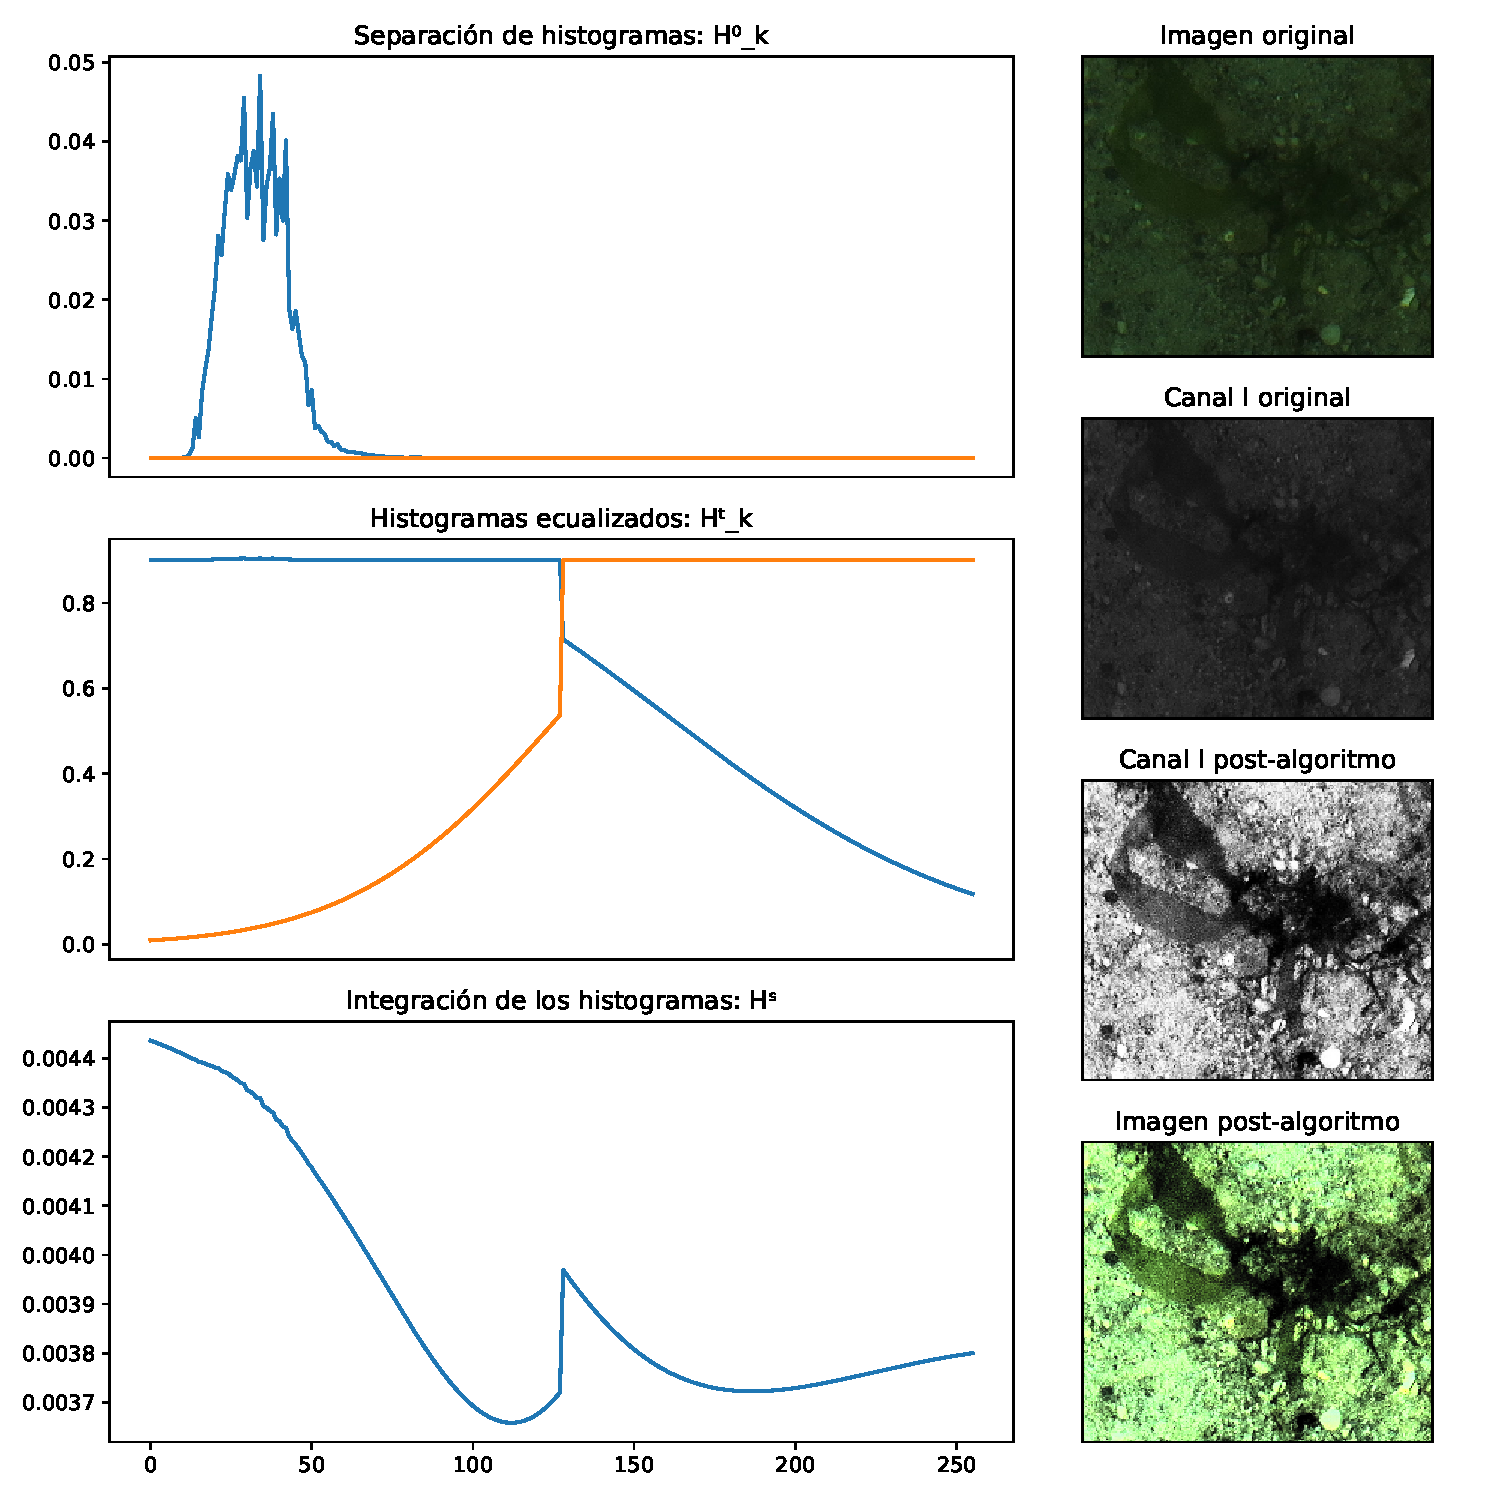
\includegraphics[height=9cm]{imgs/1906bxx-11.pdf}
  \caption{\texttt{[1, 1]}}
\end{minipage}
\hfill
\begin{minipage}[c]{0.48\linewidth}
  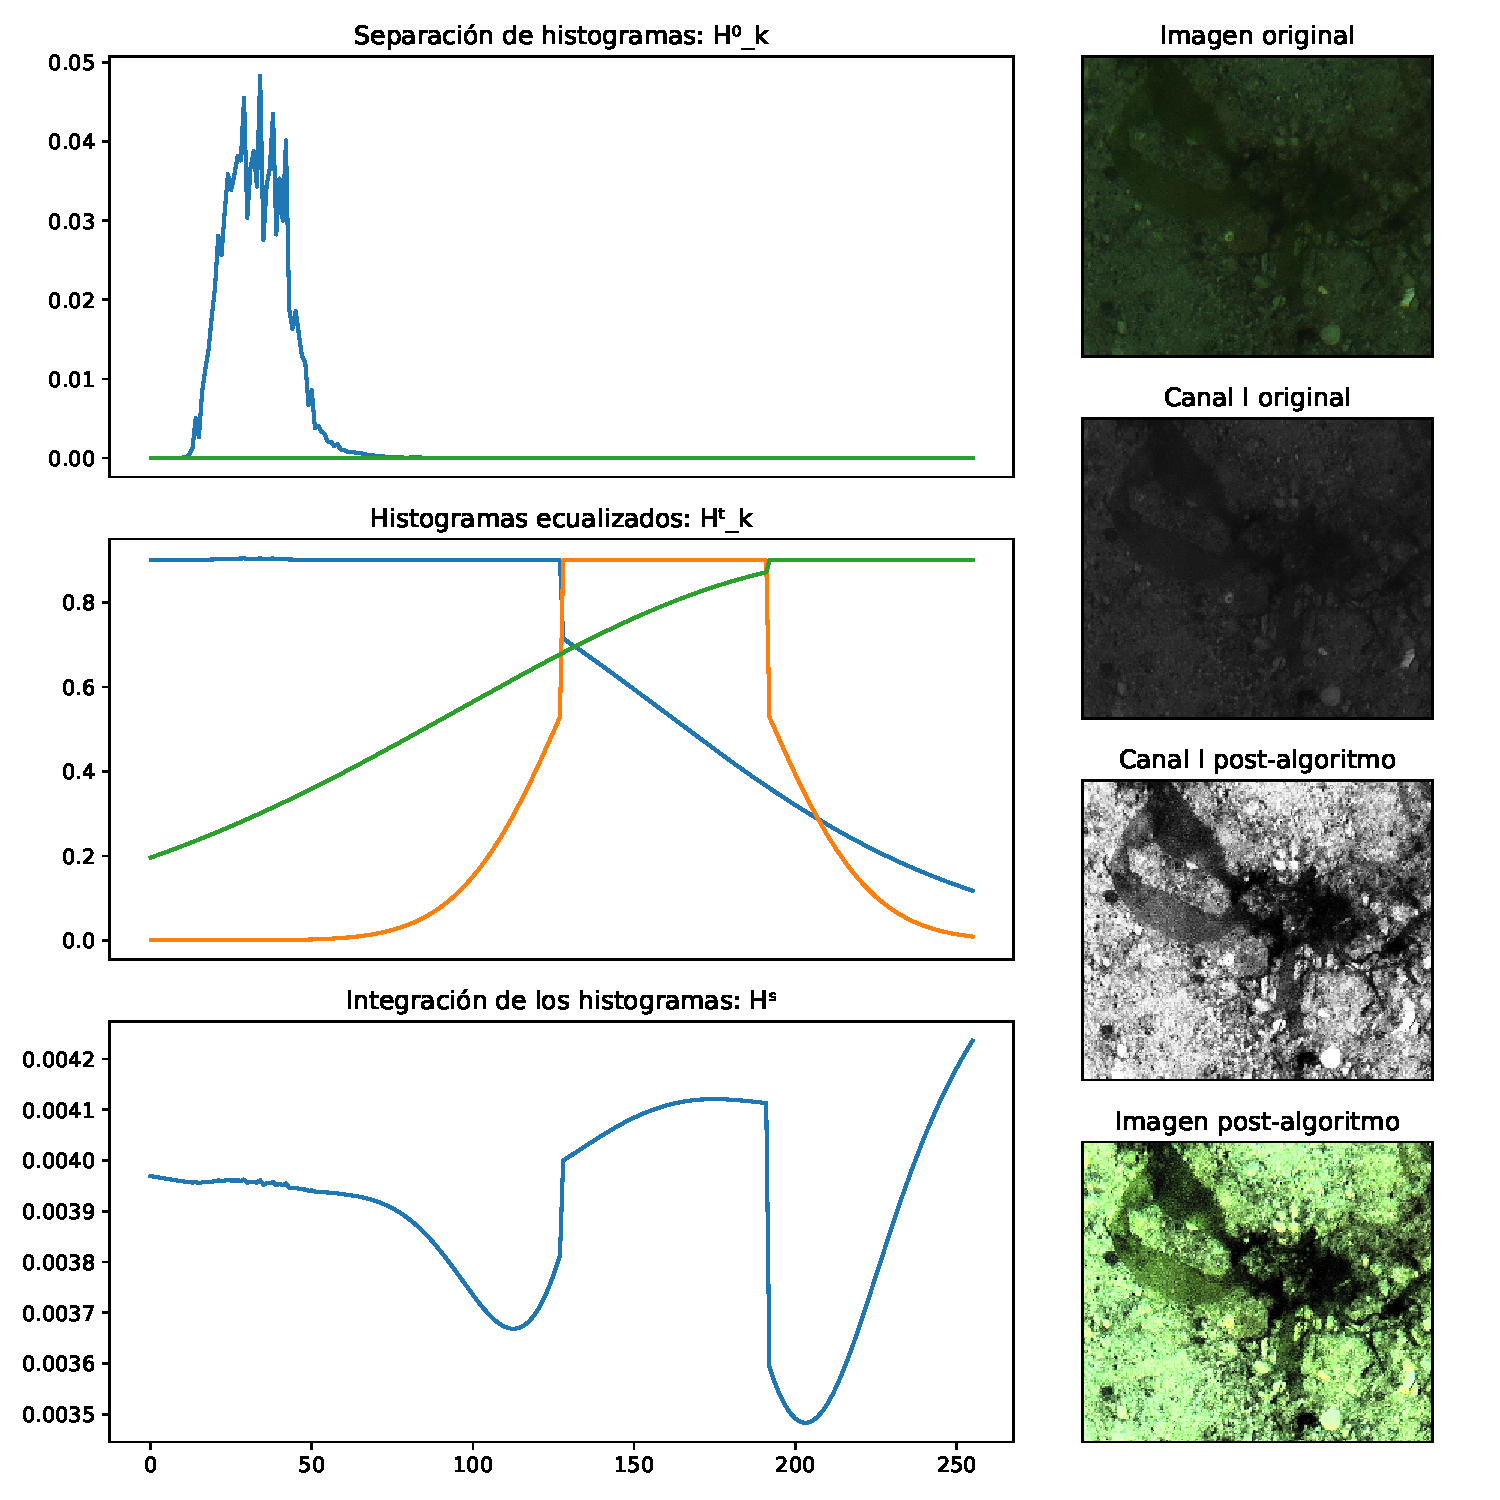
\includegraphics[height=9cm]{imgs/1906bxx-211.pdf}
  \caption{\texttt{[2, 1, 1]}}
\end{minipage}%
\end{figure}

i\begin{figure}[H]
\begin{minipage}[c]{0.48\linewidth}
  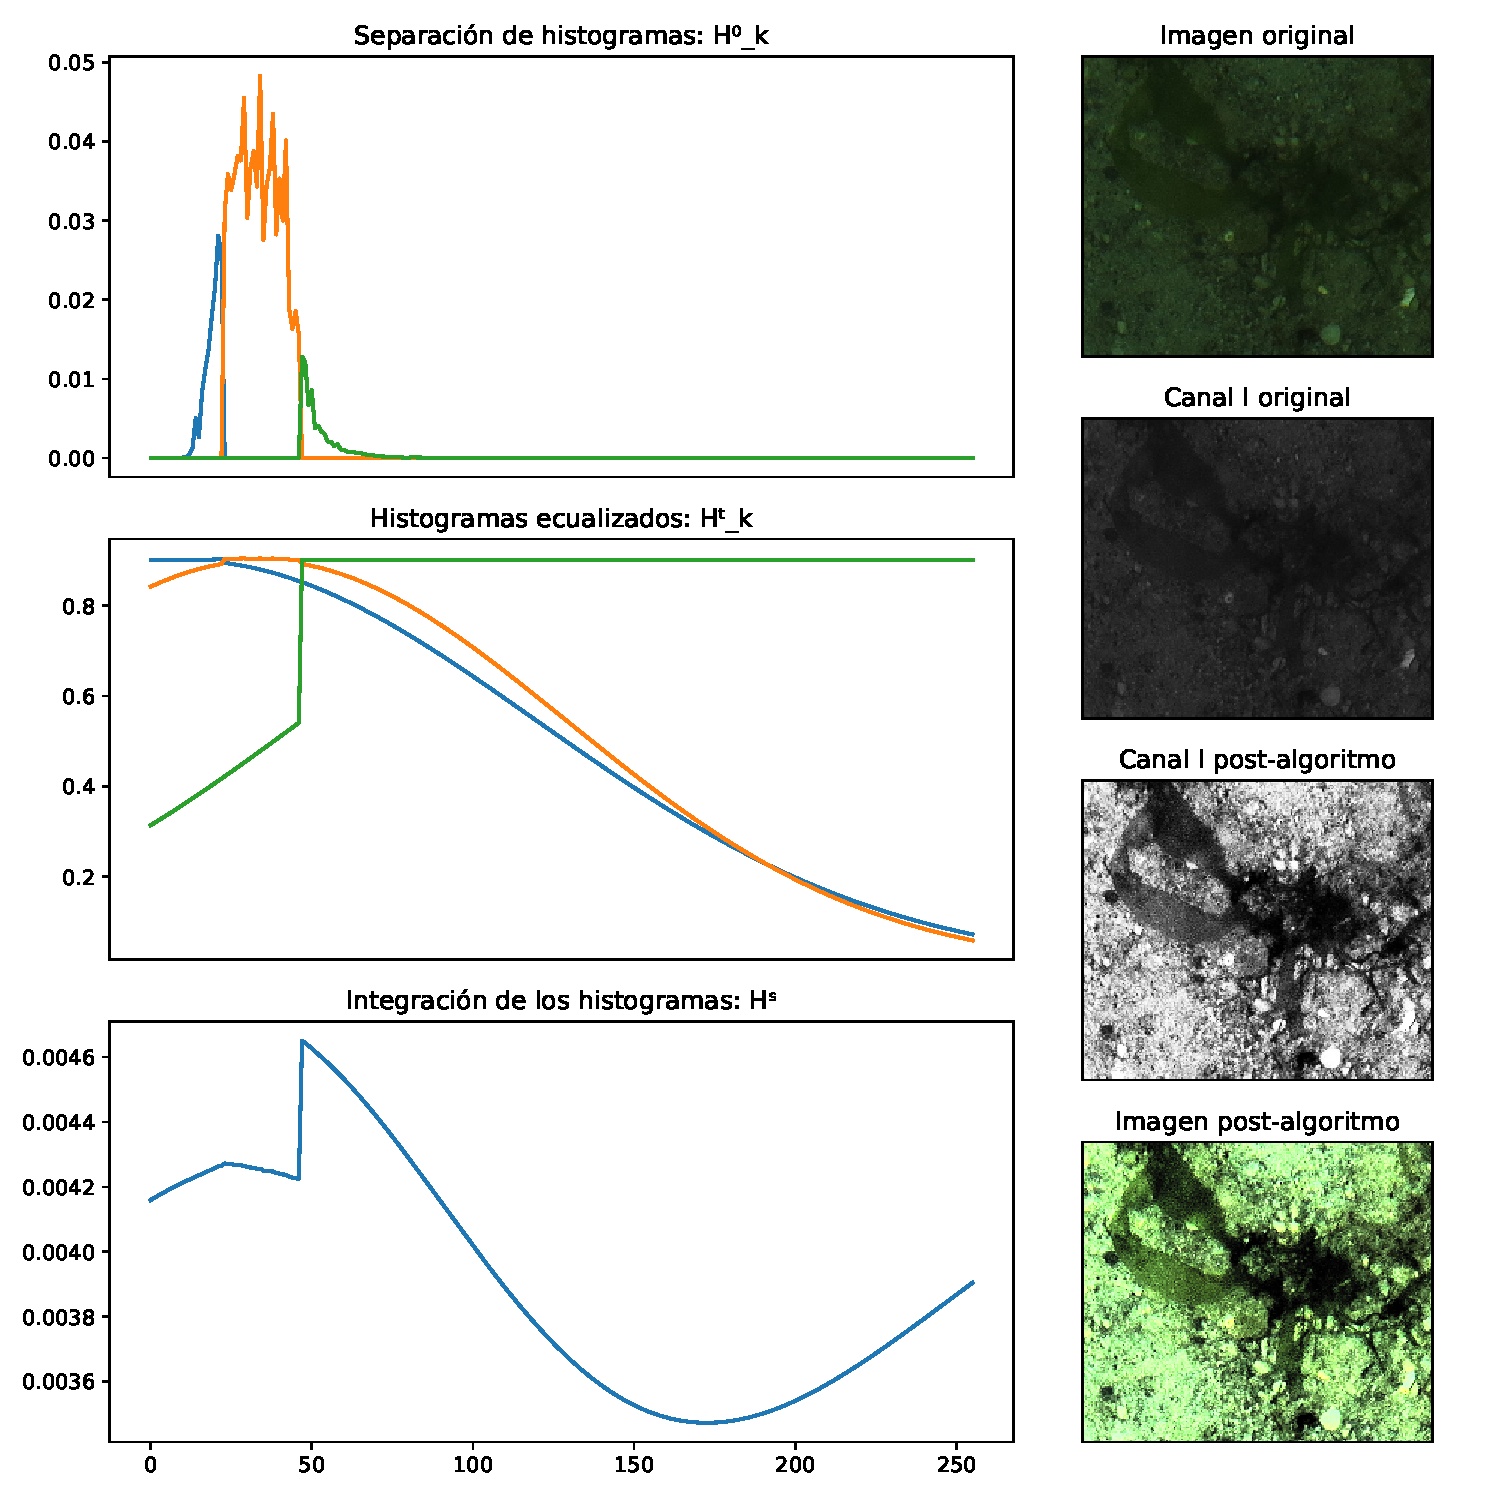
\includegraphics[height=9cm]{imgs/1906bxx-119.pdf}
  \caption{\texttt{[1, 1, 9]}}
\end{minipage}
\hfill
\begin{minipage}[c]{0.48\linewidth}
  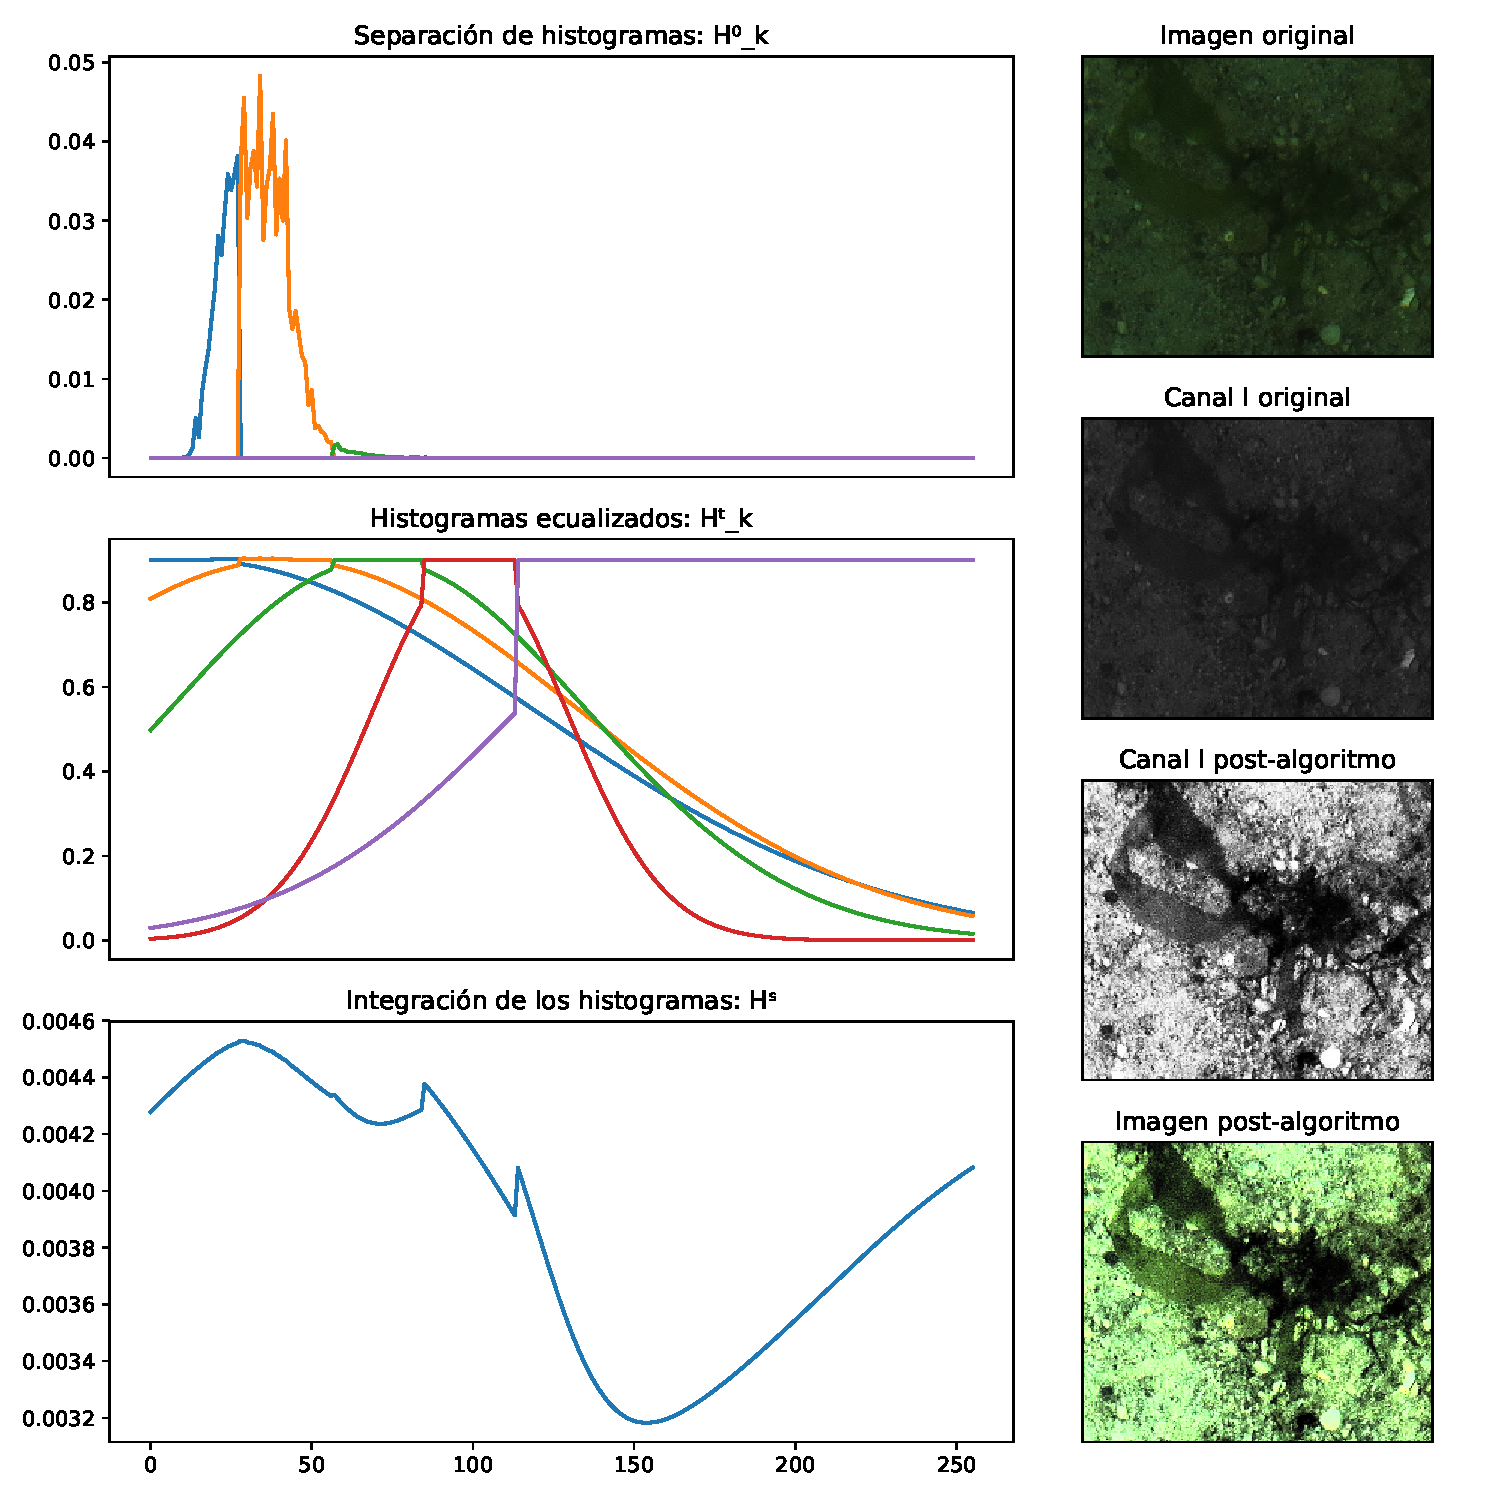
\includegraphics[height=9cm]{imgs/1906bxx-11115.pdf}
  \caption{\texttt{[1, 1, 1, 1, 5]}}
\end{minipage}%
\end{figure}

\subsection{Ejemplo 2}
Usamos la imagen \texttt{1906bxx}, con parámetros $\alpha = 0.8$, $\beta = 0.1$, $\gamma = 0.1$.

\begin{figure}[H]
\begin{minipage}[c]{0.48\linewidth}
  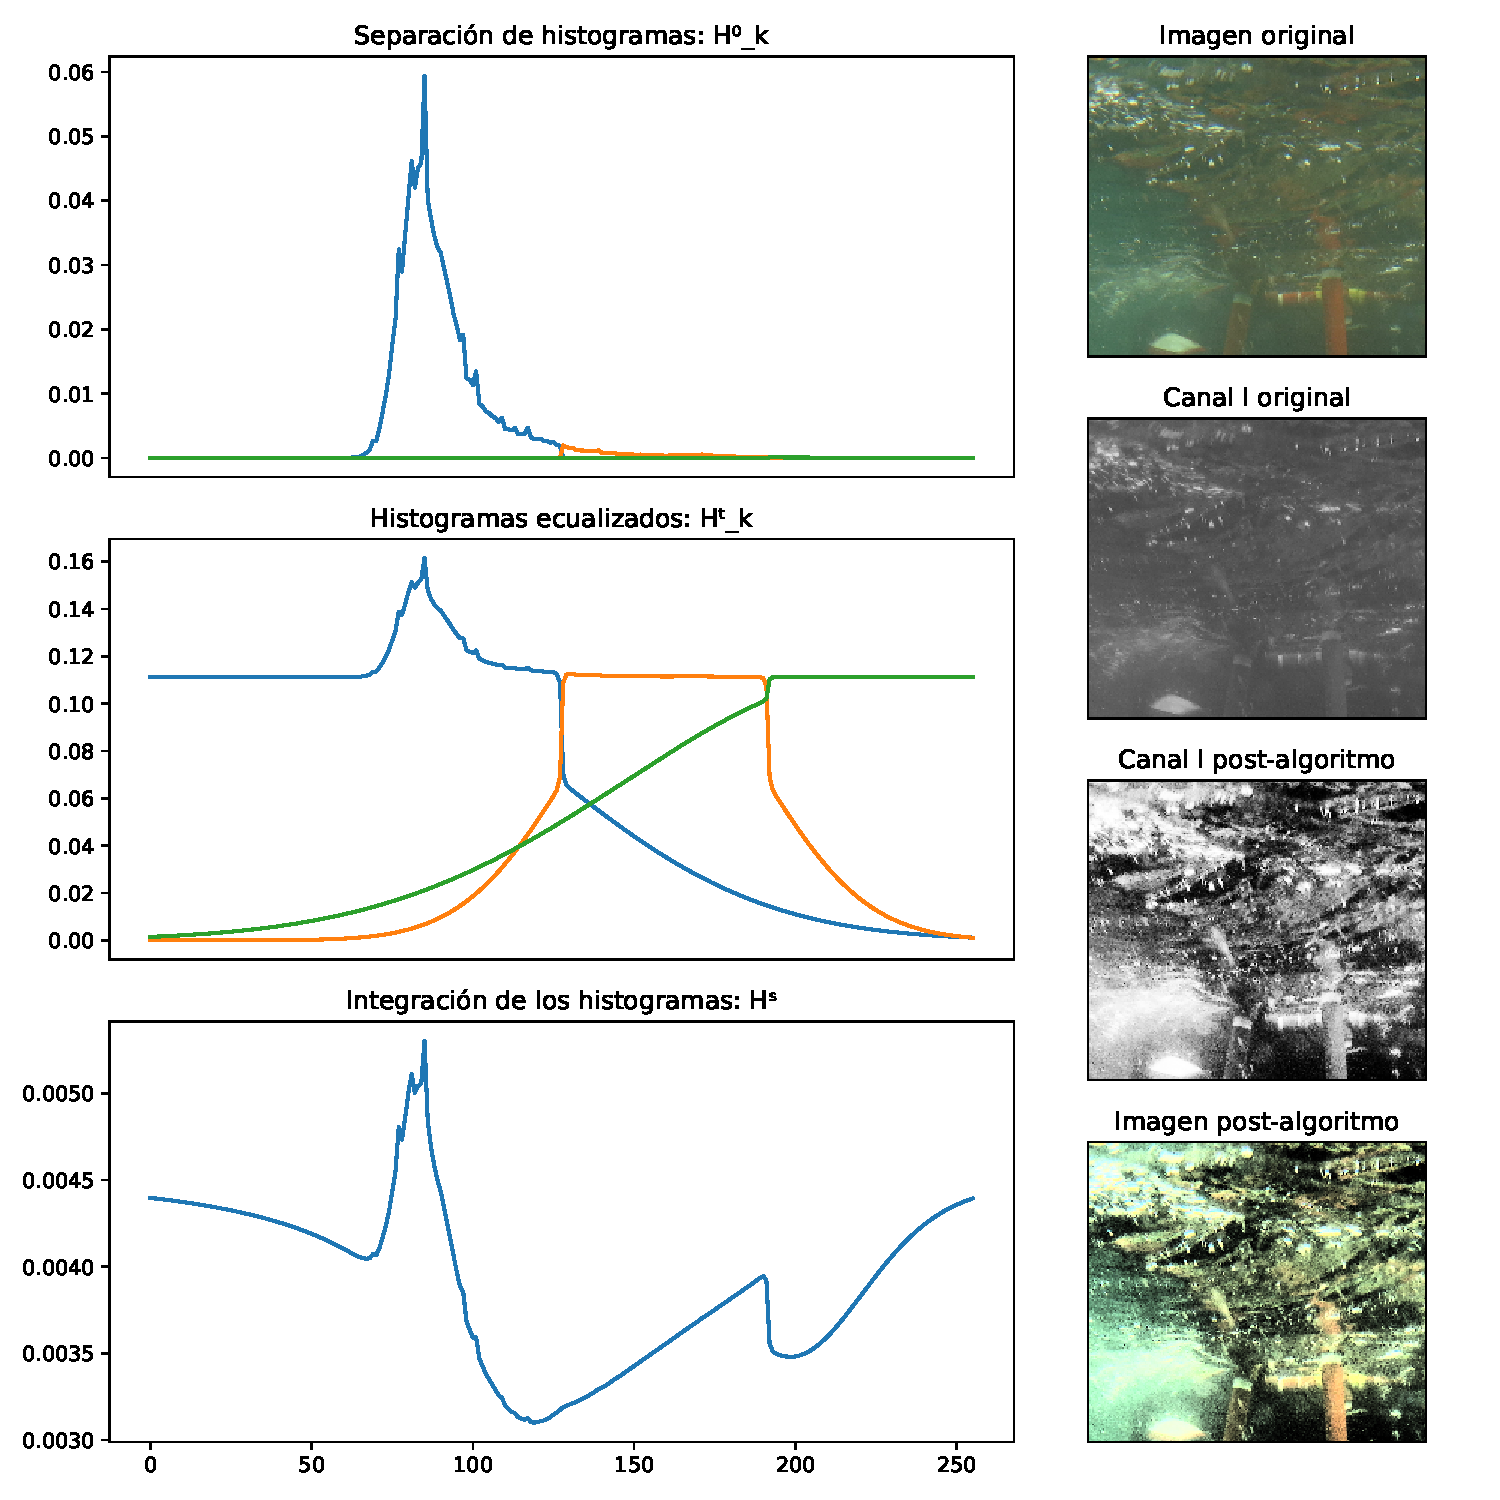
\includegraphics[height=9cm]{imgs/1908iv-211.pdf}
  \caption{\texttt{[2, 1, 1]}}
\end{minipage}
\hfill
\begin{minipage}[c]{0.48\linewidth}
  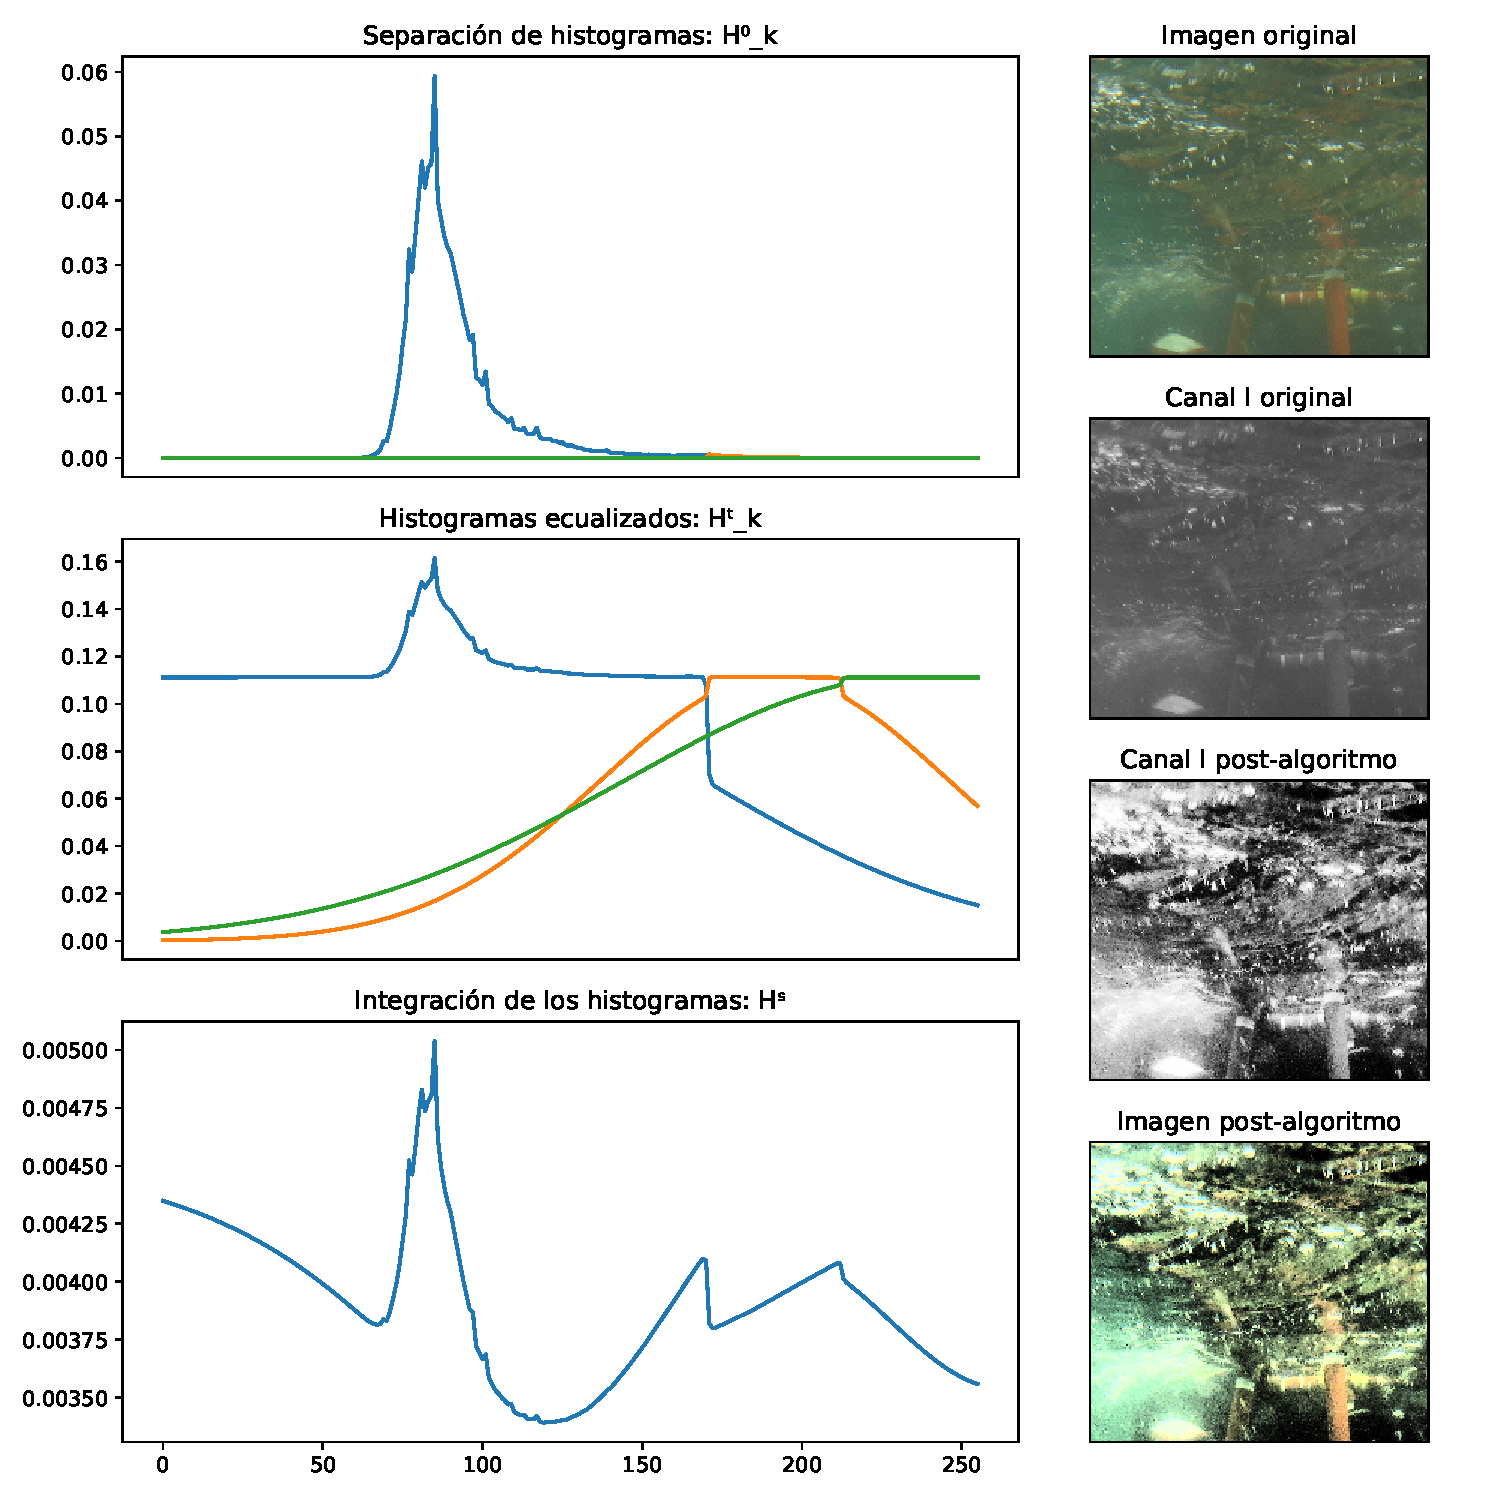
\includegraphics[height=9cm]{imgs/1908iv-411.pdf}
  \caption{\texttt{[4, 1, 1]}}
\end{minipage}%
\end{figure}

i\begin{figure}[H]
\begin{minipage}[c]{0.48\linewidth}
  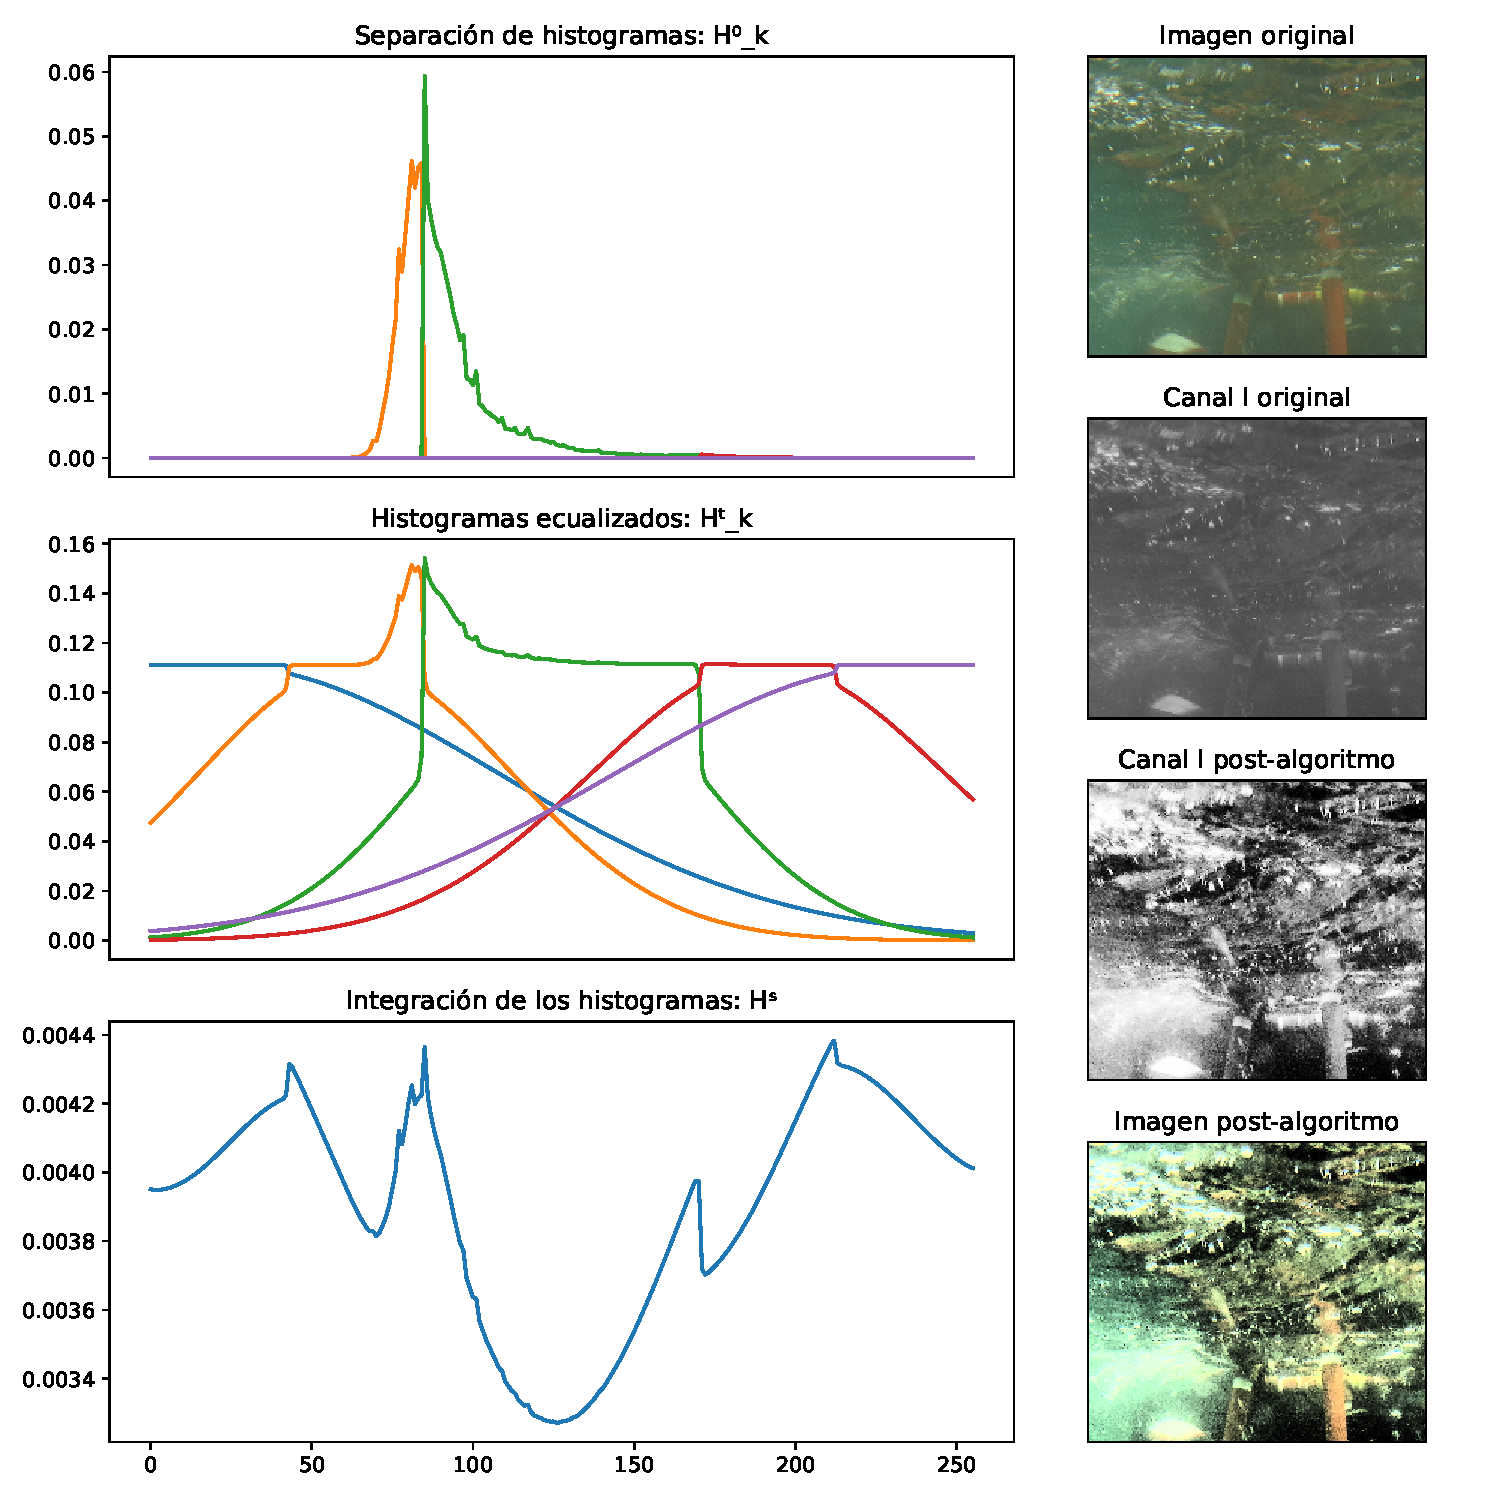
\includegraphics[height=9cm]{imgs/1908iv-11211.pdf}
  \caption{\texttt{[1, 1, 2, 1, 1]}}
\end{minipage}
\hfill
\begin{minipage}[c]{0.48\linewidth}
  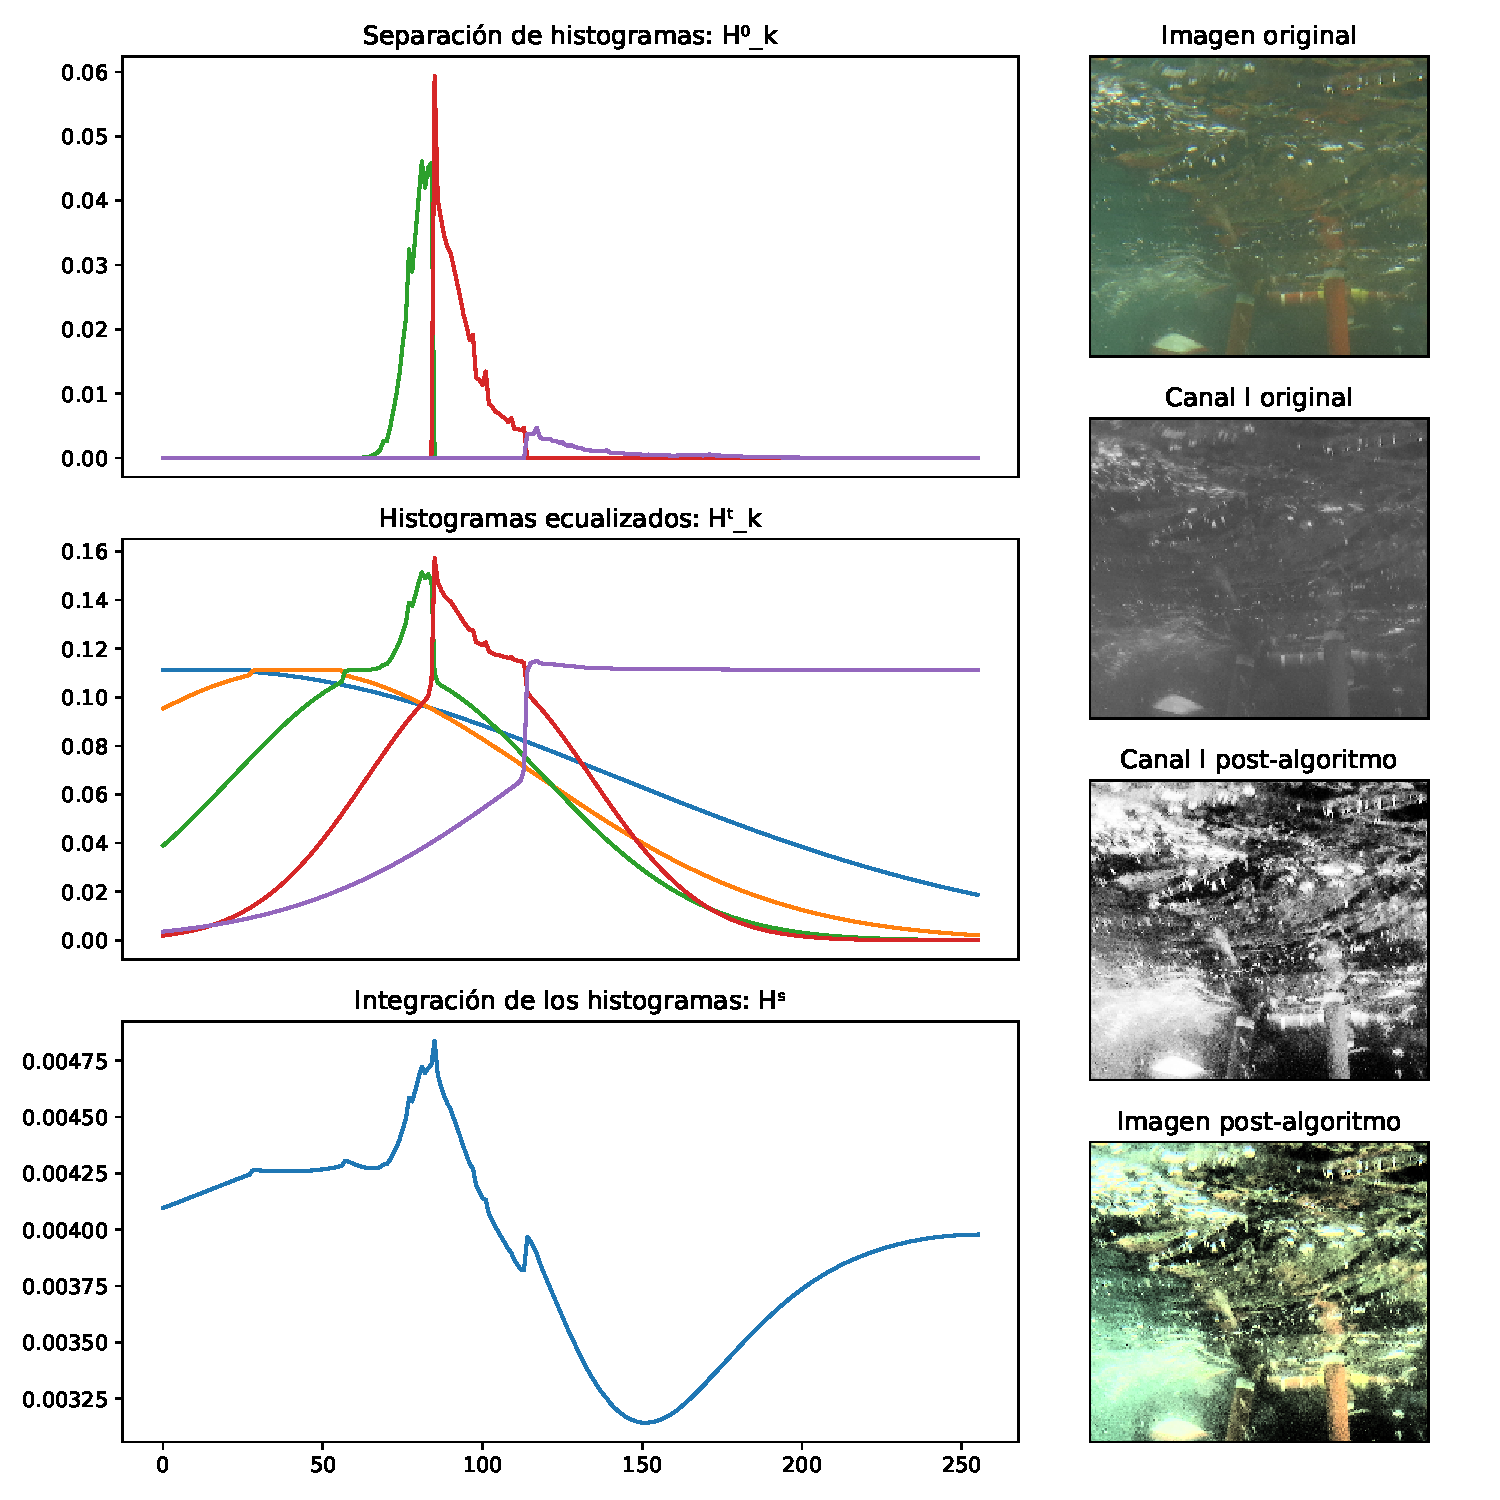
\includegraphics[height=9cm]{imgs/1908iv-11115.pdf}
  \caption{\texttt{[1, 1, 1, 1, 5]}}
\end{minipage}%
\end{figure}

\subsection{Ejemplo 3}
Usamos la imagen \texttt{backlight-la-nacion}, con parámetros $\alpha = 0.5$, $\beta = 0.4$, $\gamma = 0.1$.

\begin{figure}[H]
\begin{minipage}[c]{0.48\linewidth}
  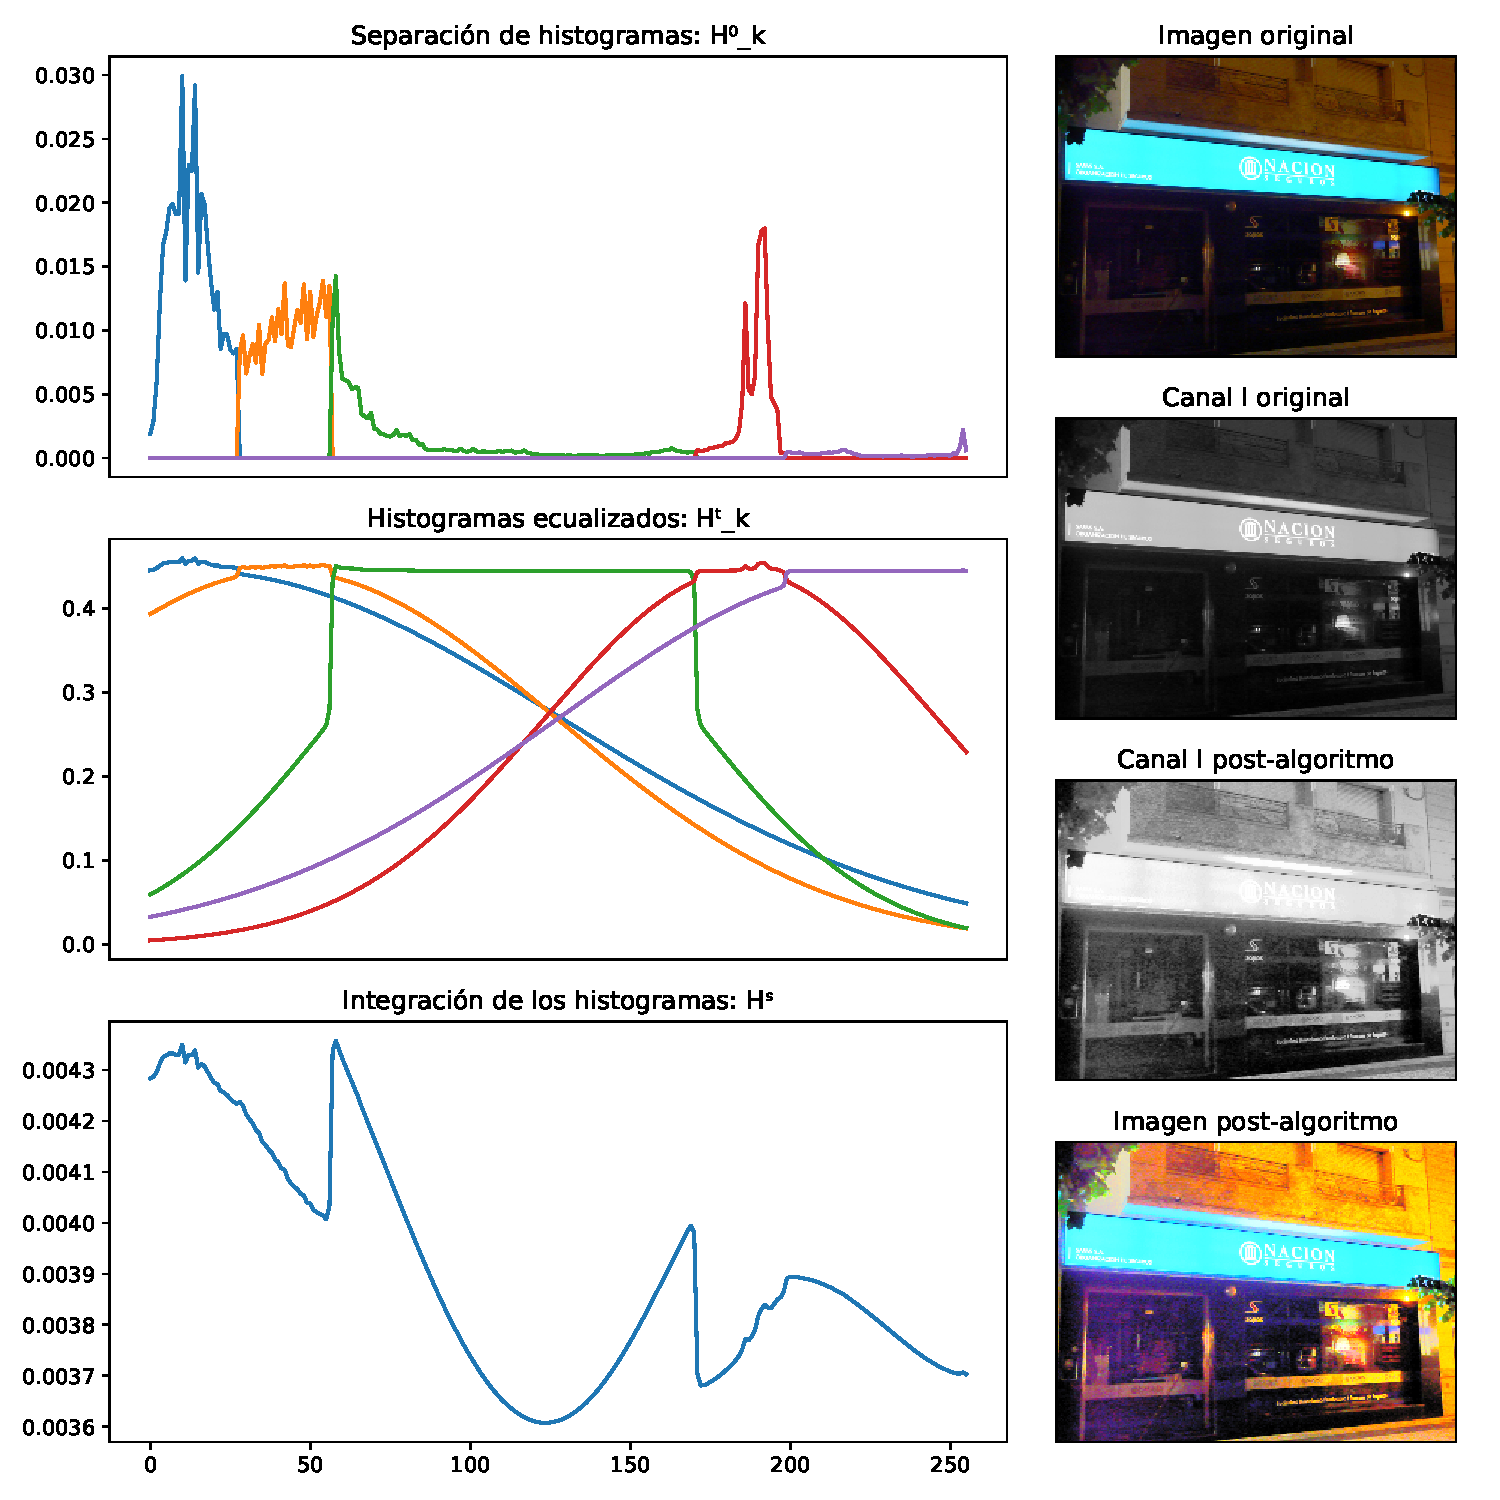
\includegraphics[height=9cm]{imgs/backlightnacion-11412.pdf}
  \caption{\texttt{[1, 1, 4, 1, 2]}}
\end{minipage}
\hfill
\begin{minipage}[c]{0.48\linewidth}
  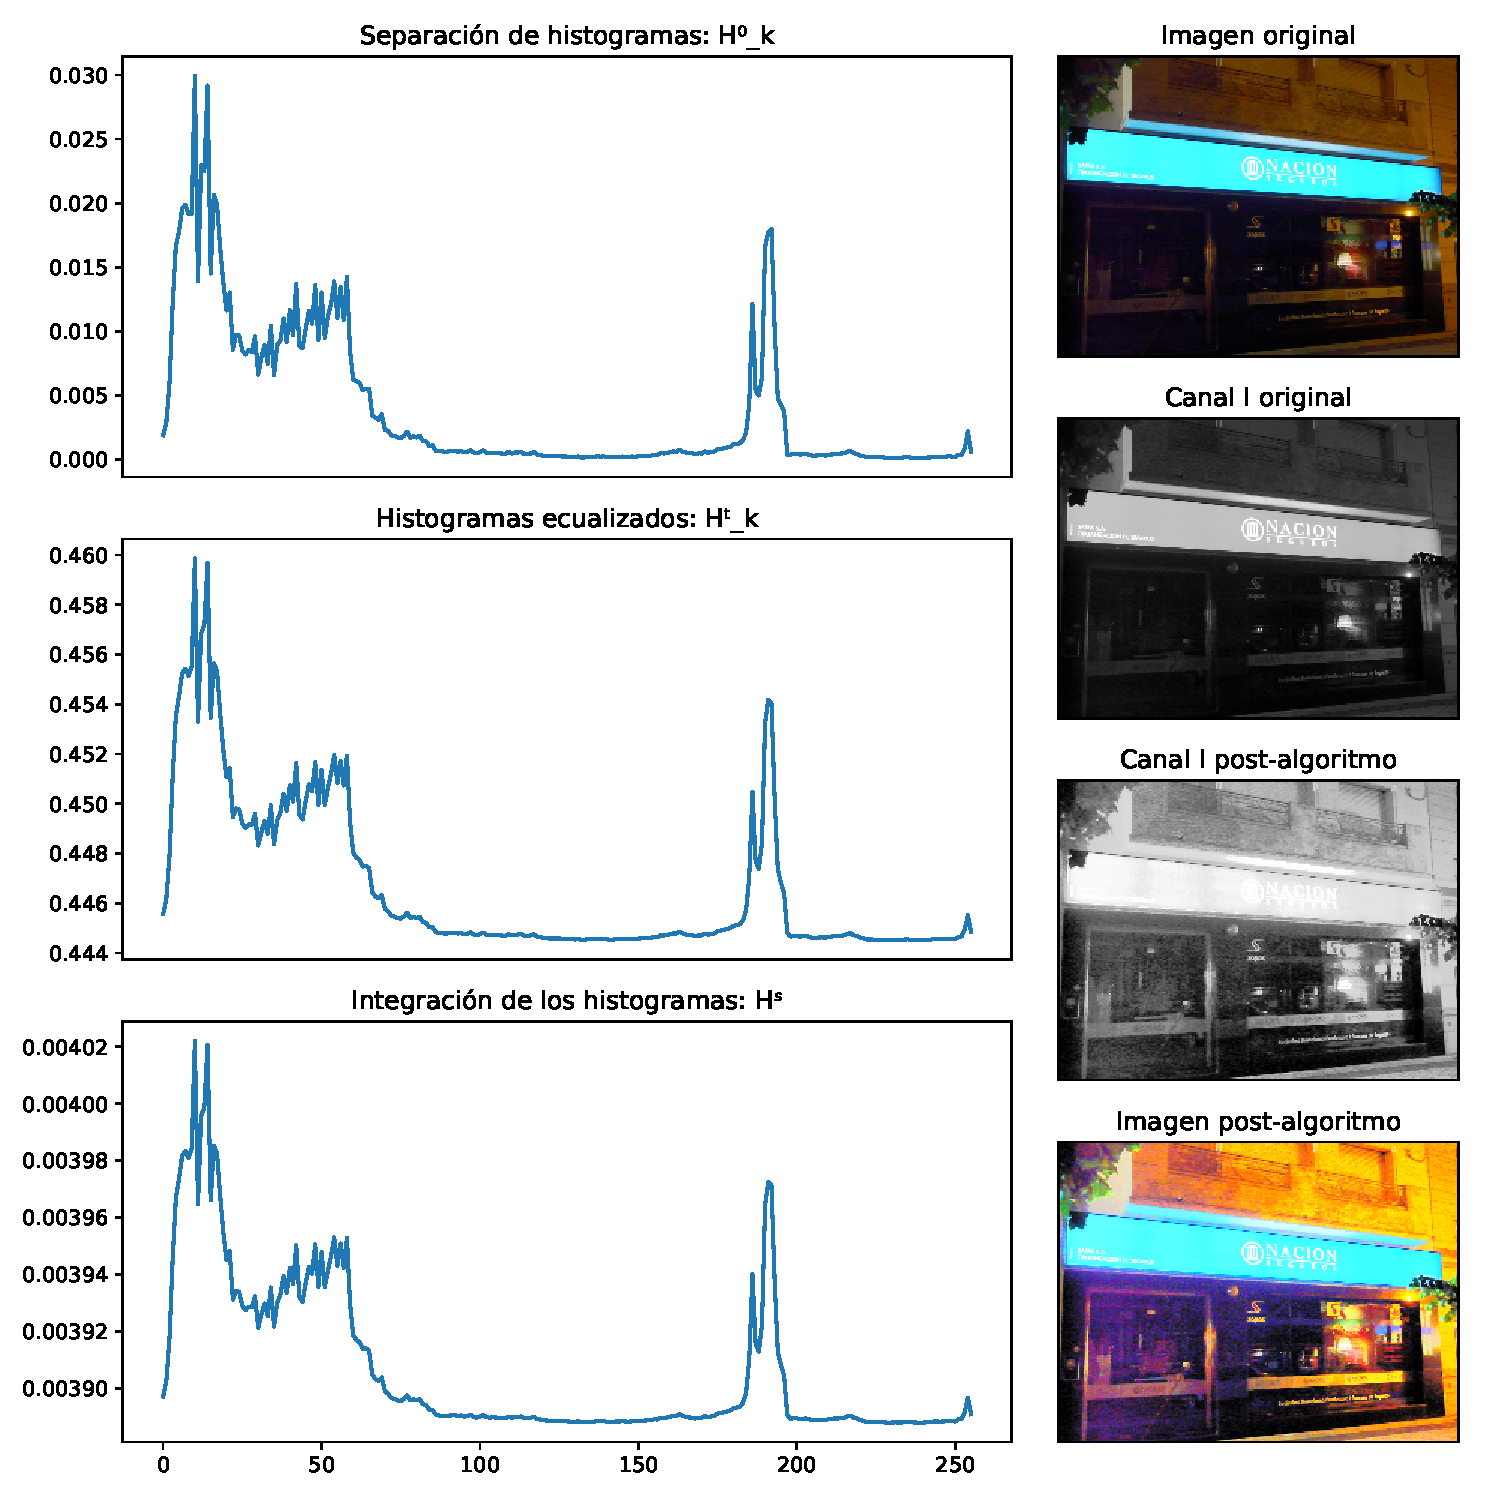
\includegraphics[height=9cm]{imgs/backlightnacion-1.pdf}
  \caption{\texttt{[1]}}
\end{minipage}%
\end{figure}

\begin{figure}[H]
\begin{minipage}[c]{0.48\linewidth}
  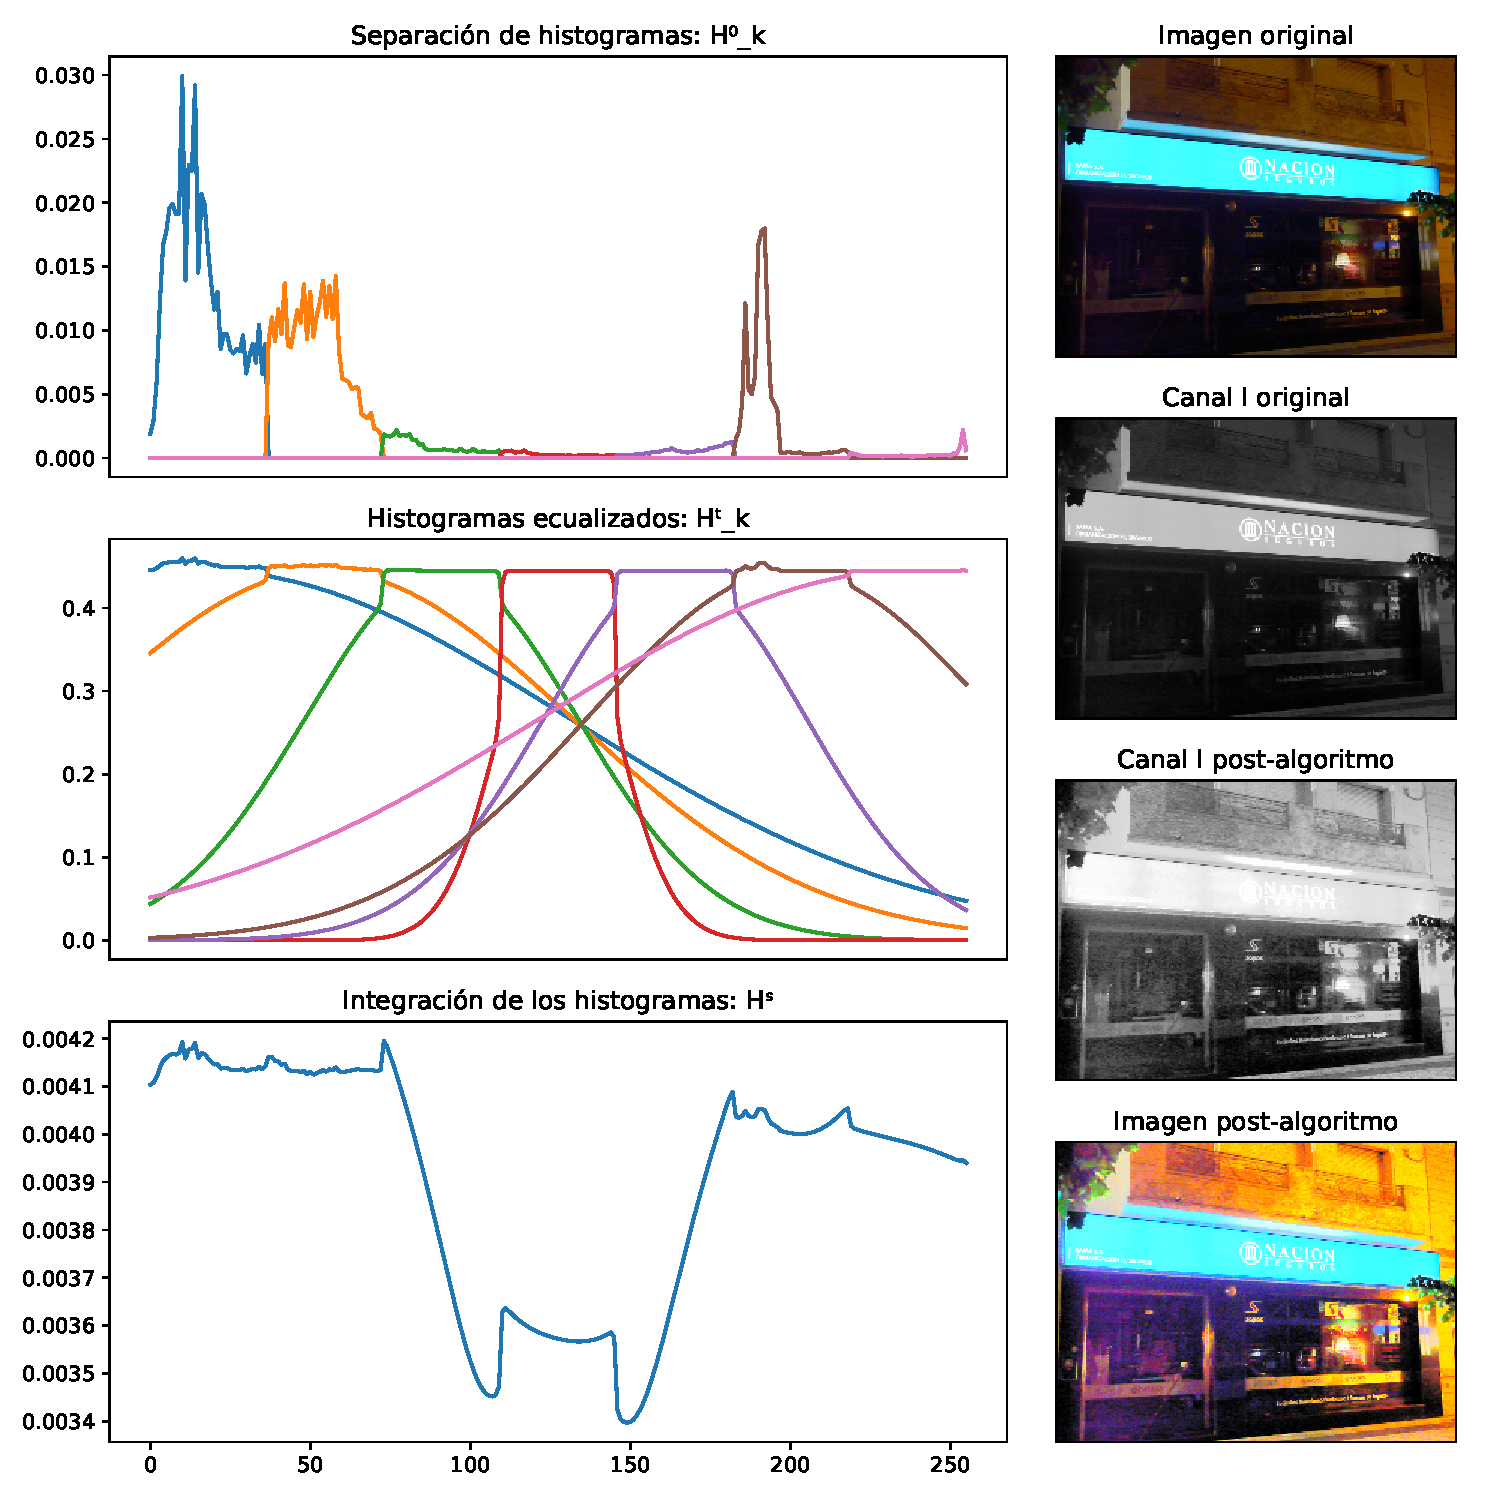
\includegraphics[height=9cm]{imgs/backlightnacion-1111111.pdf}
  \caption{\texttt{[1, 1, 4, 1, 2]}}
\end{minipage}
\hfill
\begin{minipage}[c]{0.48\linewidth}
  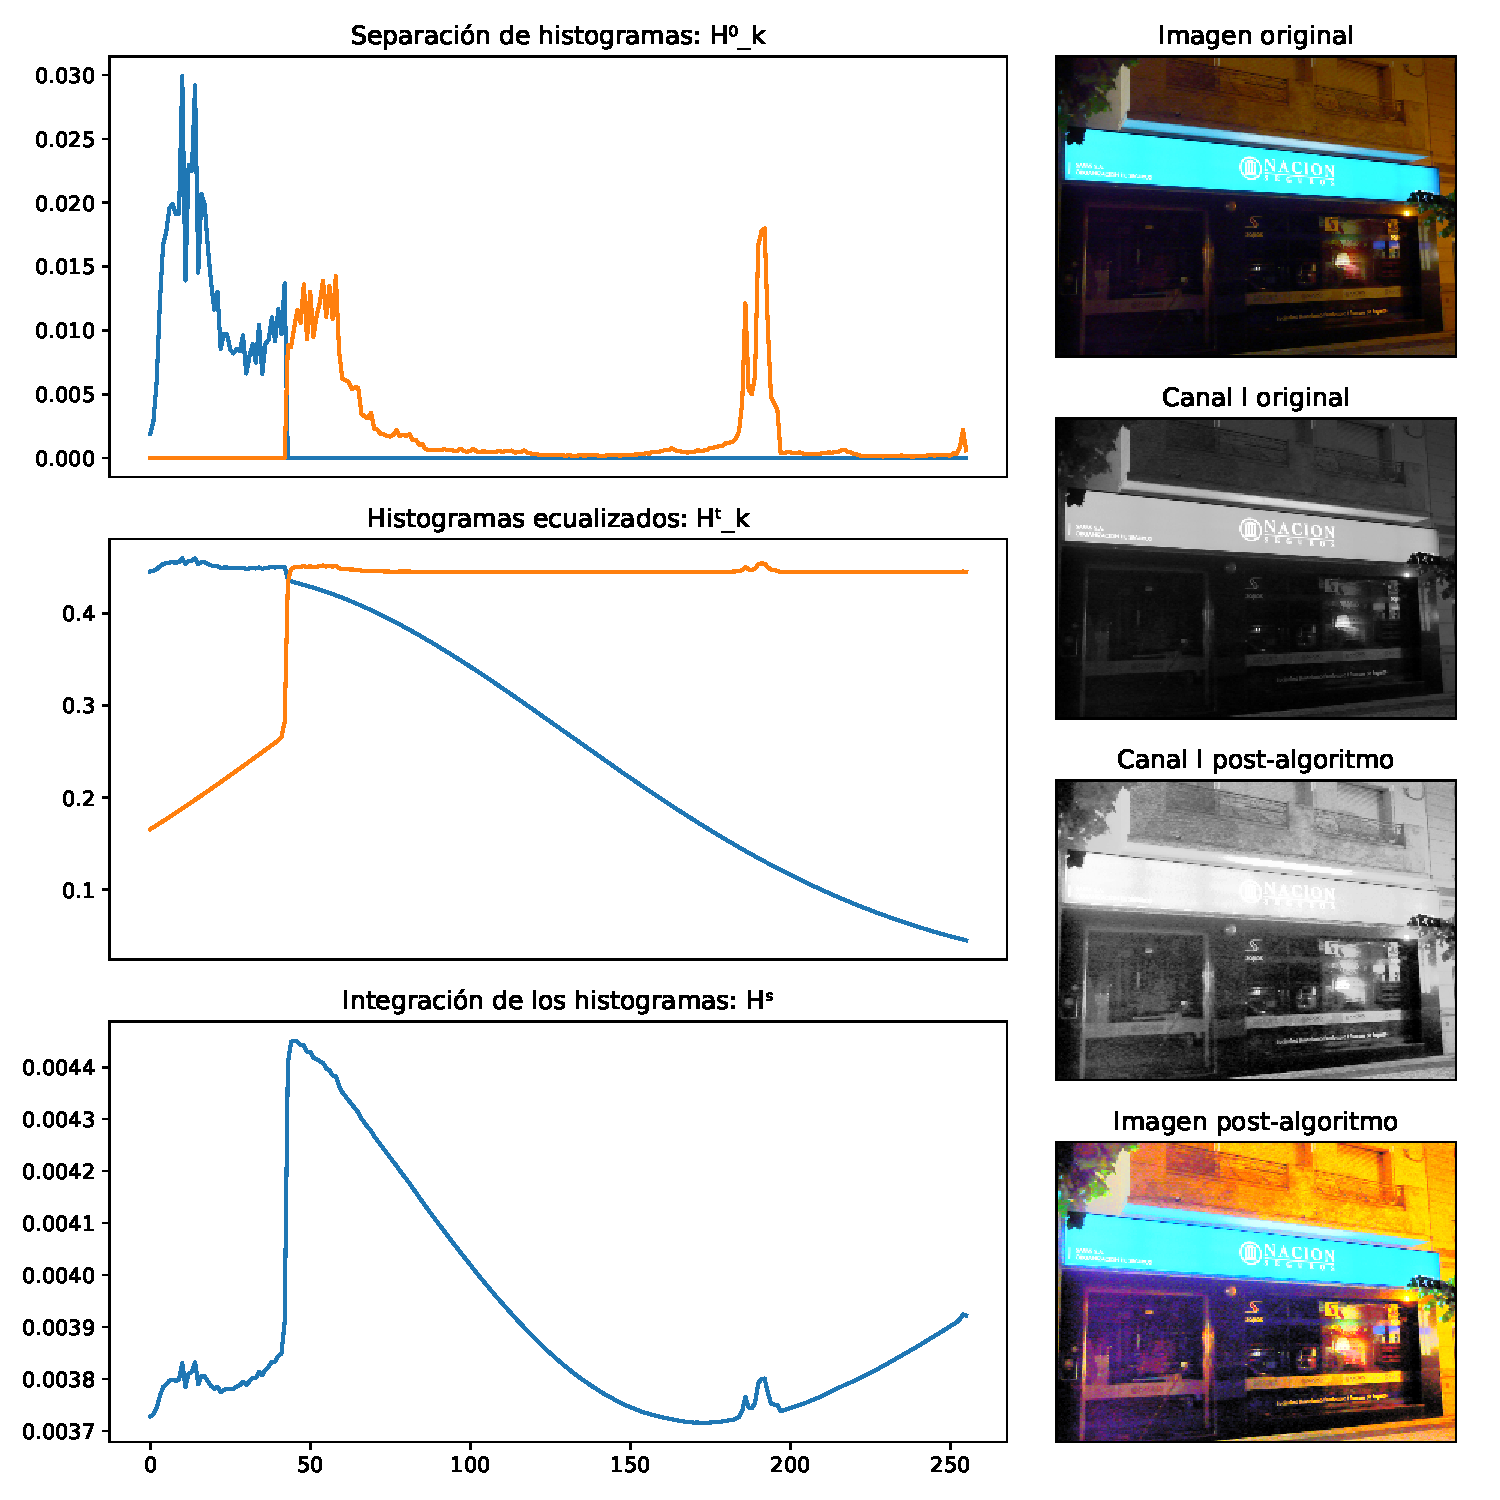
\includegraphics[height=9cm]{imgs/backlightnacion-15.pdf}
  \caption{\texttt{[1]}}
\end{minipage}%
\end{figure}

\newpage

\section{Estudio sobre la variación de los parámetros}
\par En las siguientes figuras se puede ver el algoritmo corrido con distintos valores de $\alpha, \beta$ y $\gamma$.

\par Se observa que mayores valores de $\alpha$ preservan los histogramas originales;
mayores valores de $\beta$ reducen su impacto;
mayores valores de $\gamma$ suavizan el histograma resultante.

\par En particular, con $\alpha = 1$, $H^s = H^0$; con $\beta = 1$, $\forall H^0, H^s = h$\footnote{Con $h$ el $H^t$ resultante de tener un $H^0$ nulo, con $\alpha = 1$.}.

\par Si bien los resultados varían cuantitativamente junto a los parámetros, las únicas diferencias cualitativas se notan para valores altos de $\alpha$ (dentro del intervalo $[0.9, 1]$ en el primer ejemplo).
Variar $\gamma$ afecta la suavidad del histograma pero no parece efectar la suavidad de la imagen\footnote{De hecho el paper sugiere $\gamma = 0$.}.

\begin{figure}[H]
\begin{minipage}[c]{0.48\linewidth}
  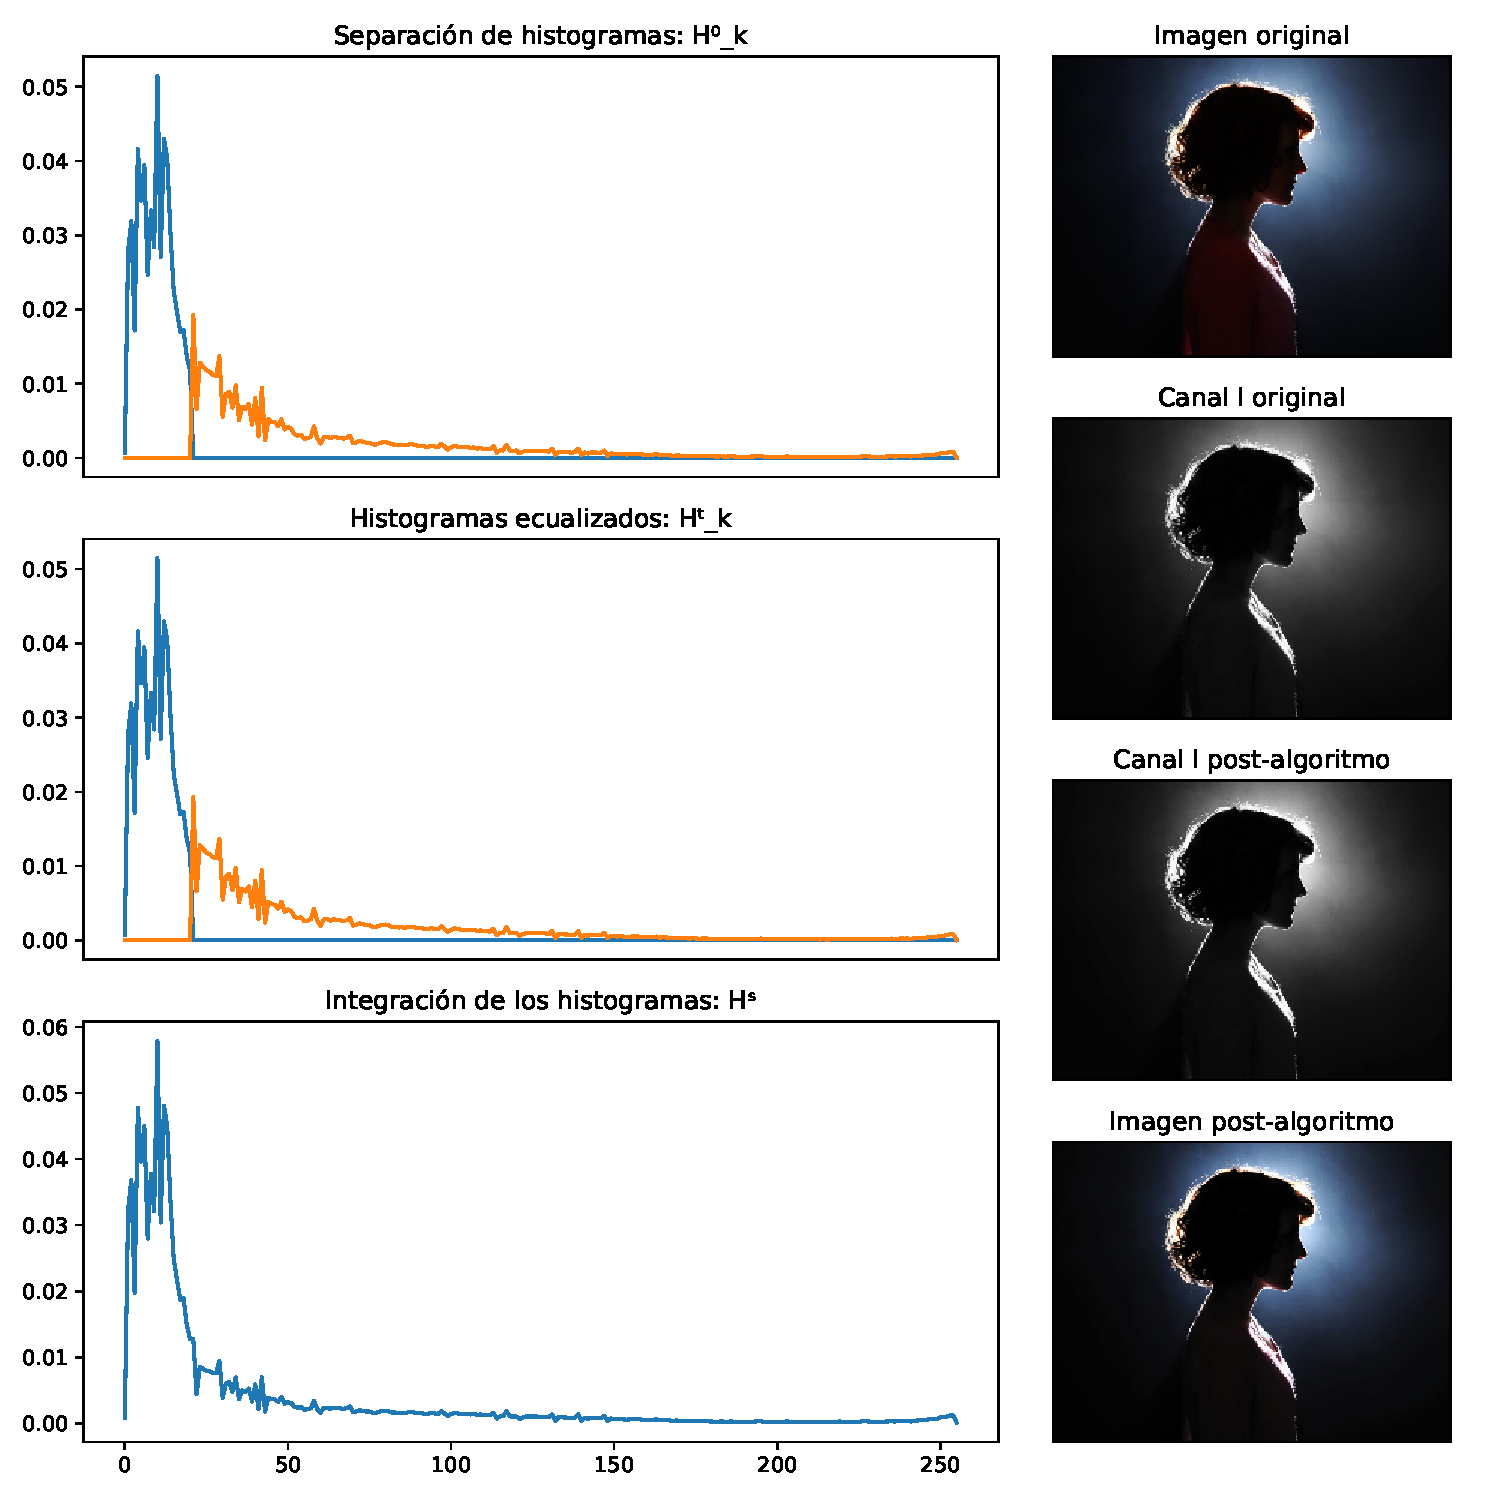
\includegraphics[height=9cm]{imgs/wom-1-0-0.pdf}
  \caption{$\alpha = 1, \beta = 0, \gamma = 0$}
\end{minipage}
\hfill
\begin{minipage}[c]{0.48\linewidth}
  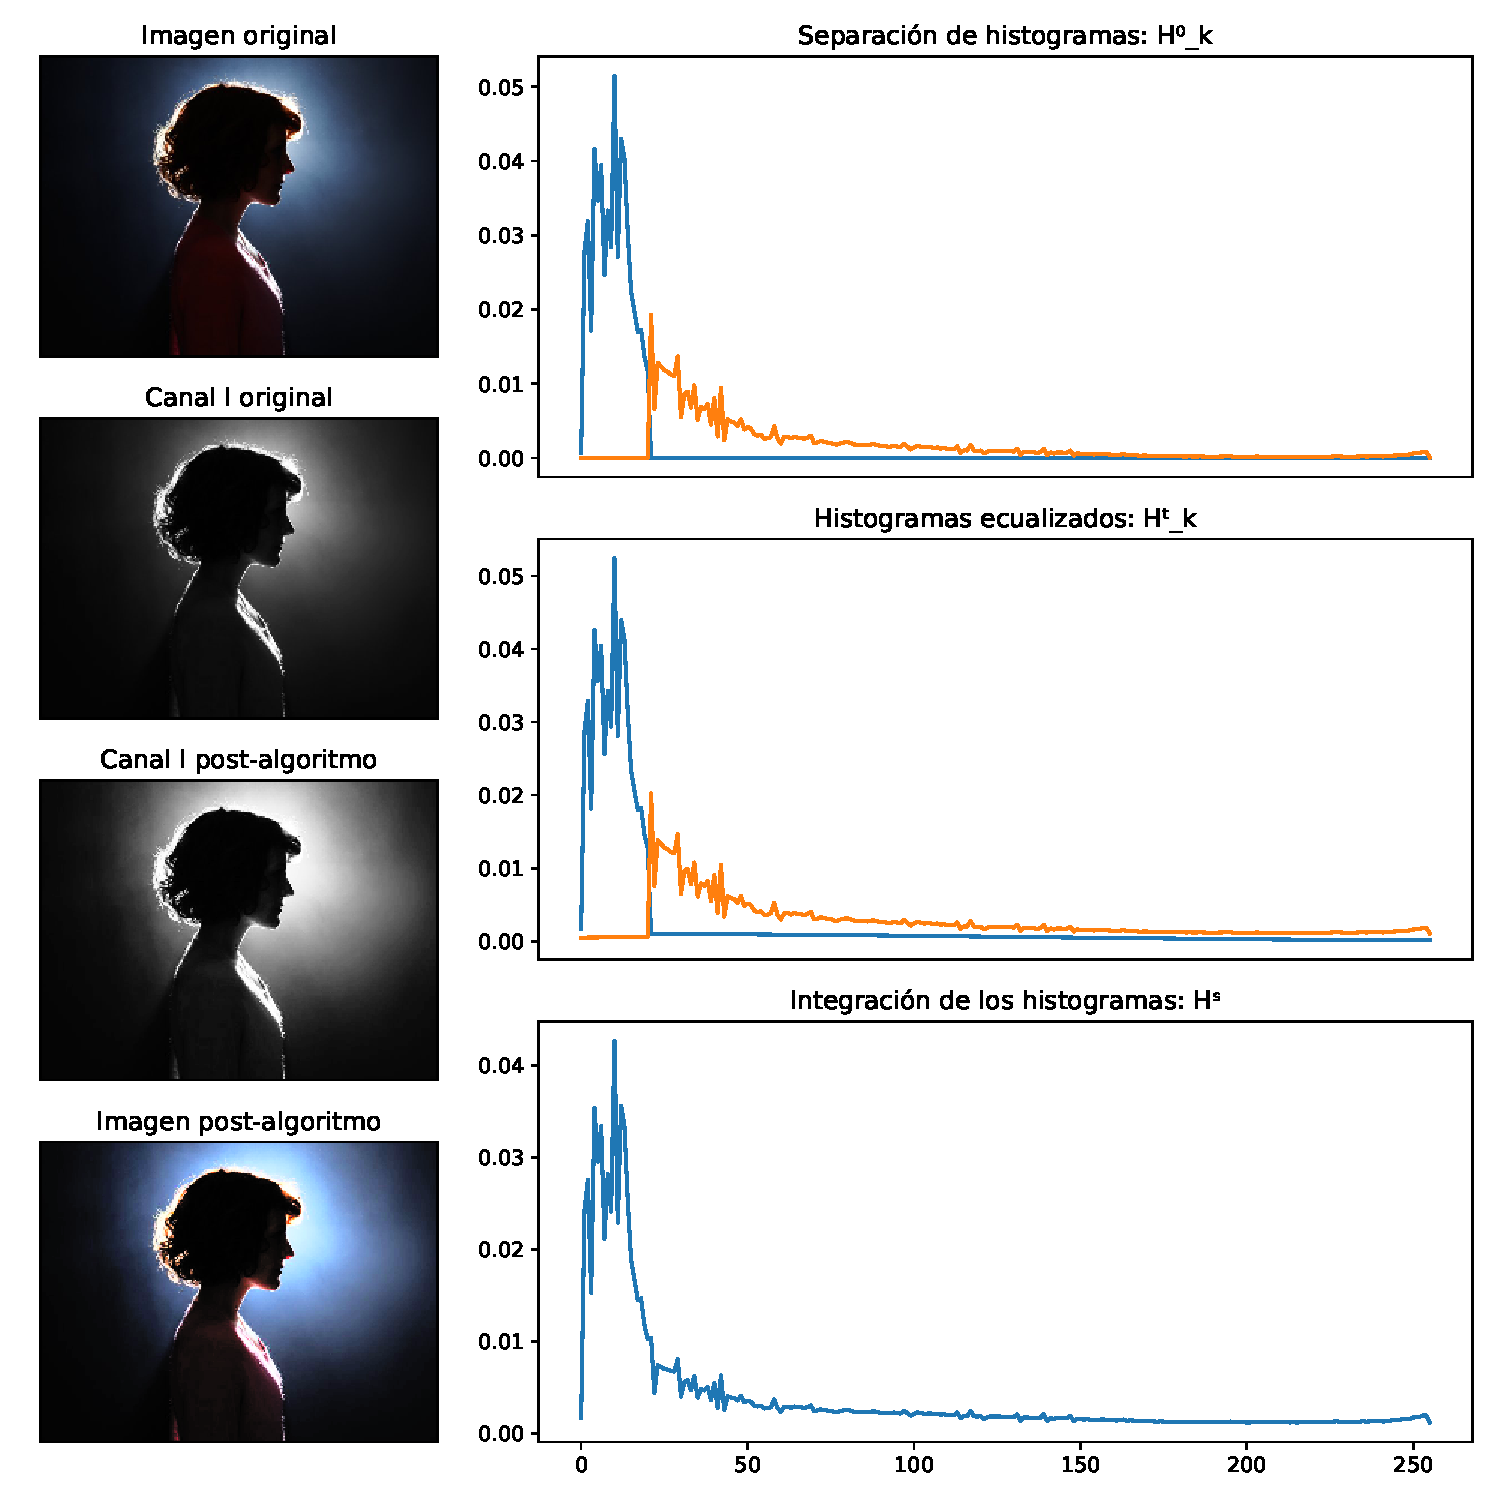
\includegraphics[height=9cm]{imgs/wom-999-001-0.pdf}
  \caption{$\alpha = 0.999, \beta = 0.001, \gamma = 0$}
\end{minipage}%
\end{figure}

\begin{figure}[H]
\begin{minipage}[c]{0.48\linewidth}
  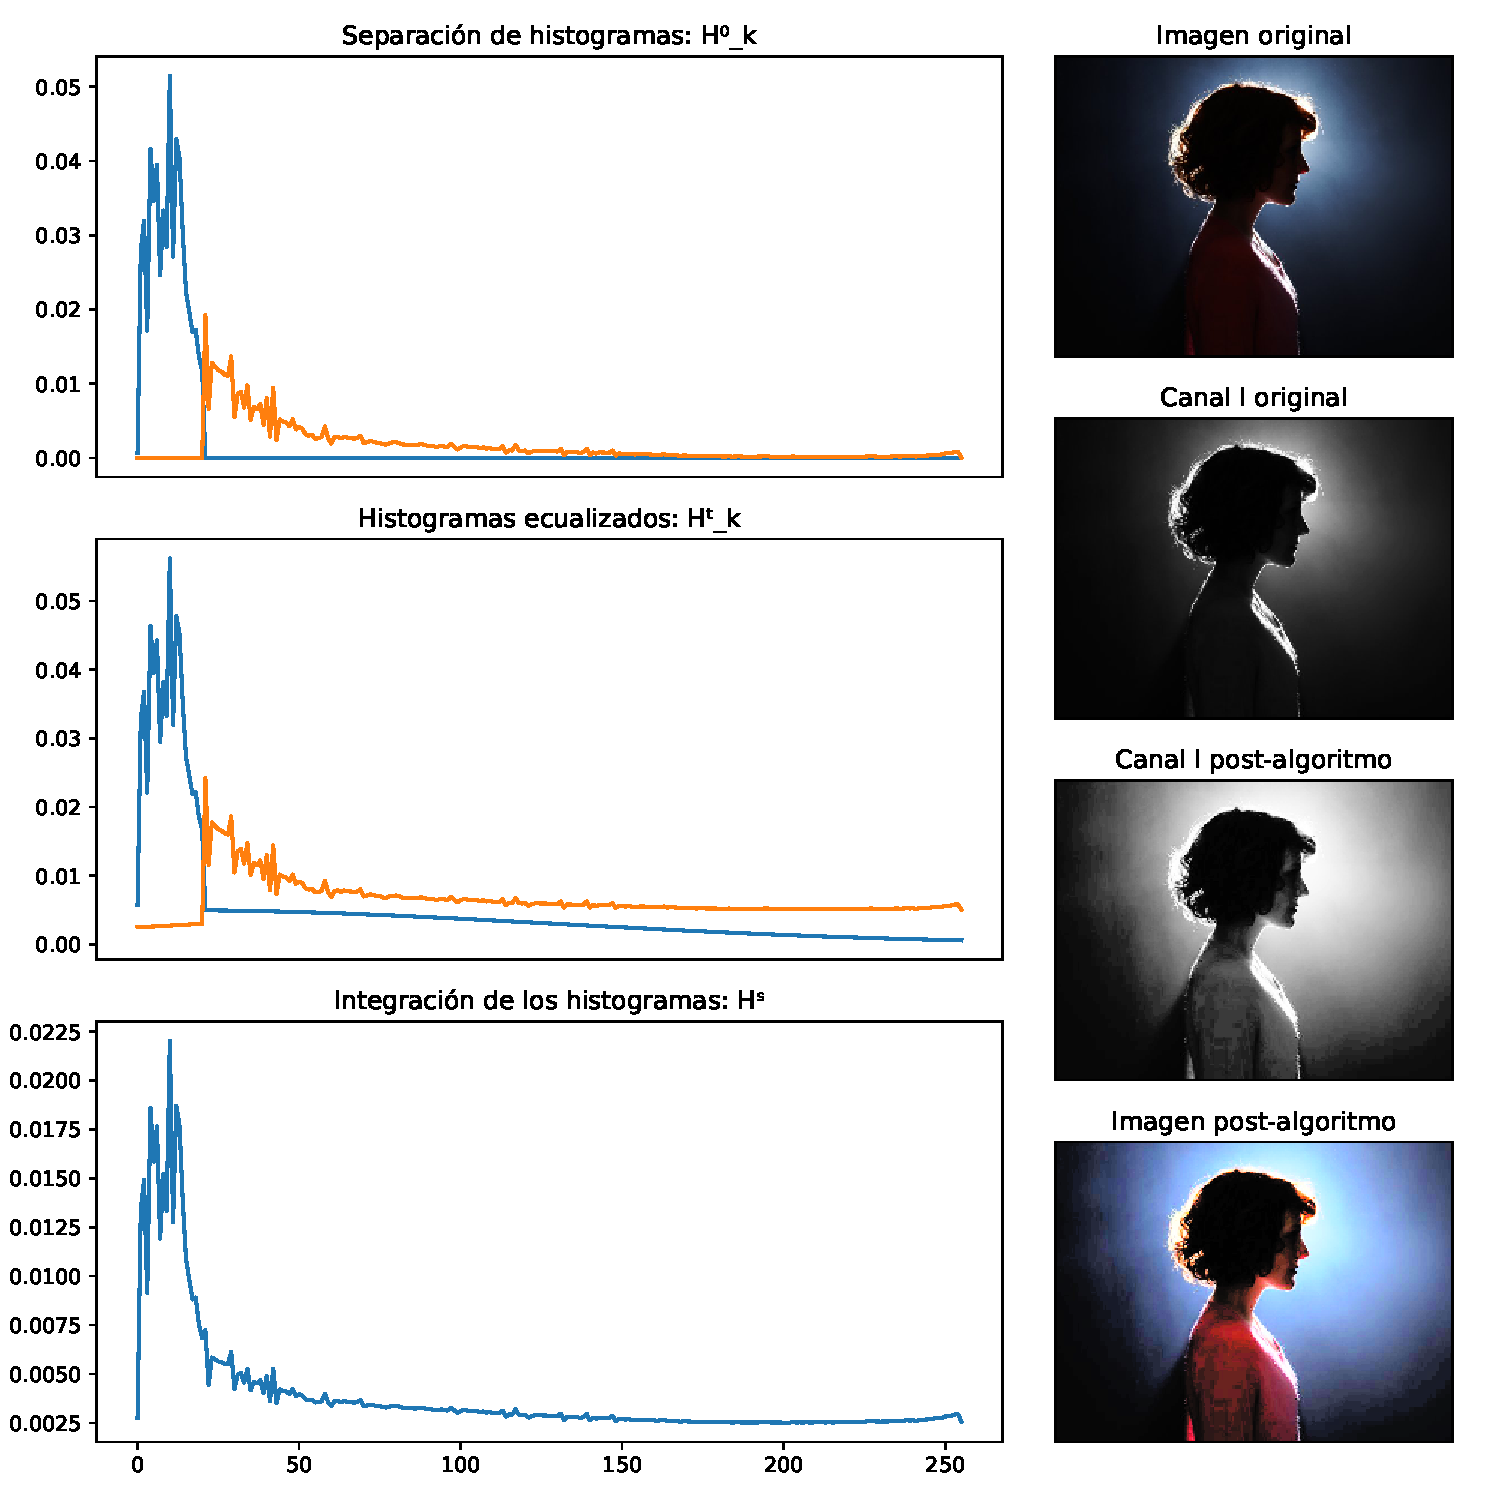
\includegraphics[height=9cm]{imgs/wom-995-005-0.pdf}
  \caption{$\alpha = 0.995, \beta = 0.005, \gamma = 0$}
\end{minipage}
\hfill
\begin{minipage}[c]{0.48\linewidth}
  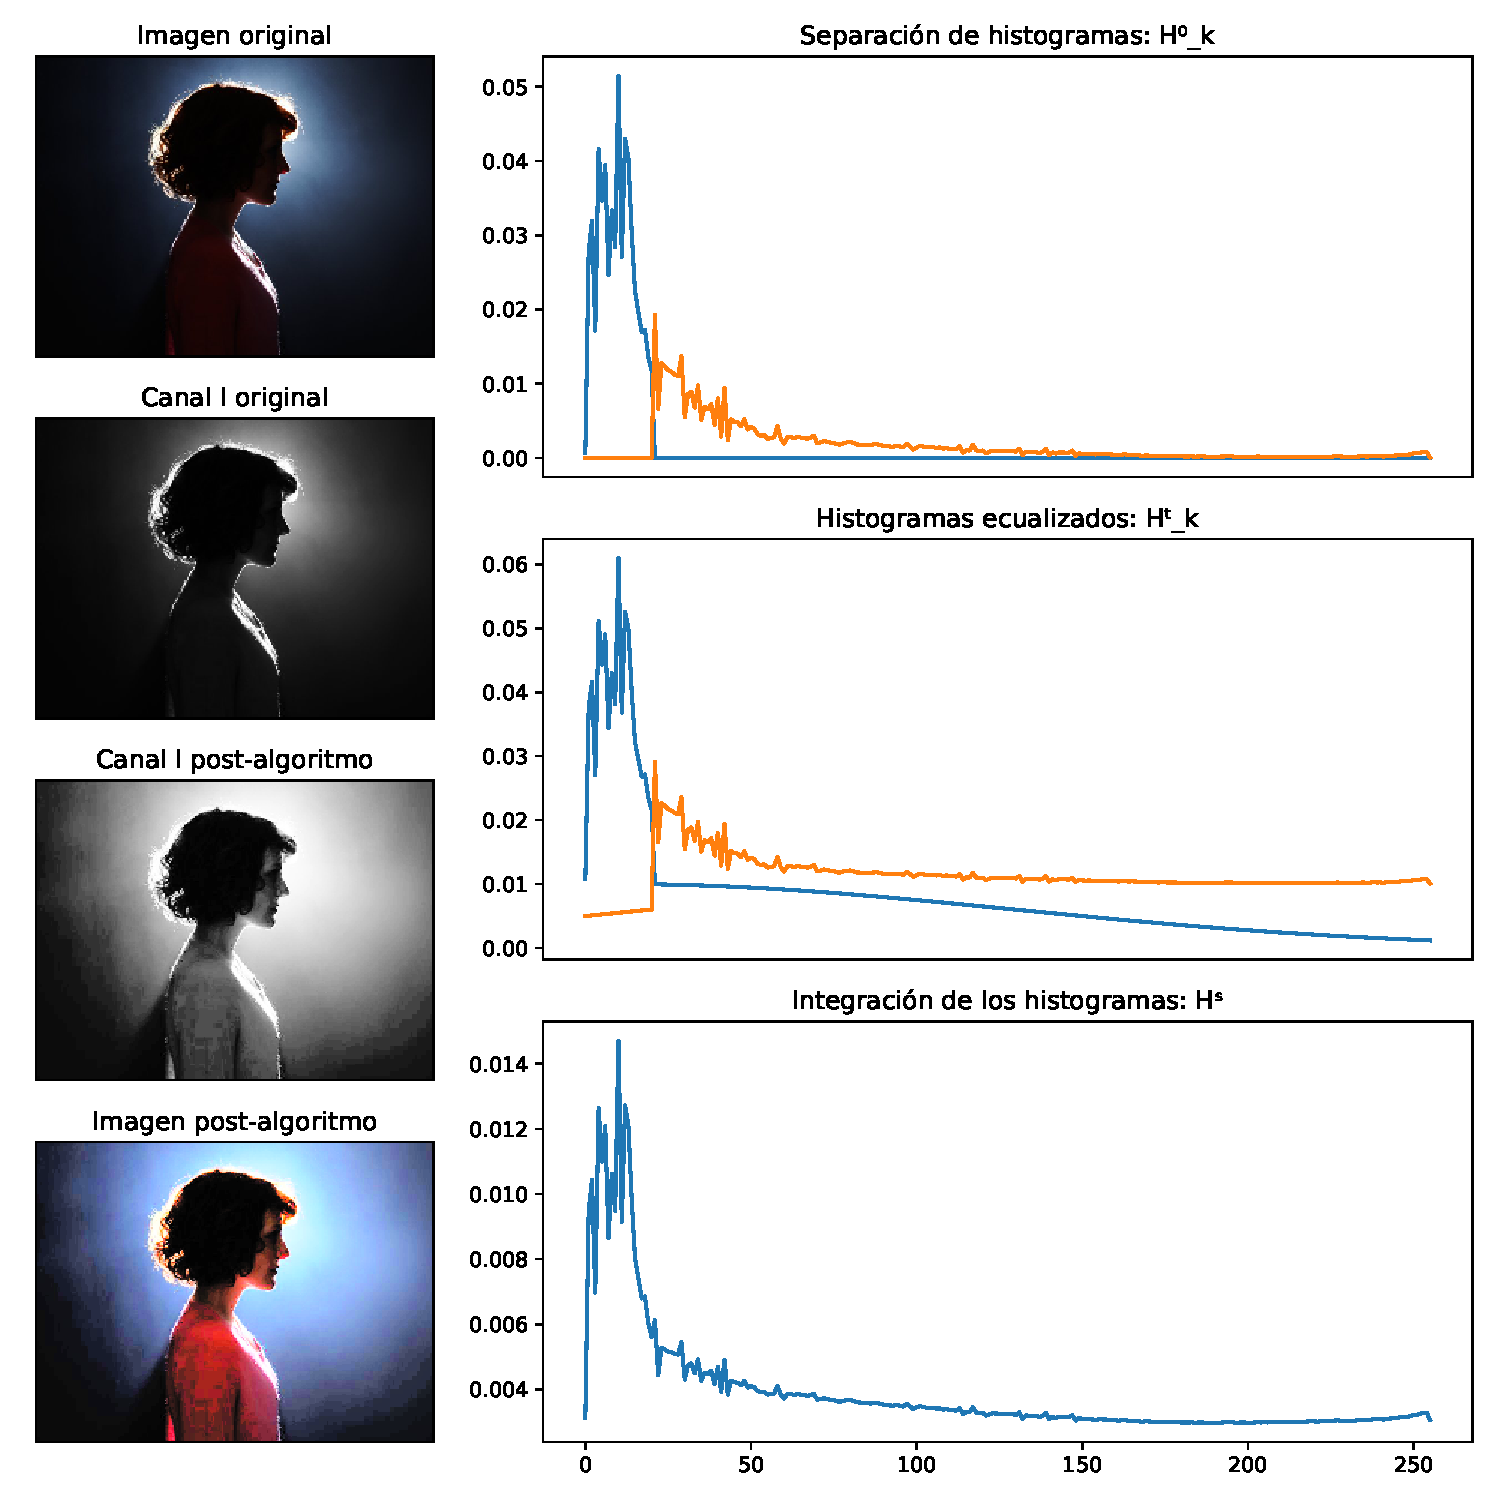
\includegraphics[height=9cm]{imgs/wom-99-01-0.pdf}
  \caption{$\alpha = 0.99, \beta = 0.01, \gamma = 0$}
\end{minipage}%
\end{figure}

\begin{figure}[H]
\begin{minipage}[c]{0.48\linewidth}
  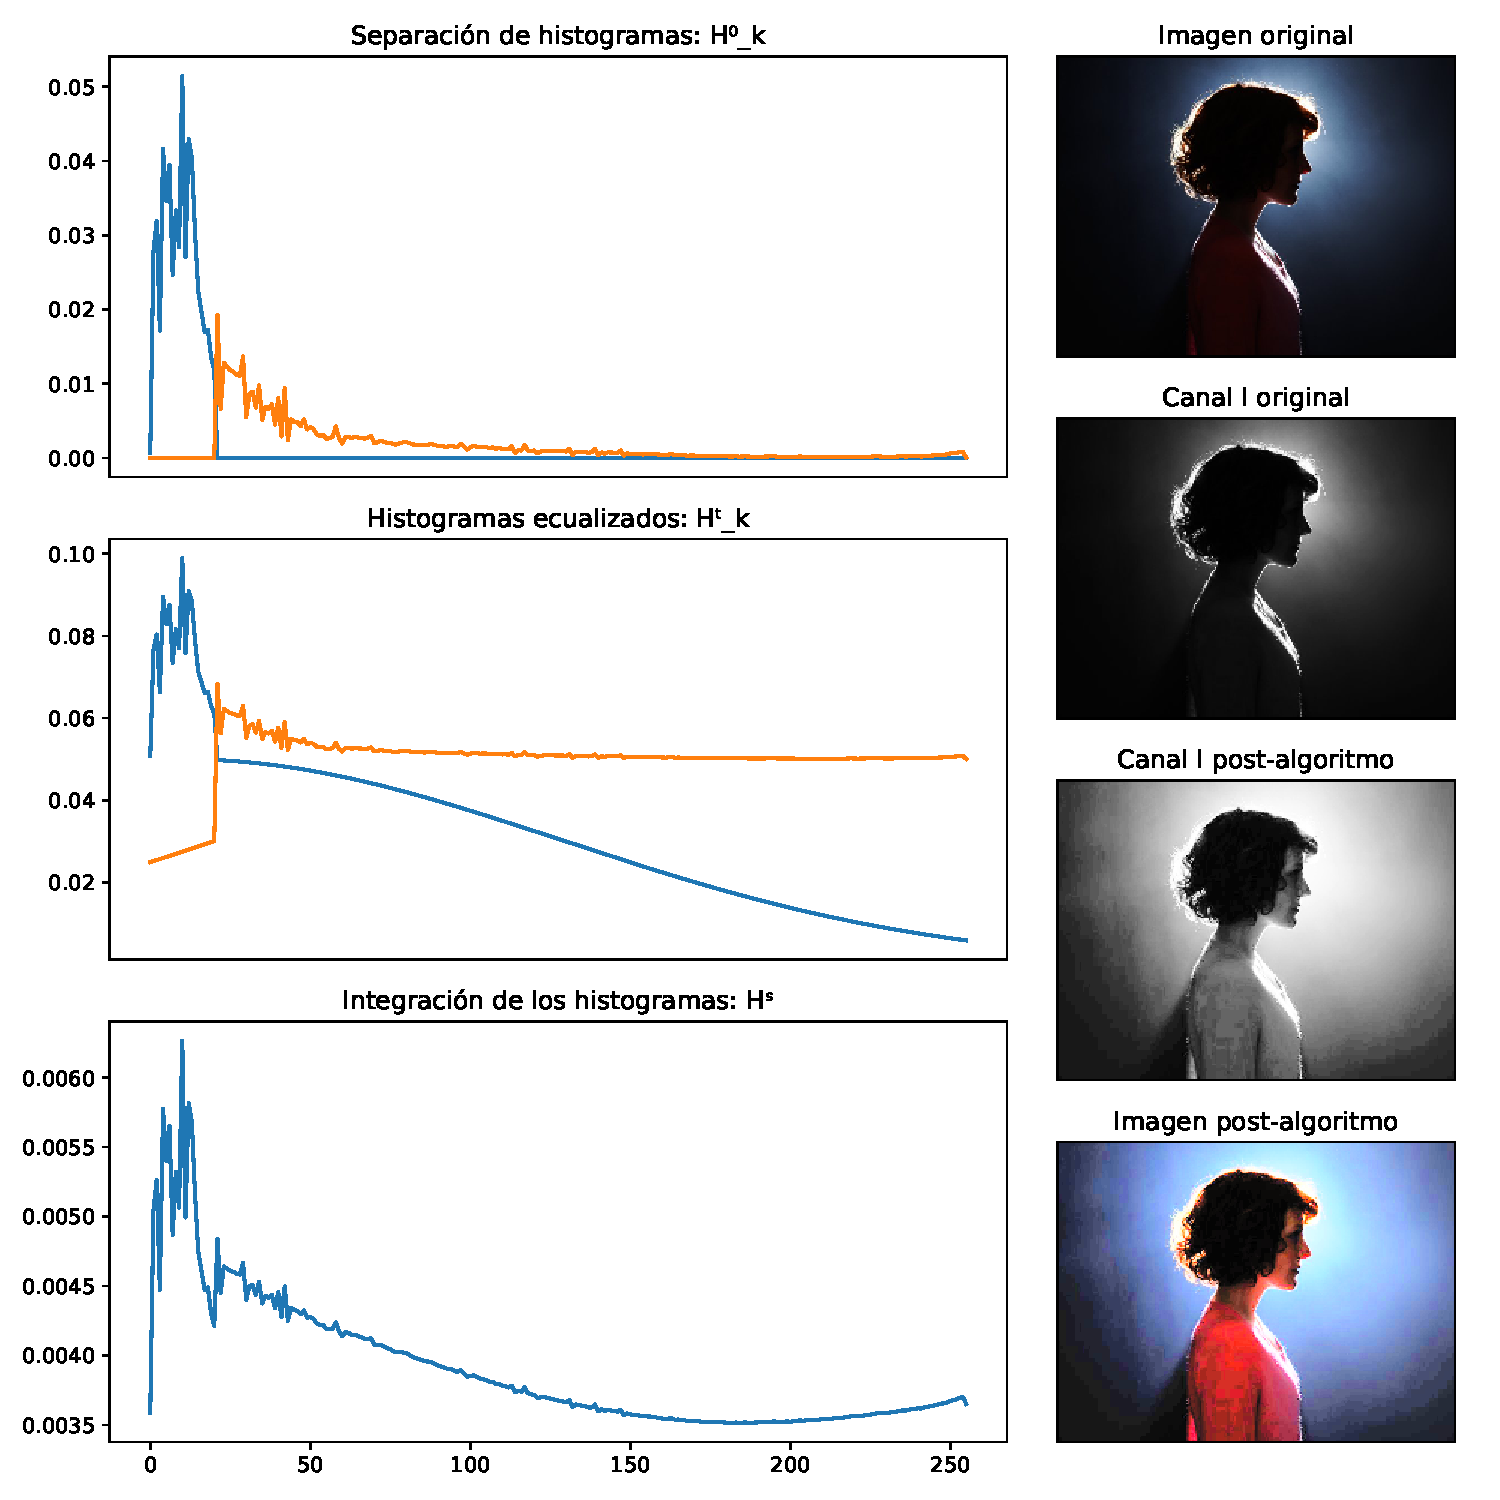
\includegraphics[height=9cm]{imgs/wom-95-05-0.pdf}
  \caption{$\alpha = 0.95, \beta = 0.05, \gamma = 0$}
\end{minipage}
\hfill
\begin{minipage}[c]{0.48\linewidth}
  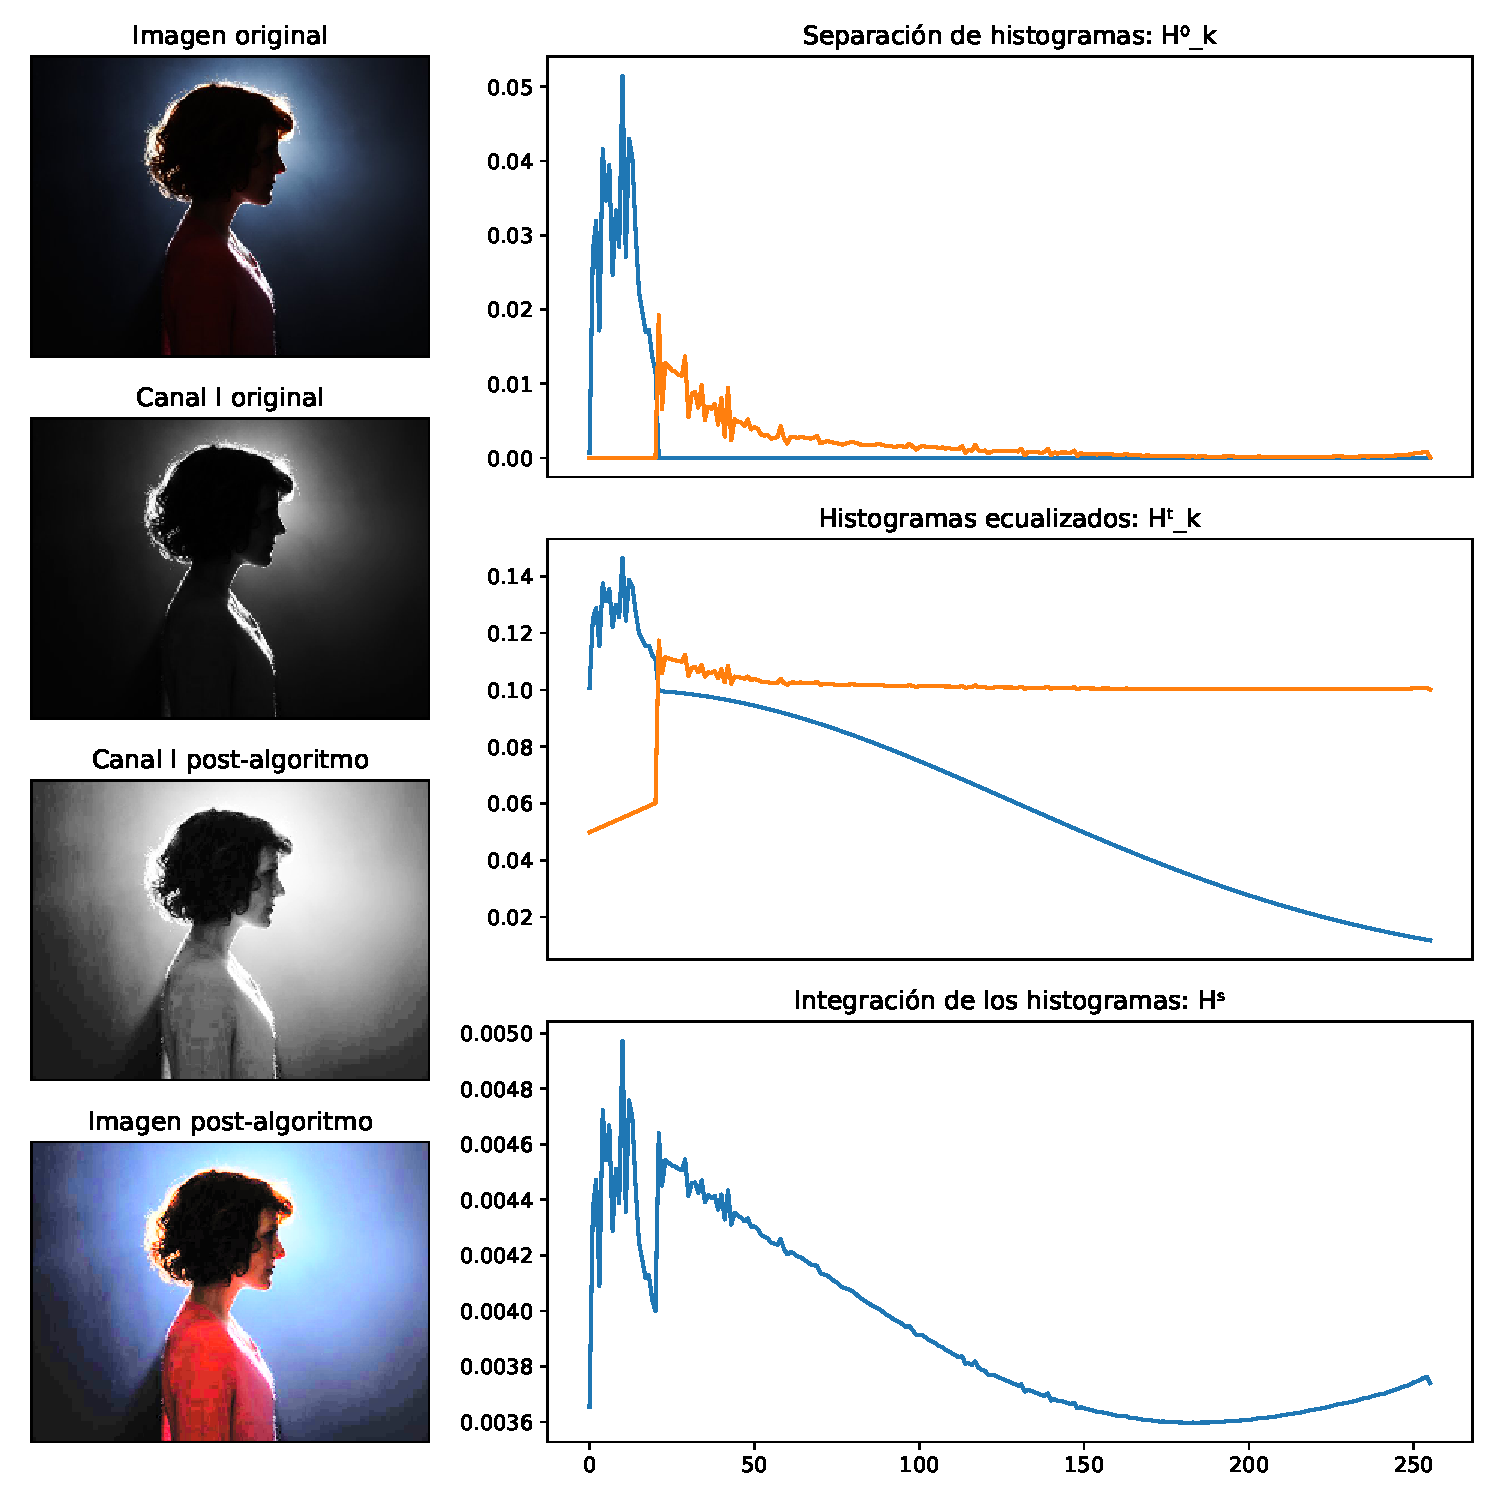
\includegraphics[height=9cm]{imgs/wom-9-1-0.pdf}
  \caption{$\alpha = 0.9, \beta = 0.1, \gamma = 0$}
\end{minipage}%
\end{figure}

\begin{figure}[H]
\begin{minipage}[c]{0.48\linewidth}
  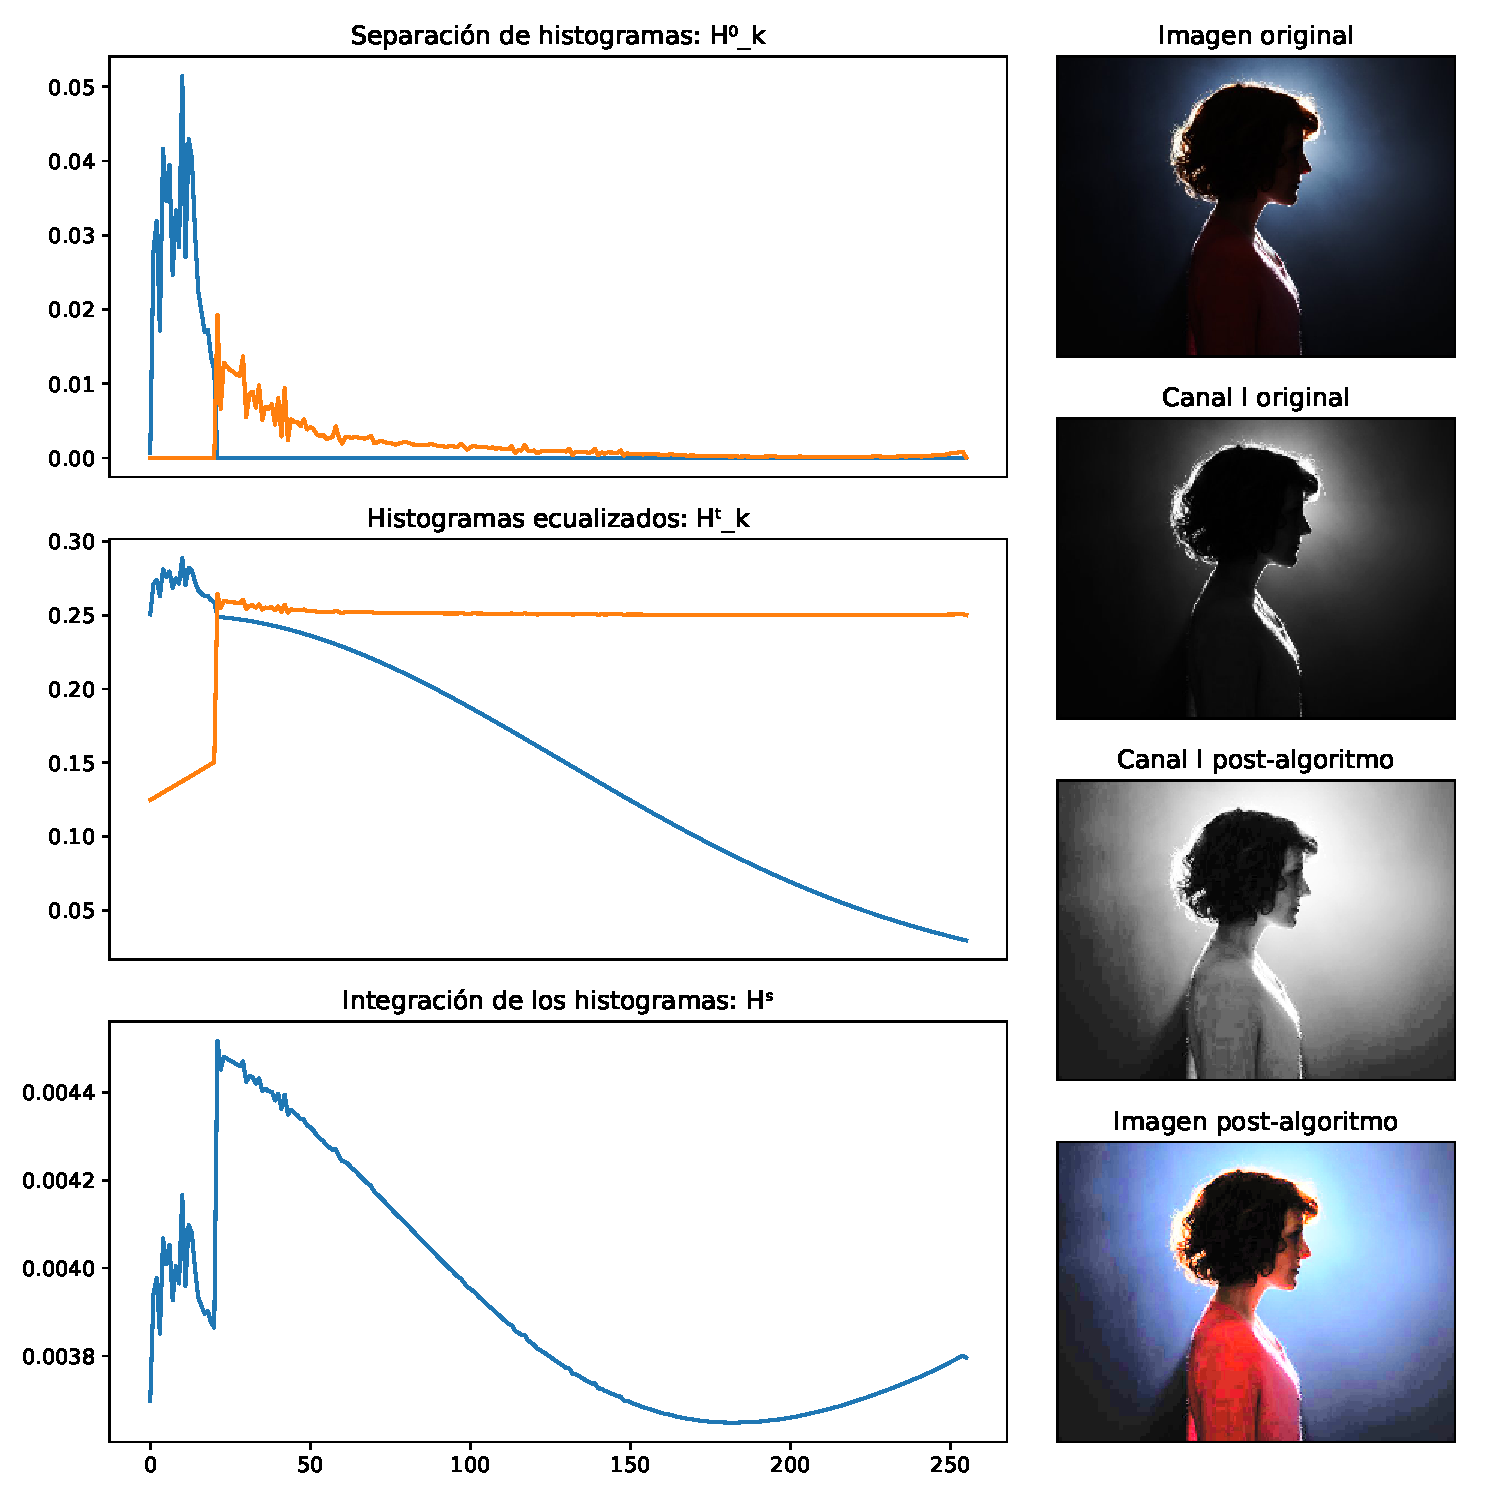
\includegraphics[height=9cm]{imgs/wom-75-25-0.pdf}
  \caption{$\alpha = 0.75, \beta = 0.25, \gamma = 0$}
\end{minipage}
\hfill
\begin{minipage}[c]{0.48\linewidth}
  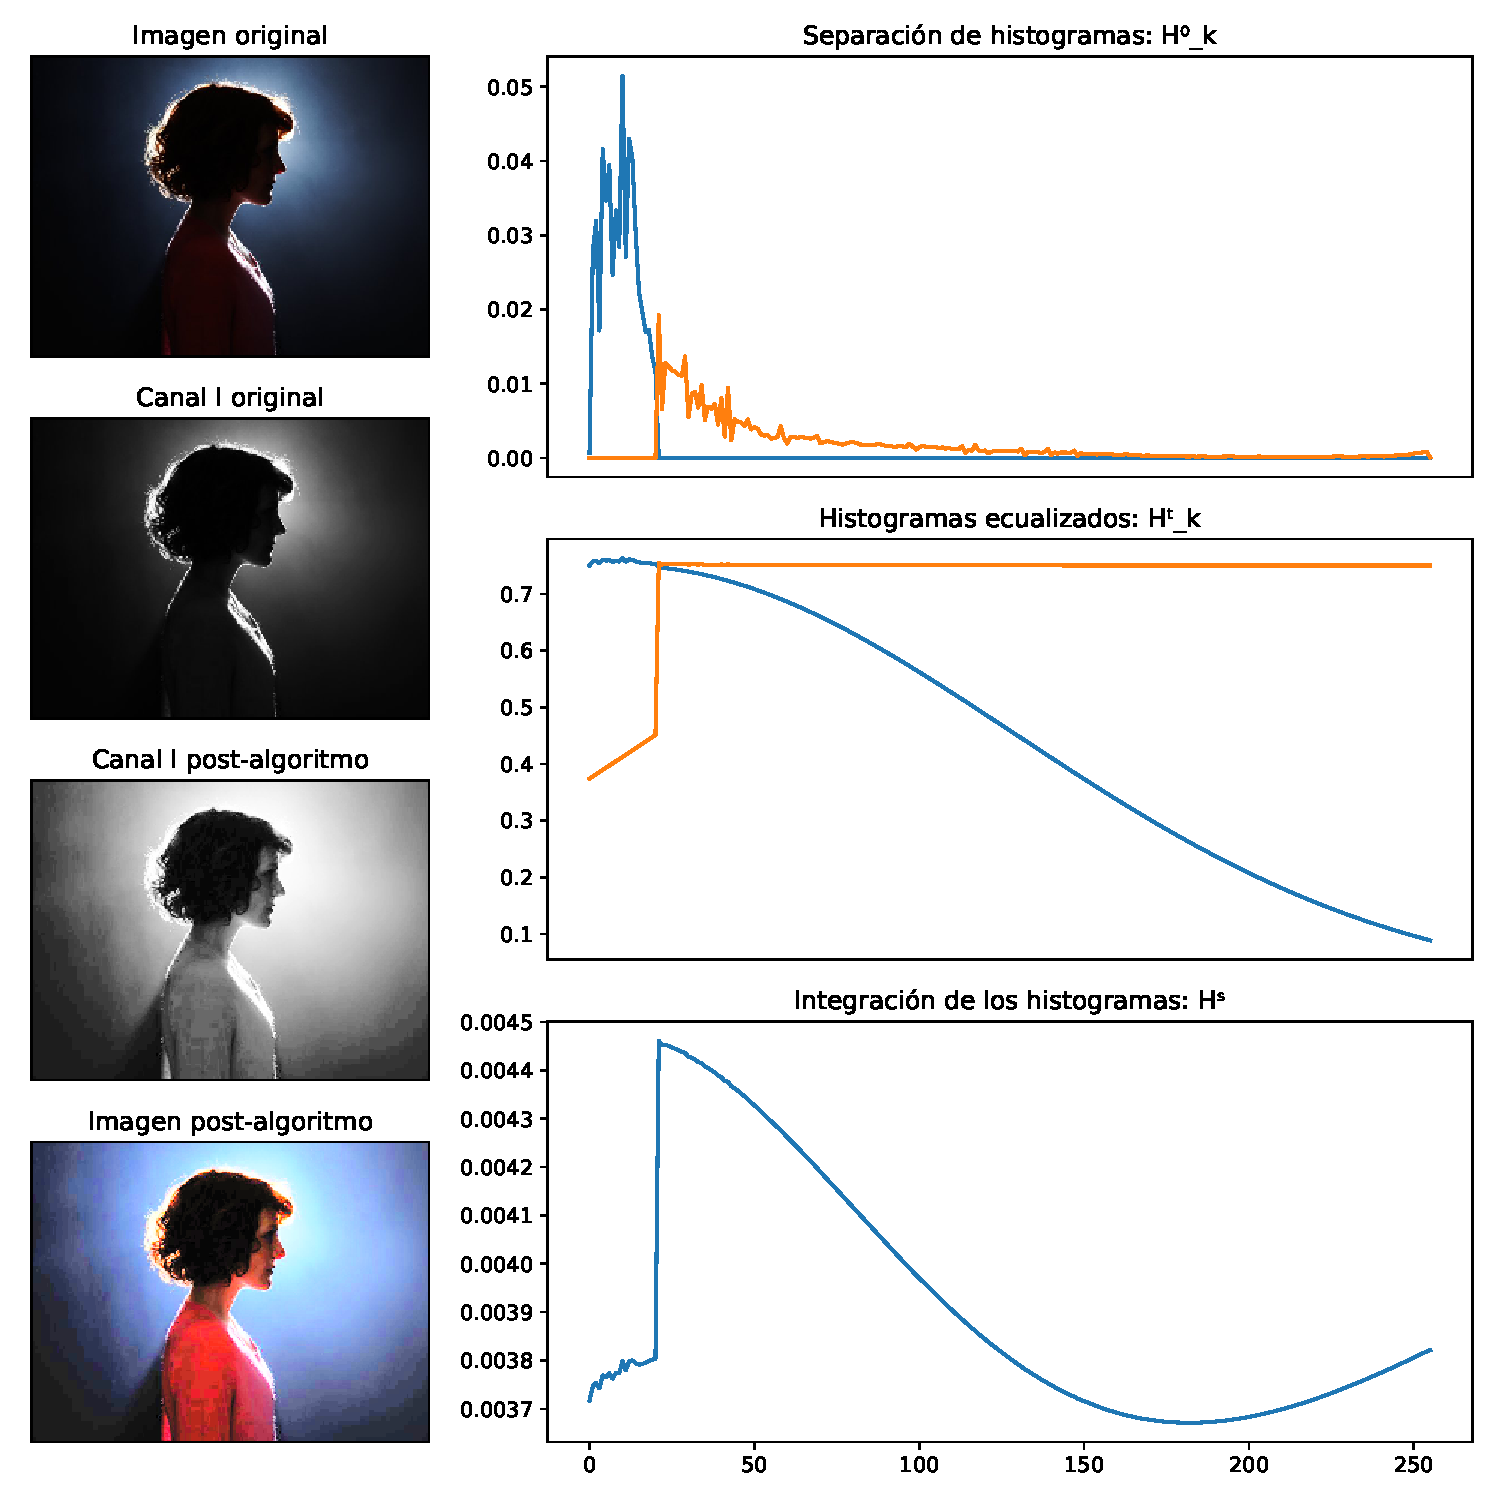
\includegraphics[height=9cm]{imgs/wom-25-75-0.pdf}
  \caption{$\alpha = 0.25, \beta = 0.75, \gamma = 0$}
\end{minipage}%
\end{figure}

\begin{figure}[H]
\begin{minipage}[c]{0.48\linewidth}
  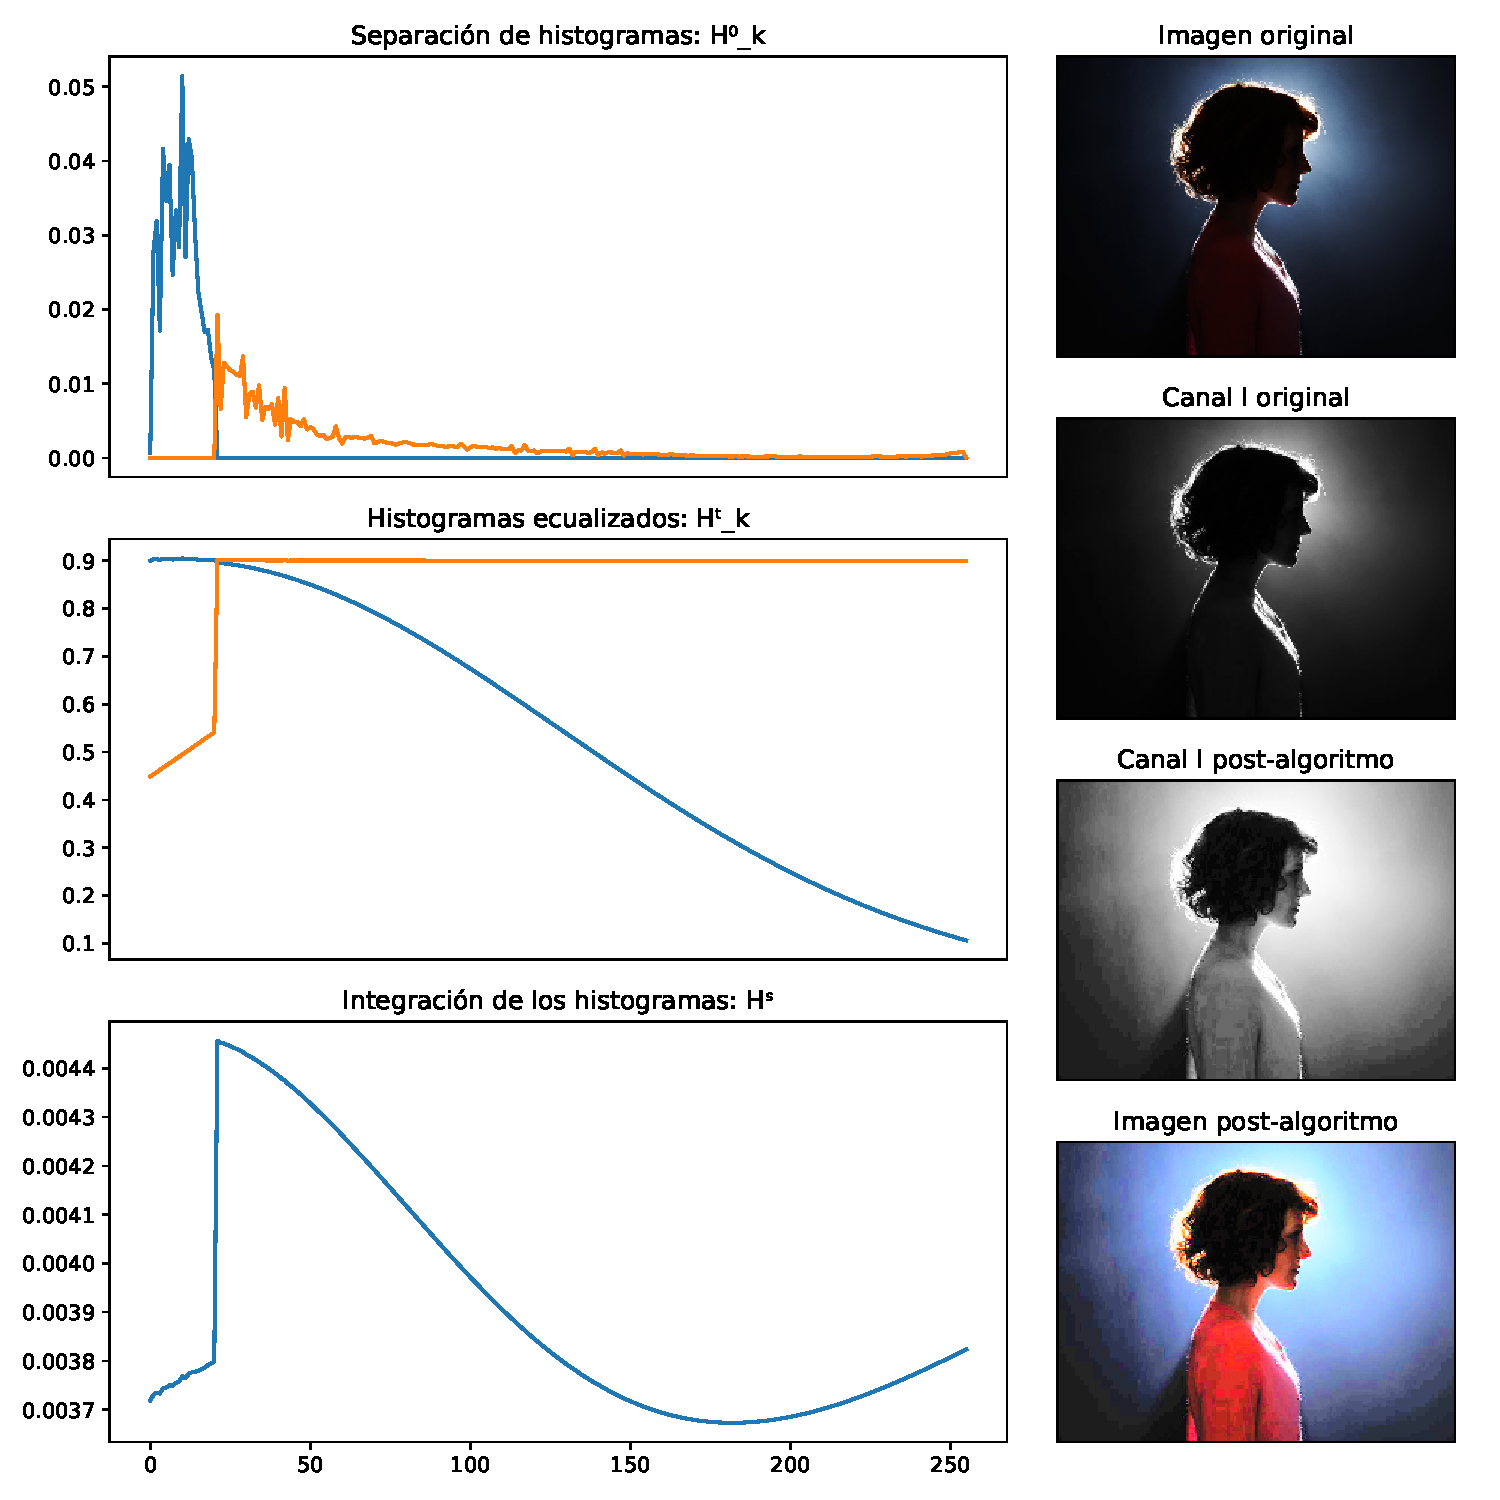
\includegraphics[height=9cm]{imgs/wom-1-9-0.pdf}
  \caption{$\alpha = 0.1, \beta = 0.9, \gamma = 0$}
\end{minipage}
\hfill
\begin{minipage}[c]{0.48\linewidth}
  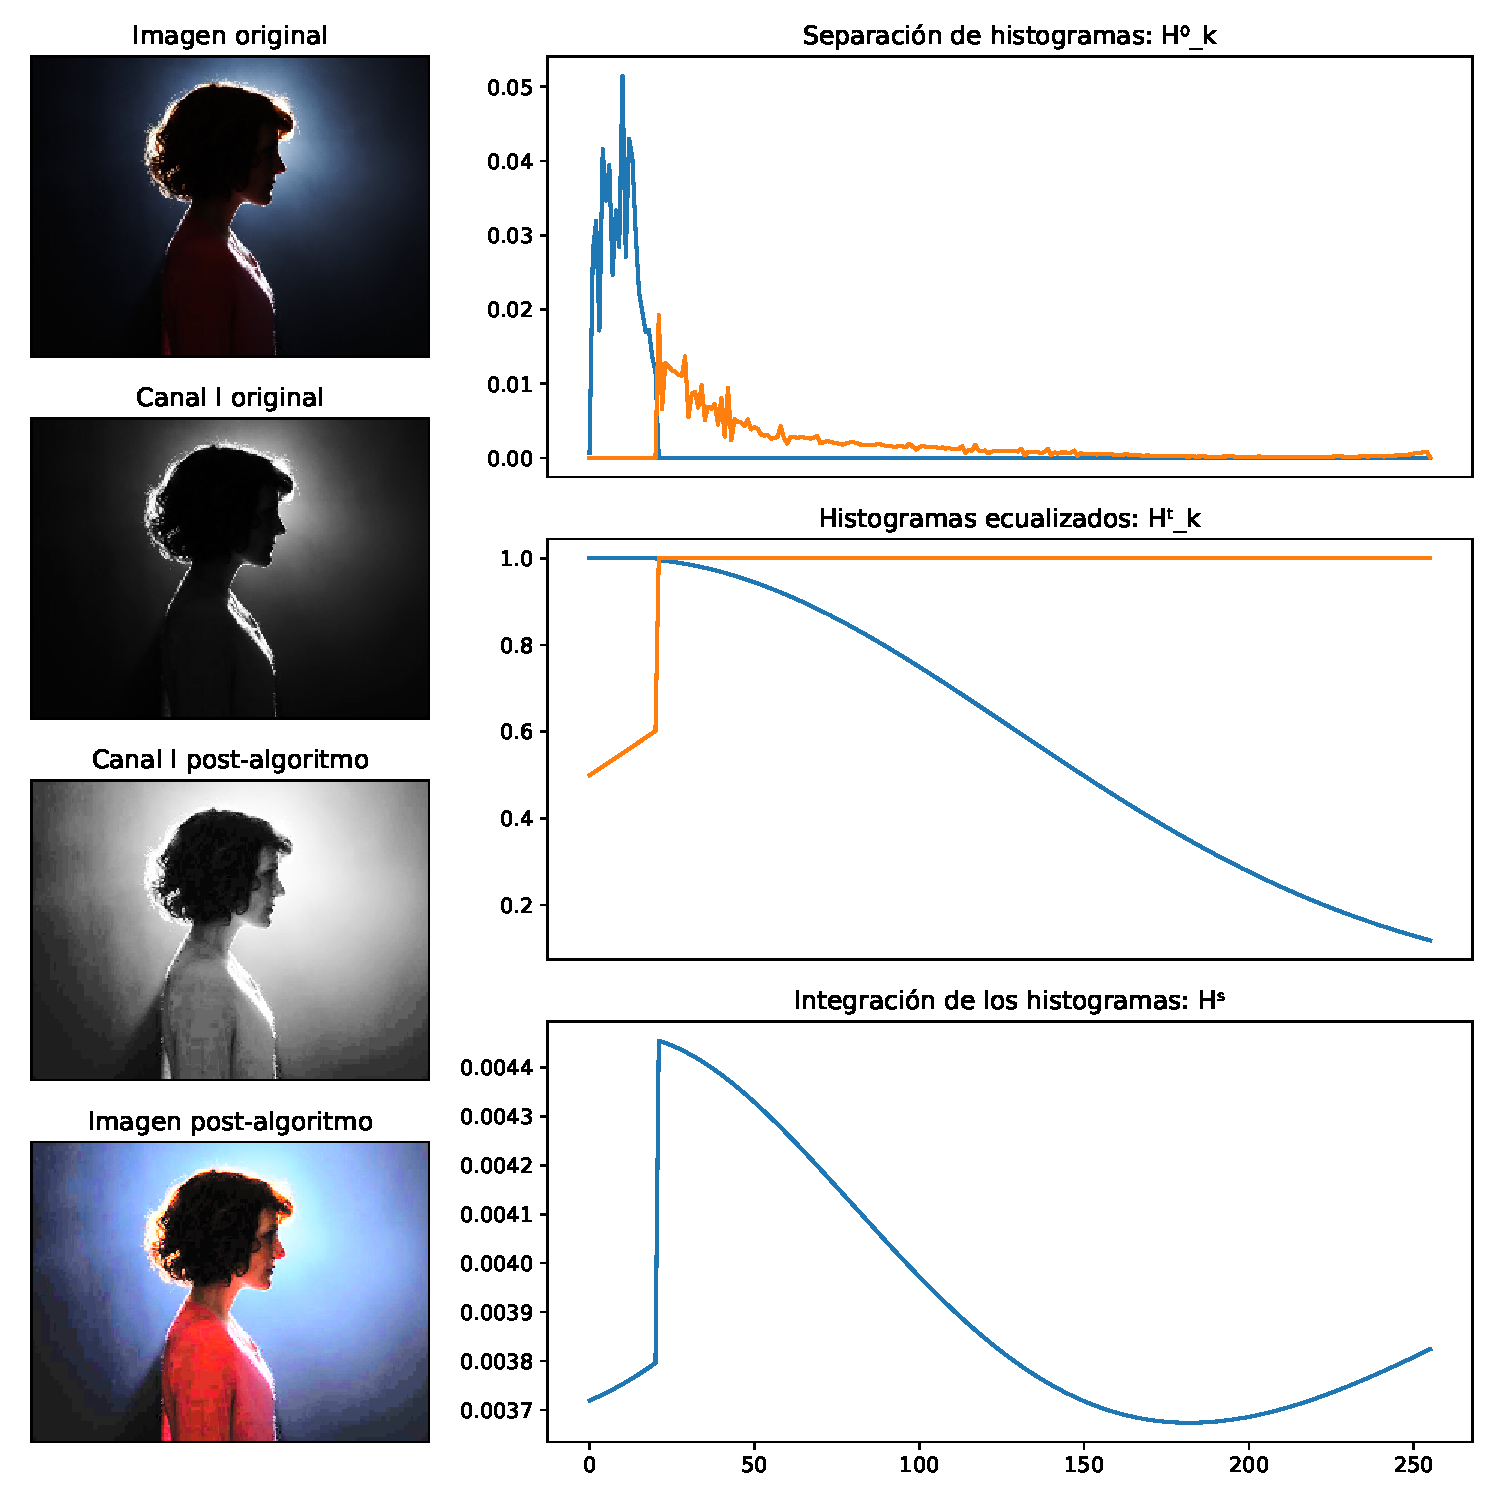
\includegraphics[height=9cm]{imgs/wom-0-1-0.pdf}
  \caption{$\alpha = 0, \beta = 1, \gamma = 0$}
\end{minipage}%
\end{figure}

\begin{figure}[H]
\begin{minipage}[c]{0.48\linewidth}
  \includegraphics[height=9cm]{imgs/porch-9-1-0.pdf}
  \caption{$\alpha = 0.9, \beta = 0.1, \gamma = 0$}
\end{minipage}
\hfill
\begin{minipage}[c]{0.48\linewidth}
  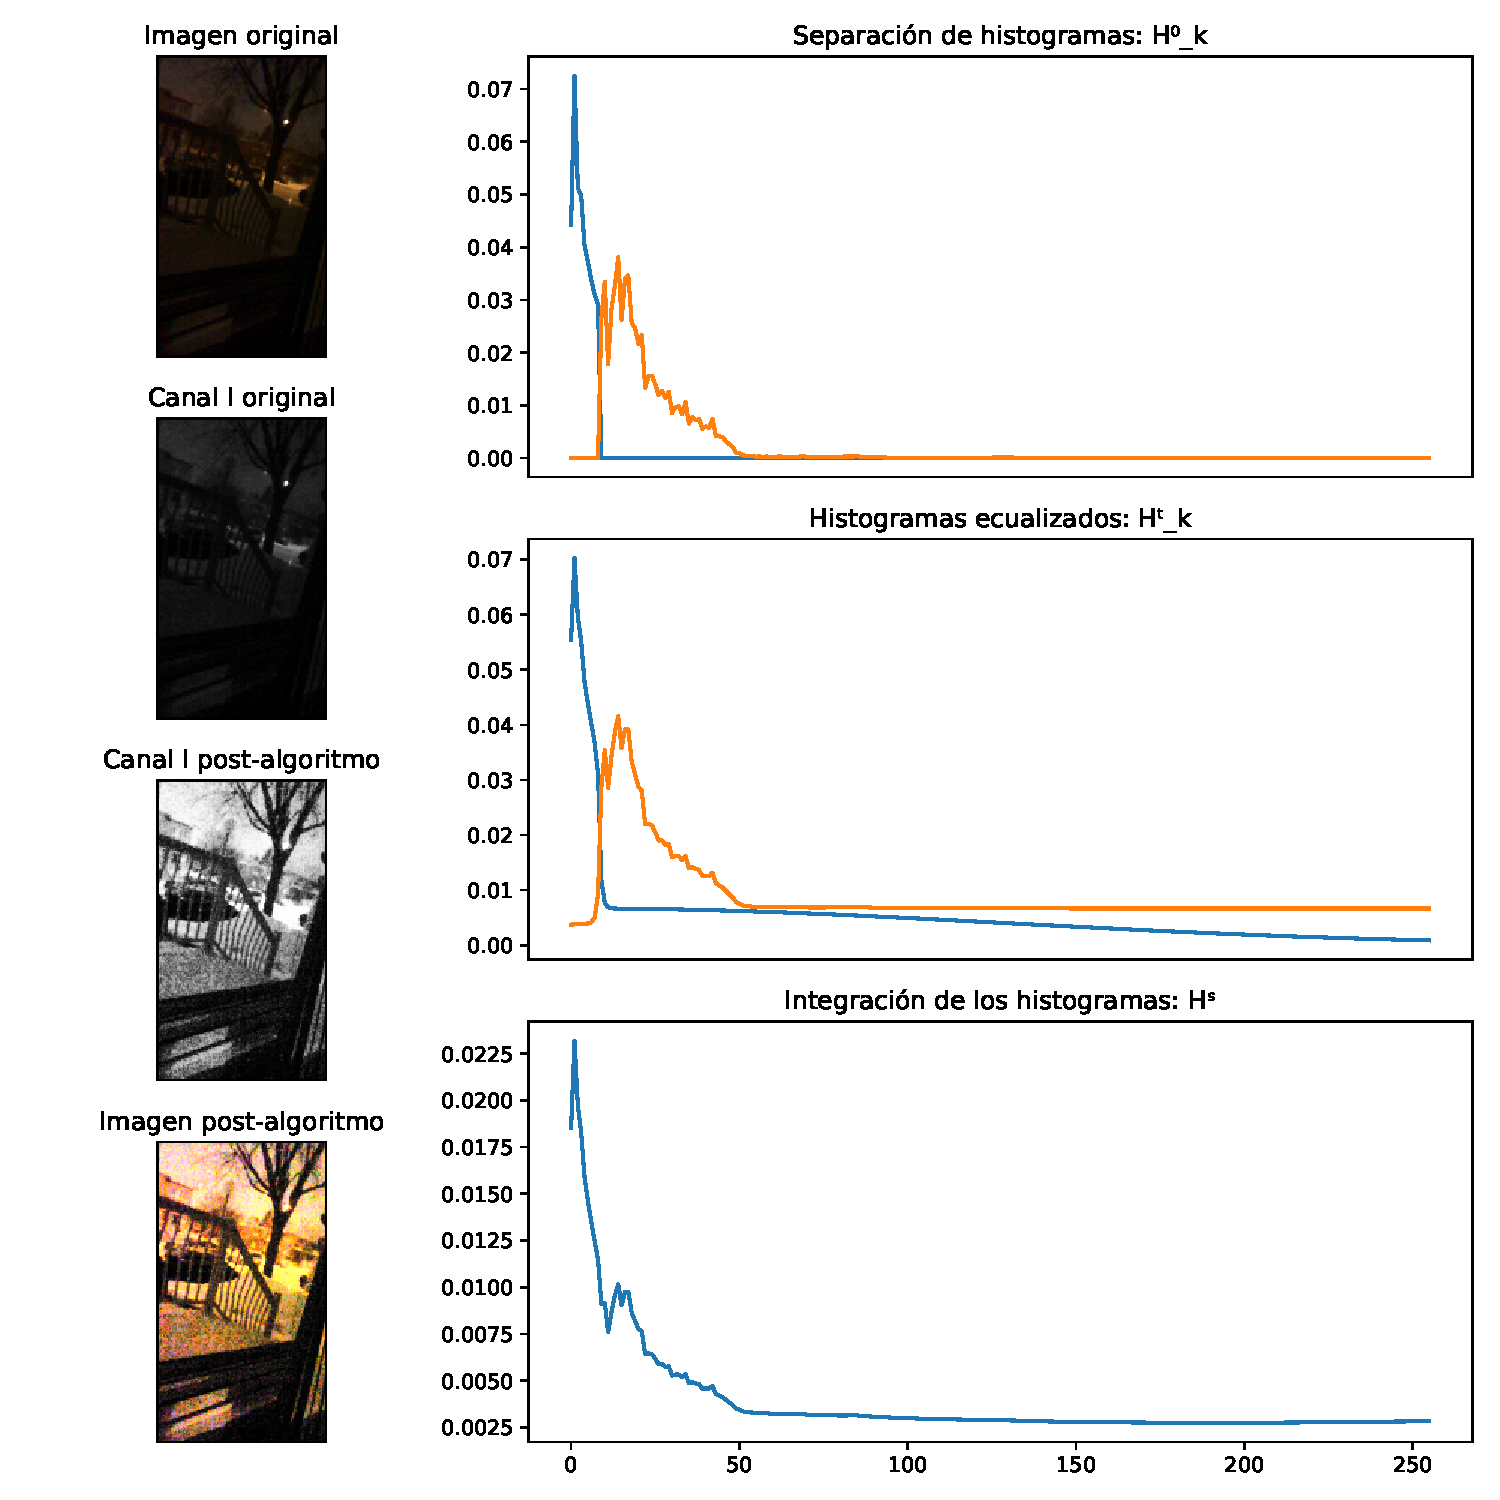
\includegraphics[height=9cm]{imgs/porch-745-005-25.pdf}
  \caption{$\alpha = 0.745, \beta = 0.005, \gamma = 0.25$}
\end{minipage}%
\end{figure}

\begin{figure}[H]
\begin{minipage}[c]{0.48\linewidth}
  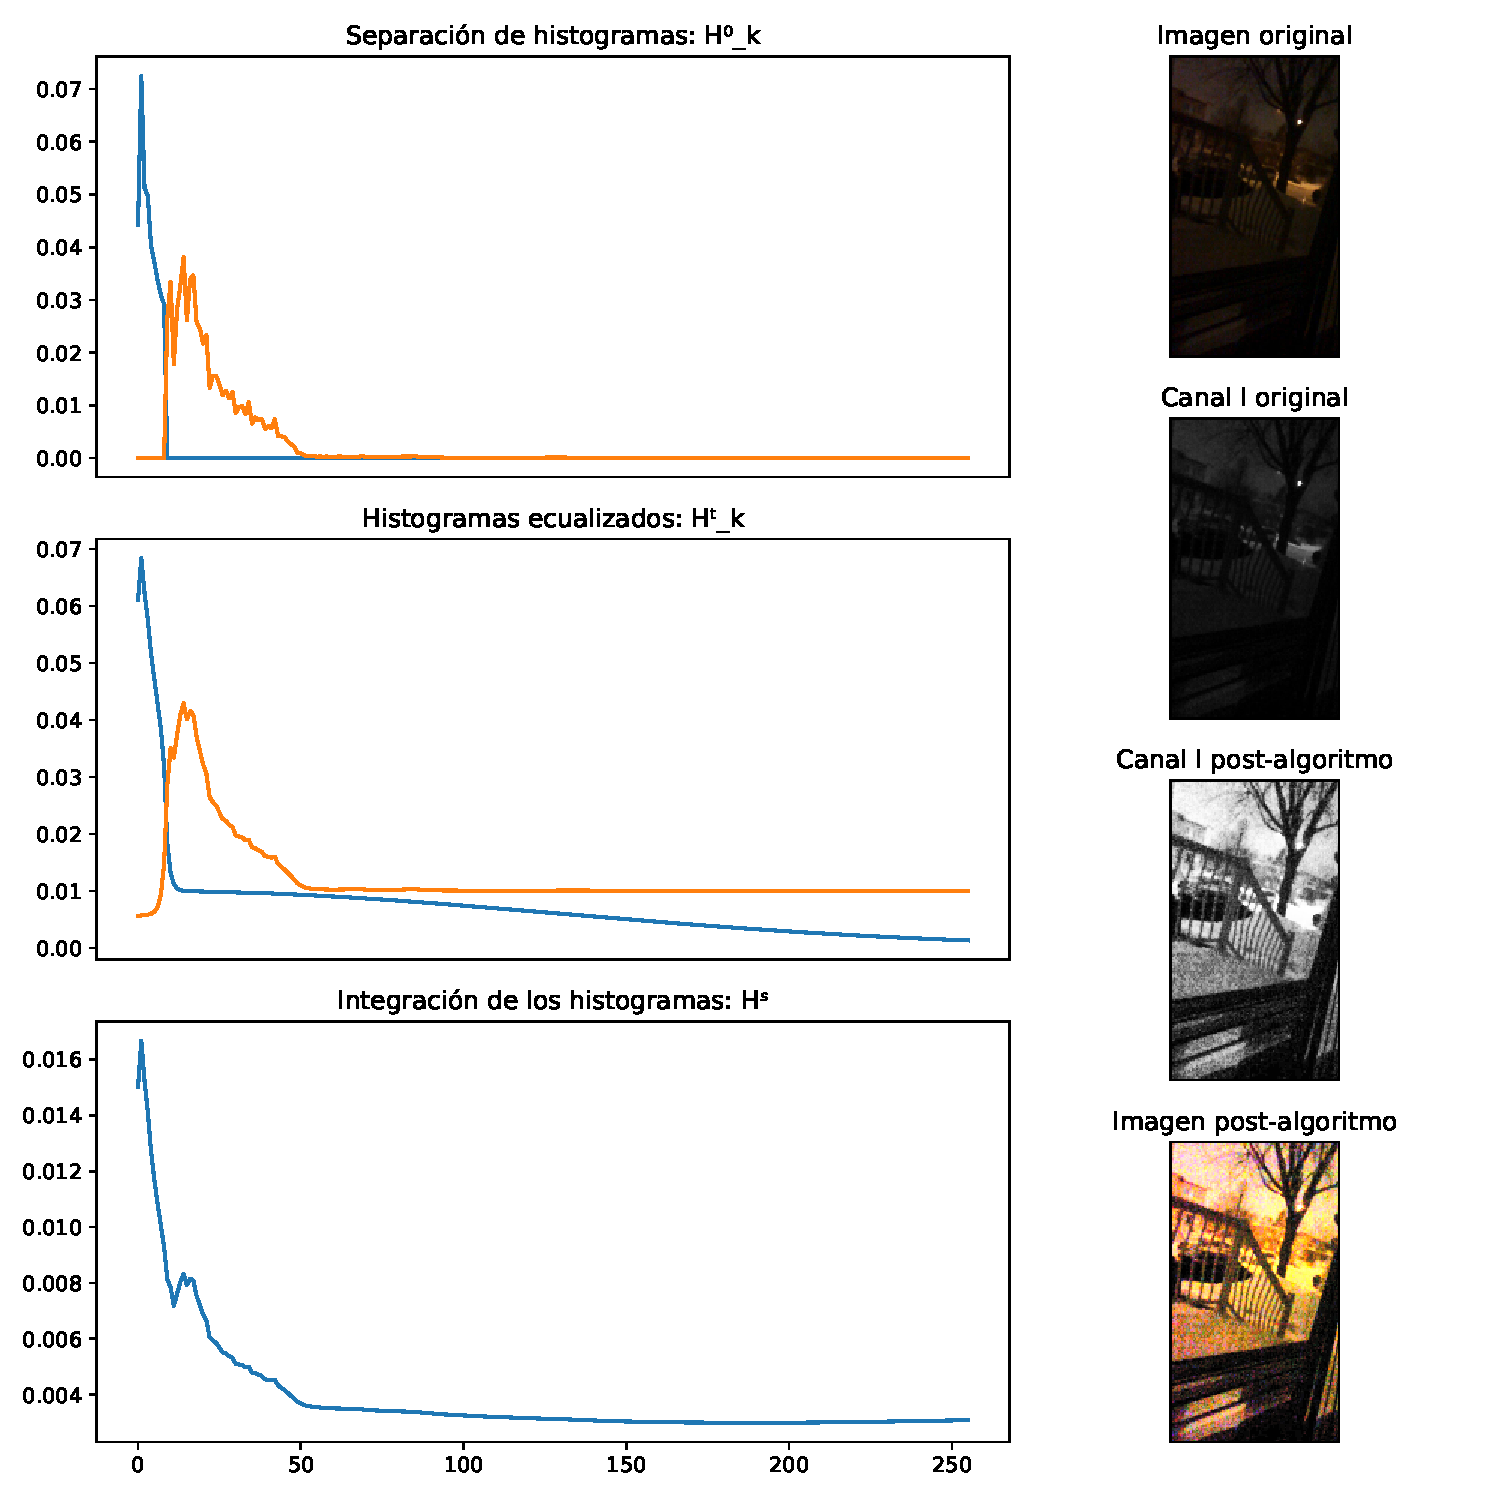
\includegraphics[height=9cm]{imgs/porch-495-005-5.pdf}
  \caption{$\alpha = 0.495, \beta = 0.005, \gamma = 0.5$}
\end{minipage}
\hfill
\begin{minipage}[c]{0.48\linewidth}
  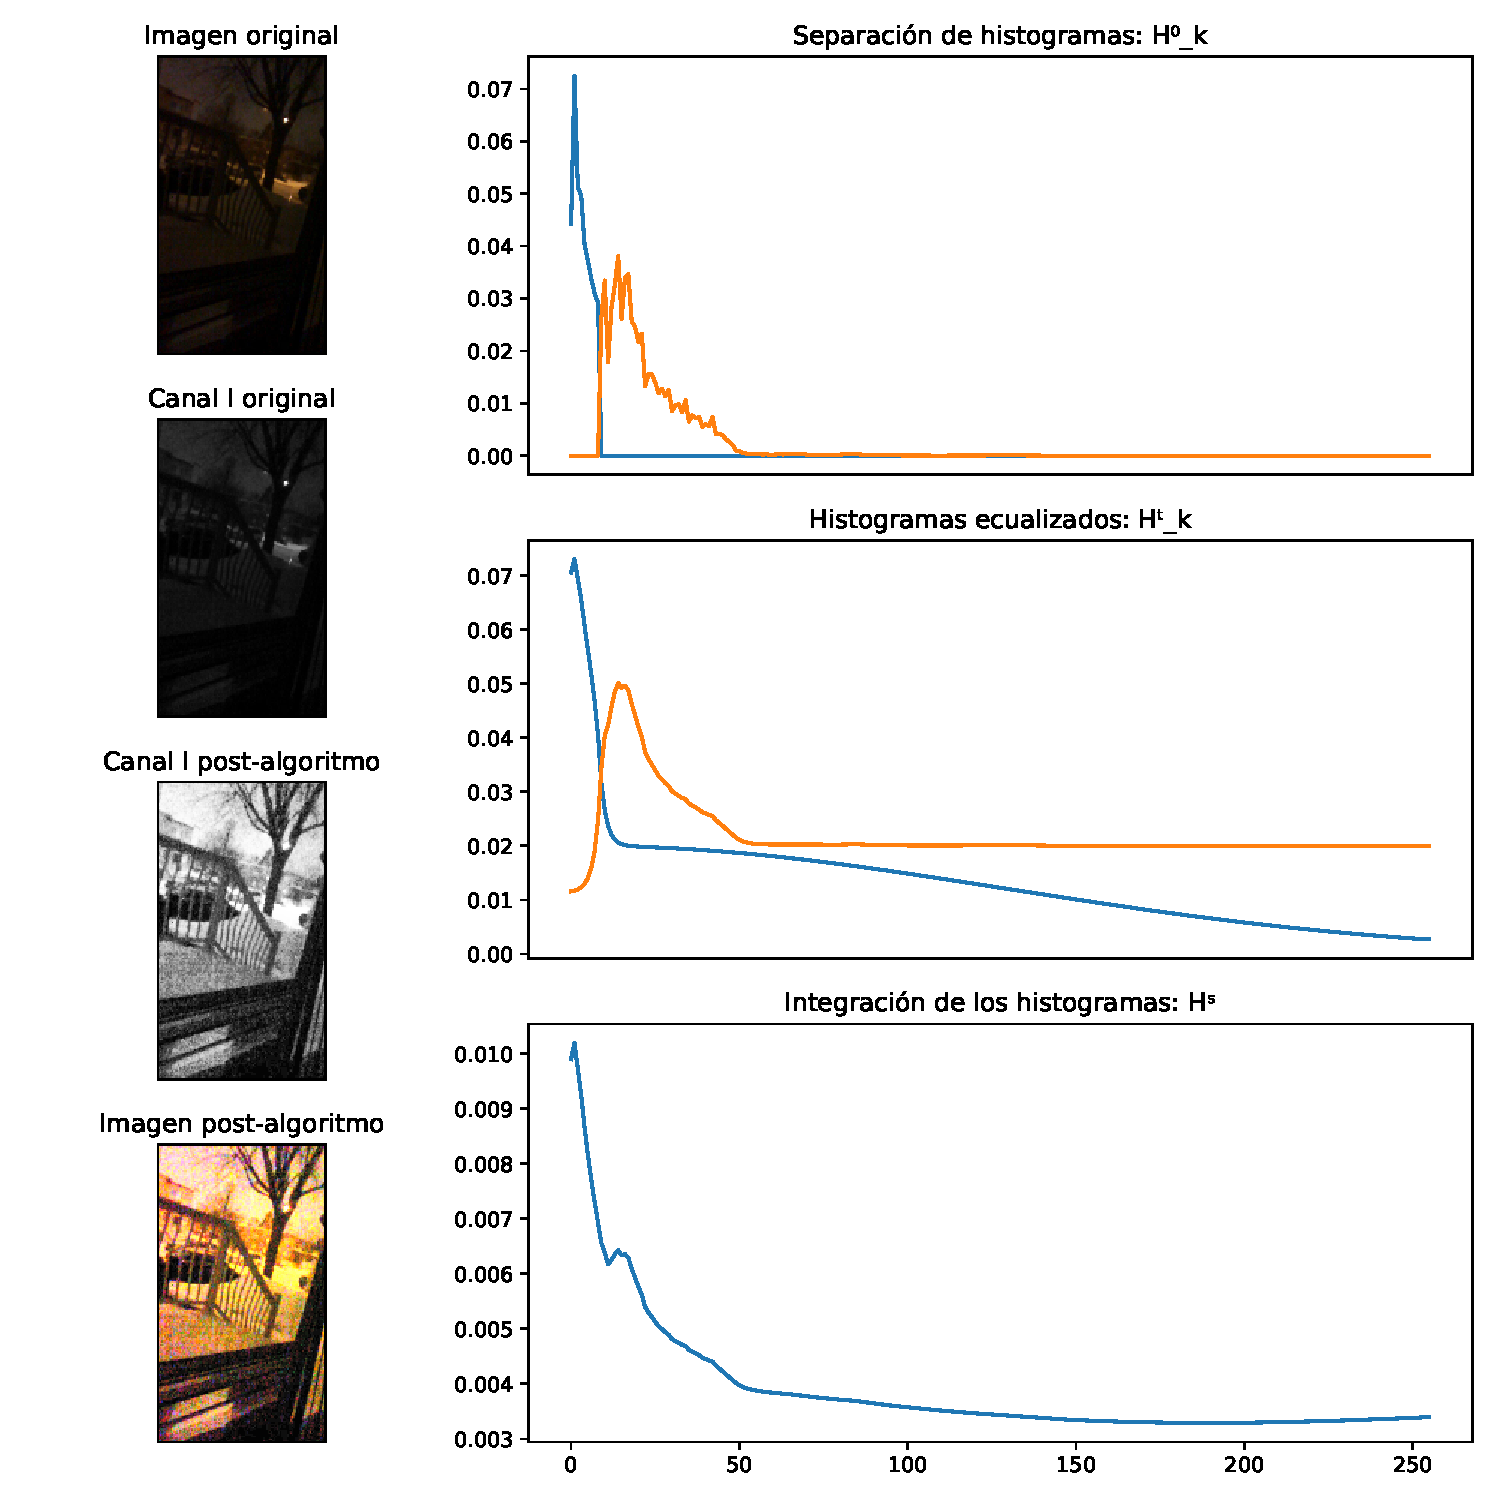
\includegraphics[height=9cm]{imgs/porch-245-005-75.pdf}
  \caption{$\alpha = 0.245, \beta = 0.005, \gamma = 0.75$}
\end{minipage}%
\end{figure}

\begin{figure}[H]
\begin{minipage}[c]{0.48\linewidth}
  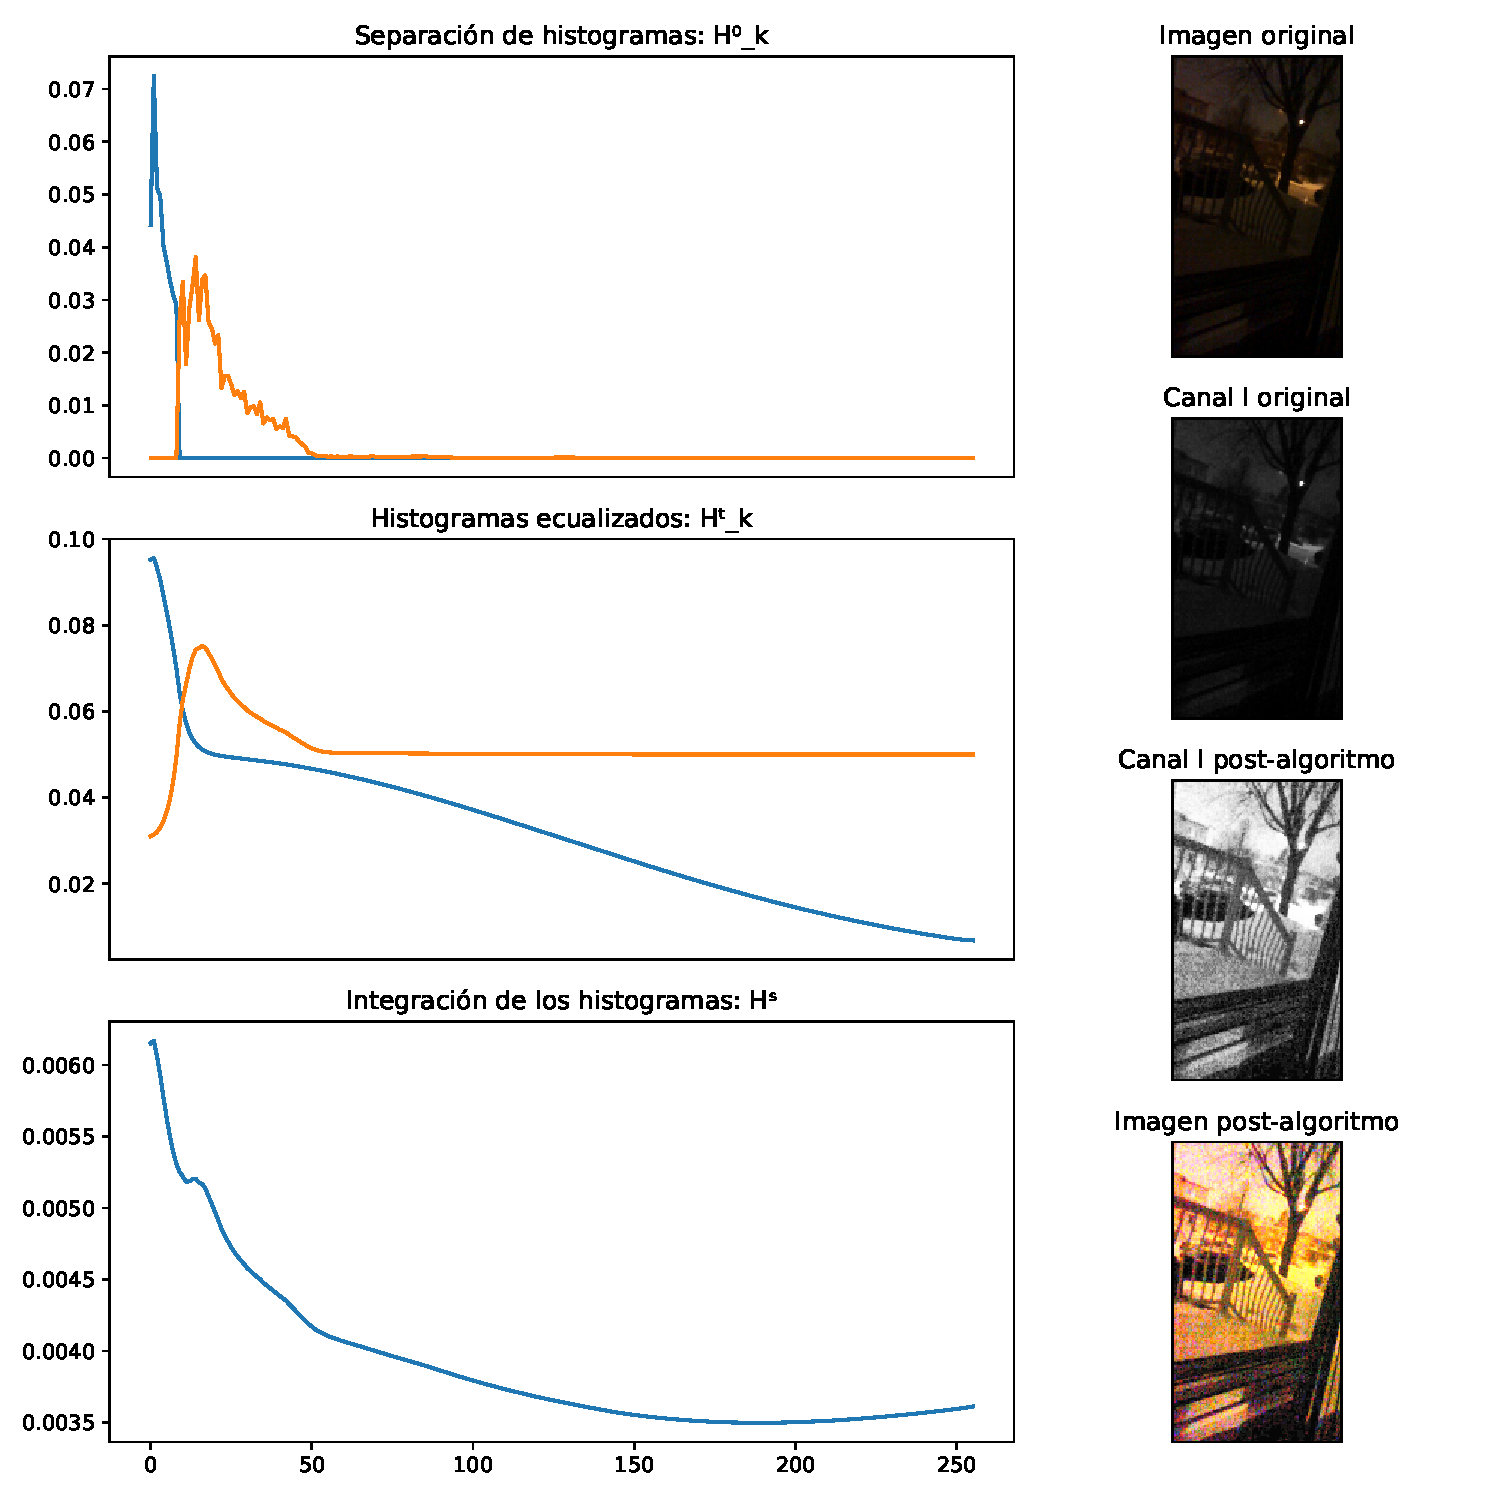
\includegraphics[height=9cm]{imgs/porch-095-005-9.pdf}
  \caption{$\alpha = 0.095, \beta = 0.005, \gamma = 0.9$}
\end{minipage}
\hfill
\begin{minipage}[c]{0.48\linewidth}
  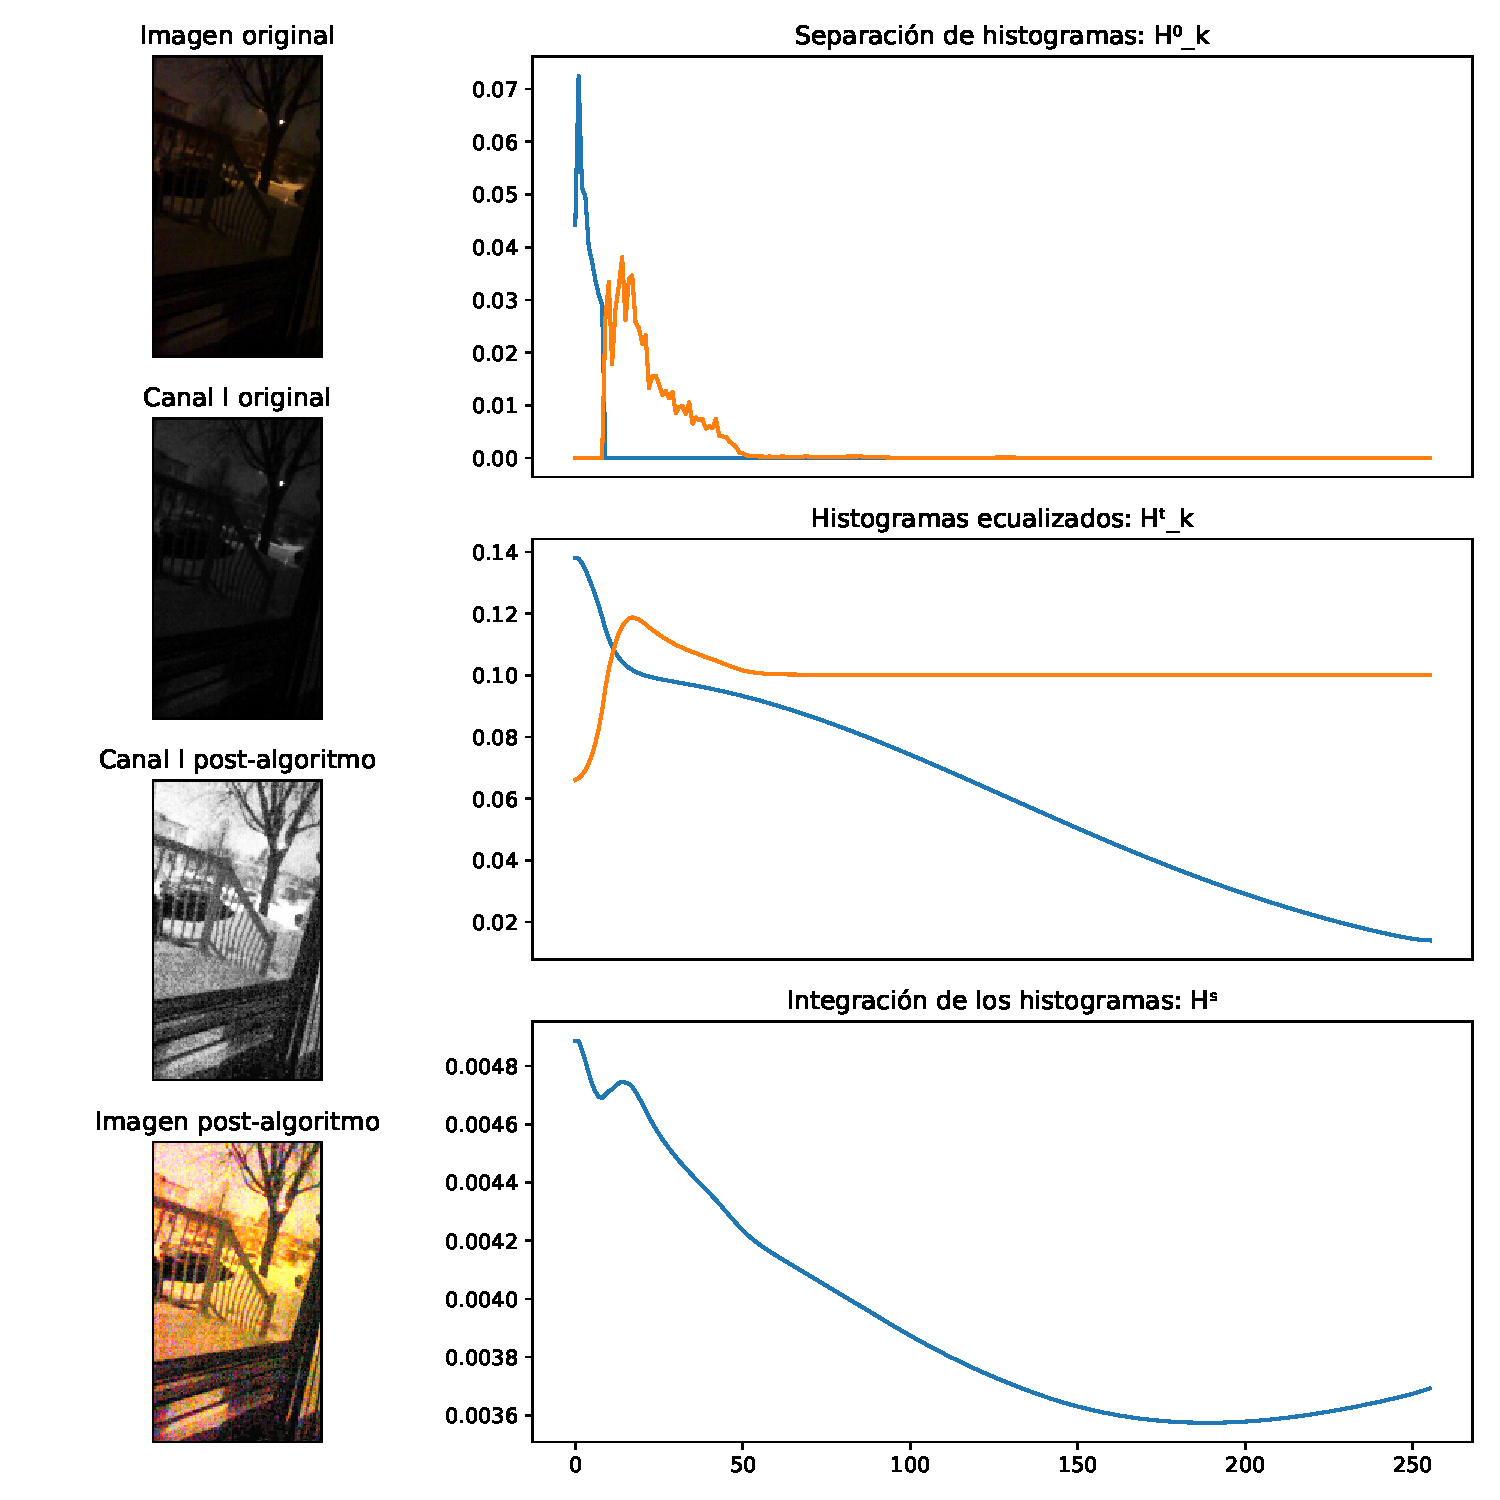
\includegraphics[height=9cm]{imgs/porch-045-005-95.pdf}
  \caption{$\alpha = 0.045, \beta = 0.005, \gamma = 0.95$}
\end{minipage}%
\end{figure}


\newpage

\section{Ejemplos}

\begin{figure}[H]
\begin{minipage}[c]{0.48\linewidth}
  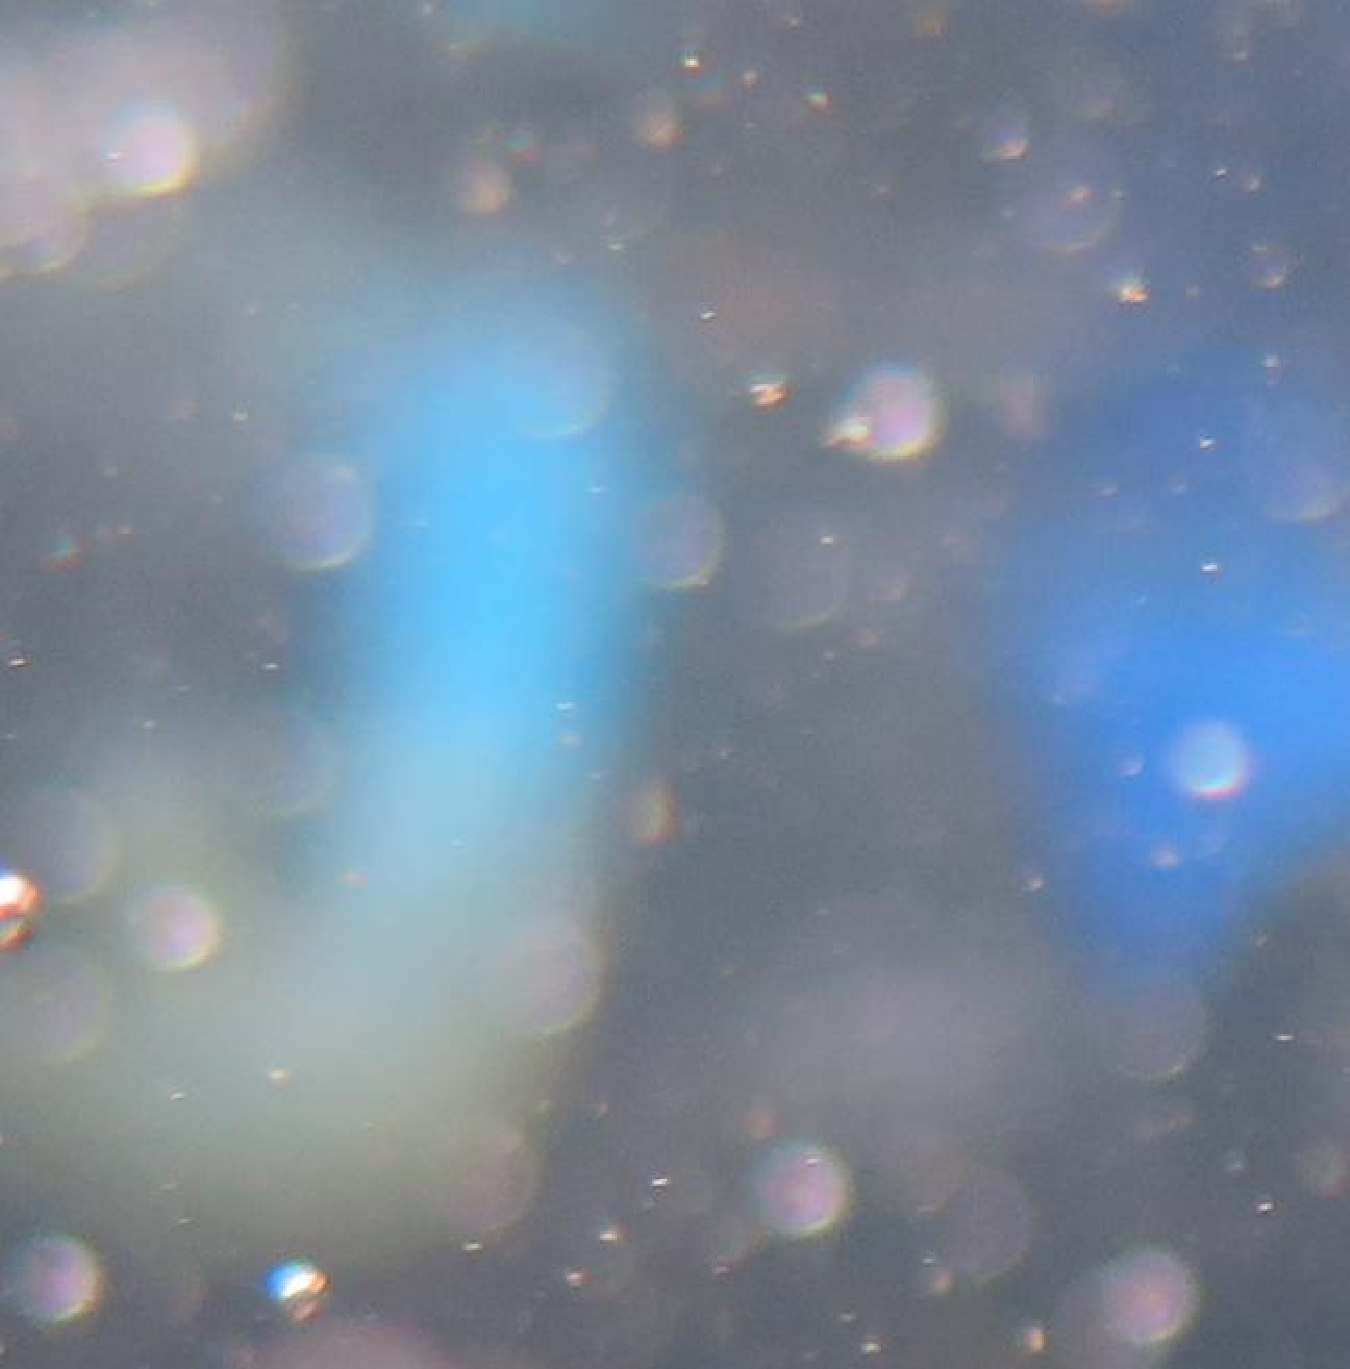
\includegraphics[height=9cm]{imgs/1923xx.pdf}
  \caption{Imagen original}
\end{minipage}
\hfill
\begin{minipage}[c]{0.48\linewidth}
  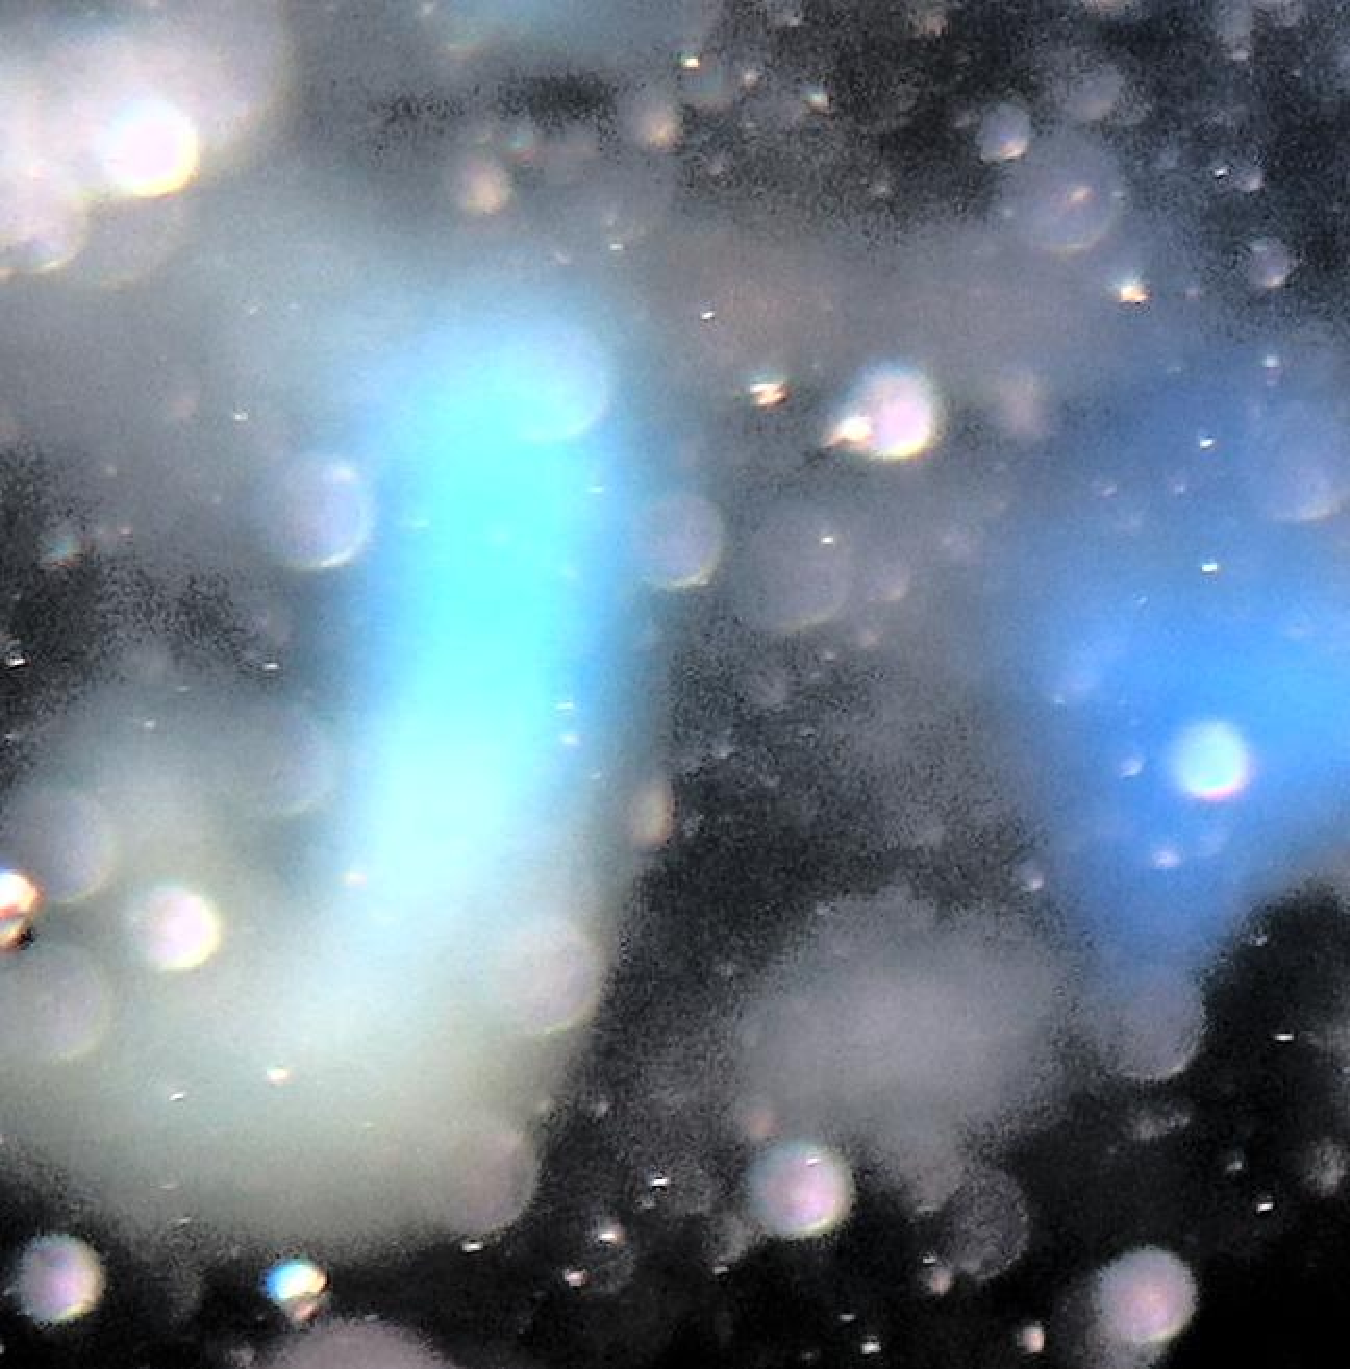
\includegraphics[height=9cm]{imgs/1923xxOut.pdf}
    \caption{$\alpha = 0.995, \beta = 0.005, \gamma = 0, [1, 1, 8]$}
\end{minipage}%
\end{figure}

\begin{figure}[H]
\begin{minipage}[c]{0.48\linewidth}
  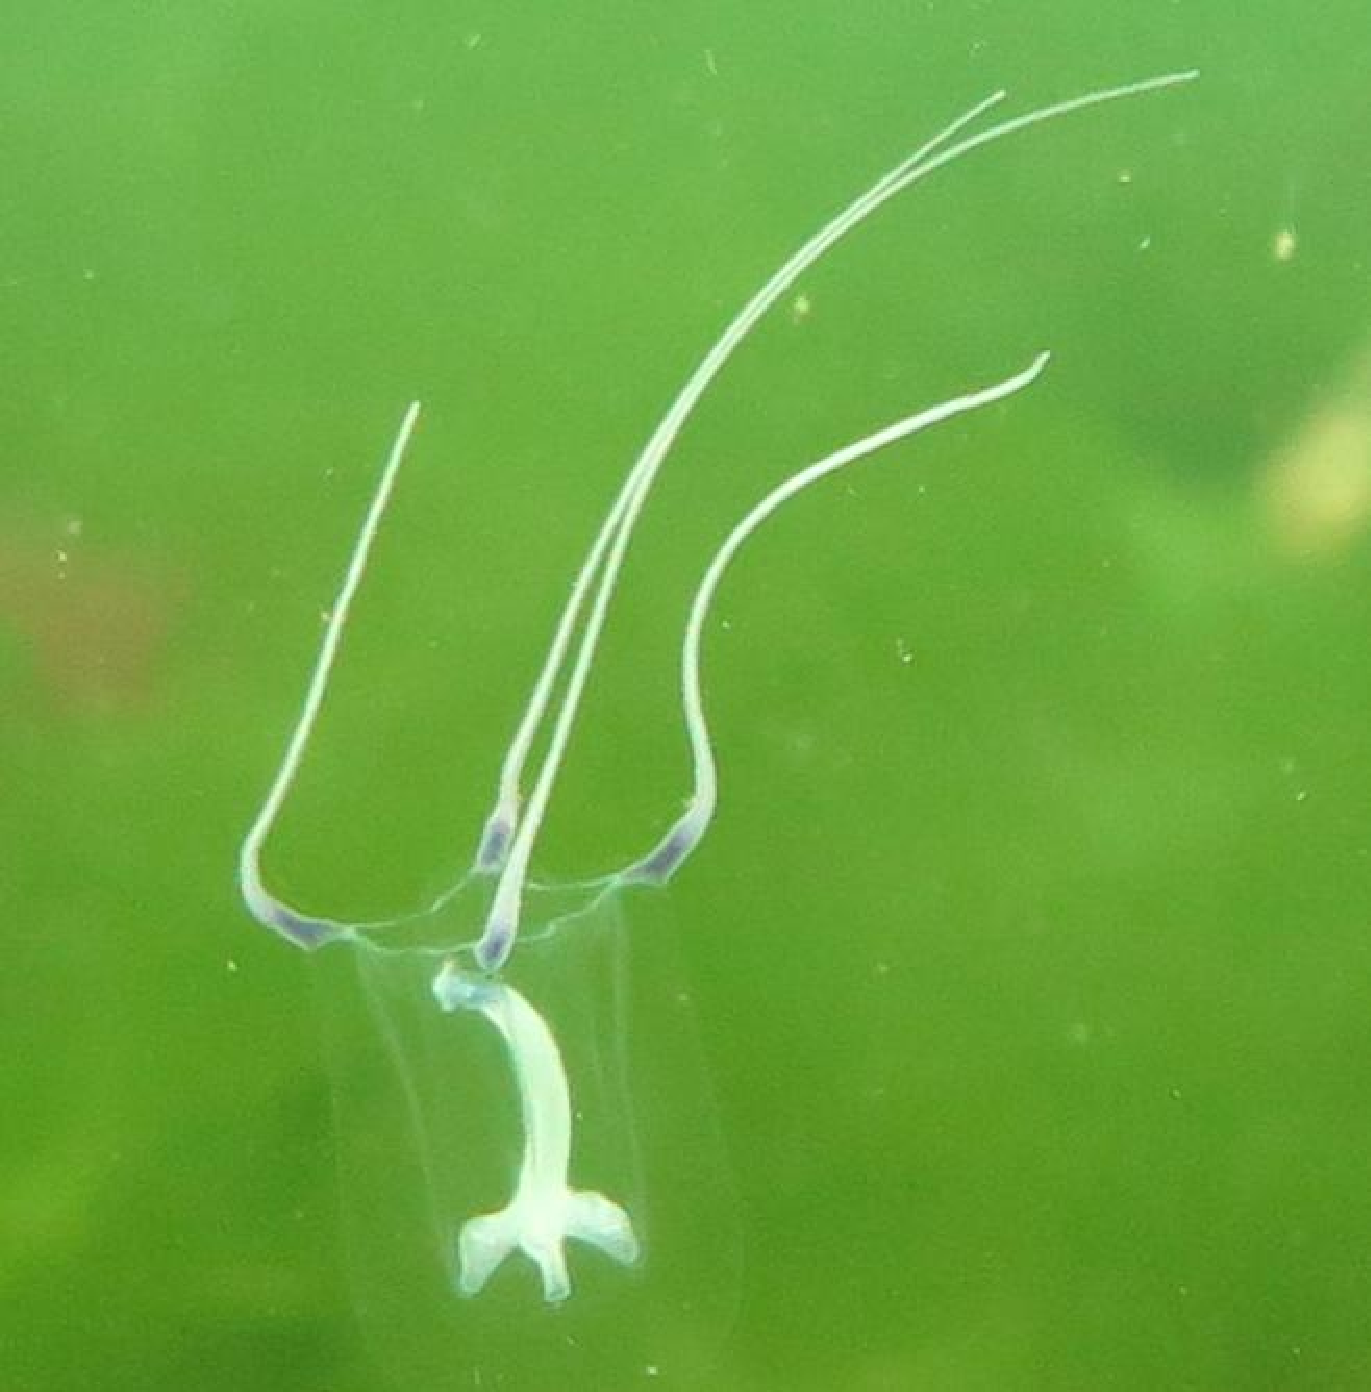
\includegraphics[height=9cm]{imgs/1901xx.pdf}
  \caption{Imagen original}
\end{minipage}
\hfill
\begin{minipage}[c]{0.48\linewidth}
  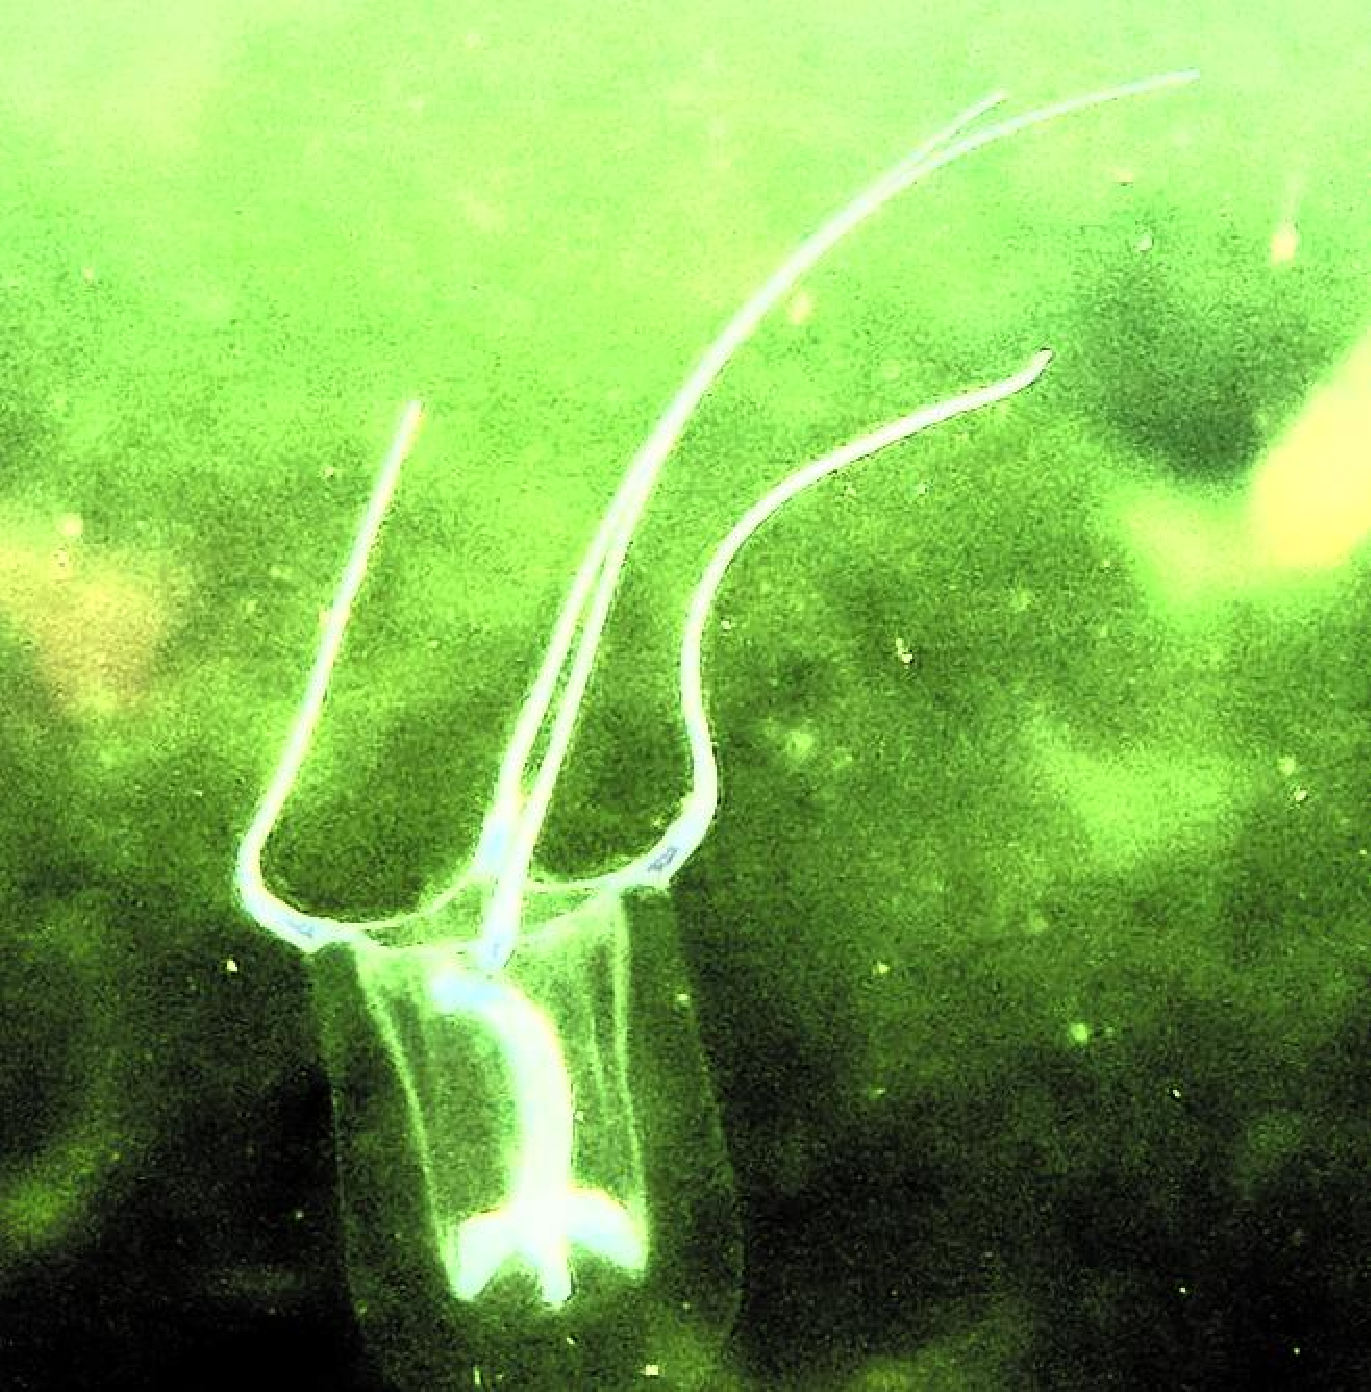
\includegraphics[height=9cm]{imgs/1901xxOut.pdf}
    \caption{$\alpha = 0.1, \beta = 0.8, \gamma = 0.1, [4, 1, 1]$}
\end{minipage}%
\end{figure}

\begin{figure}[H]
\begin{minipage}[c]{0.48\linewidth}
  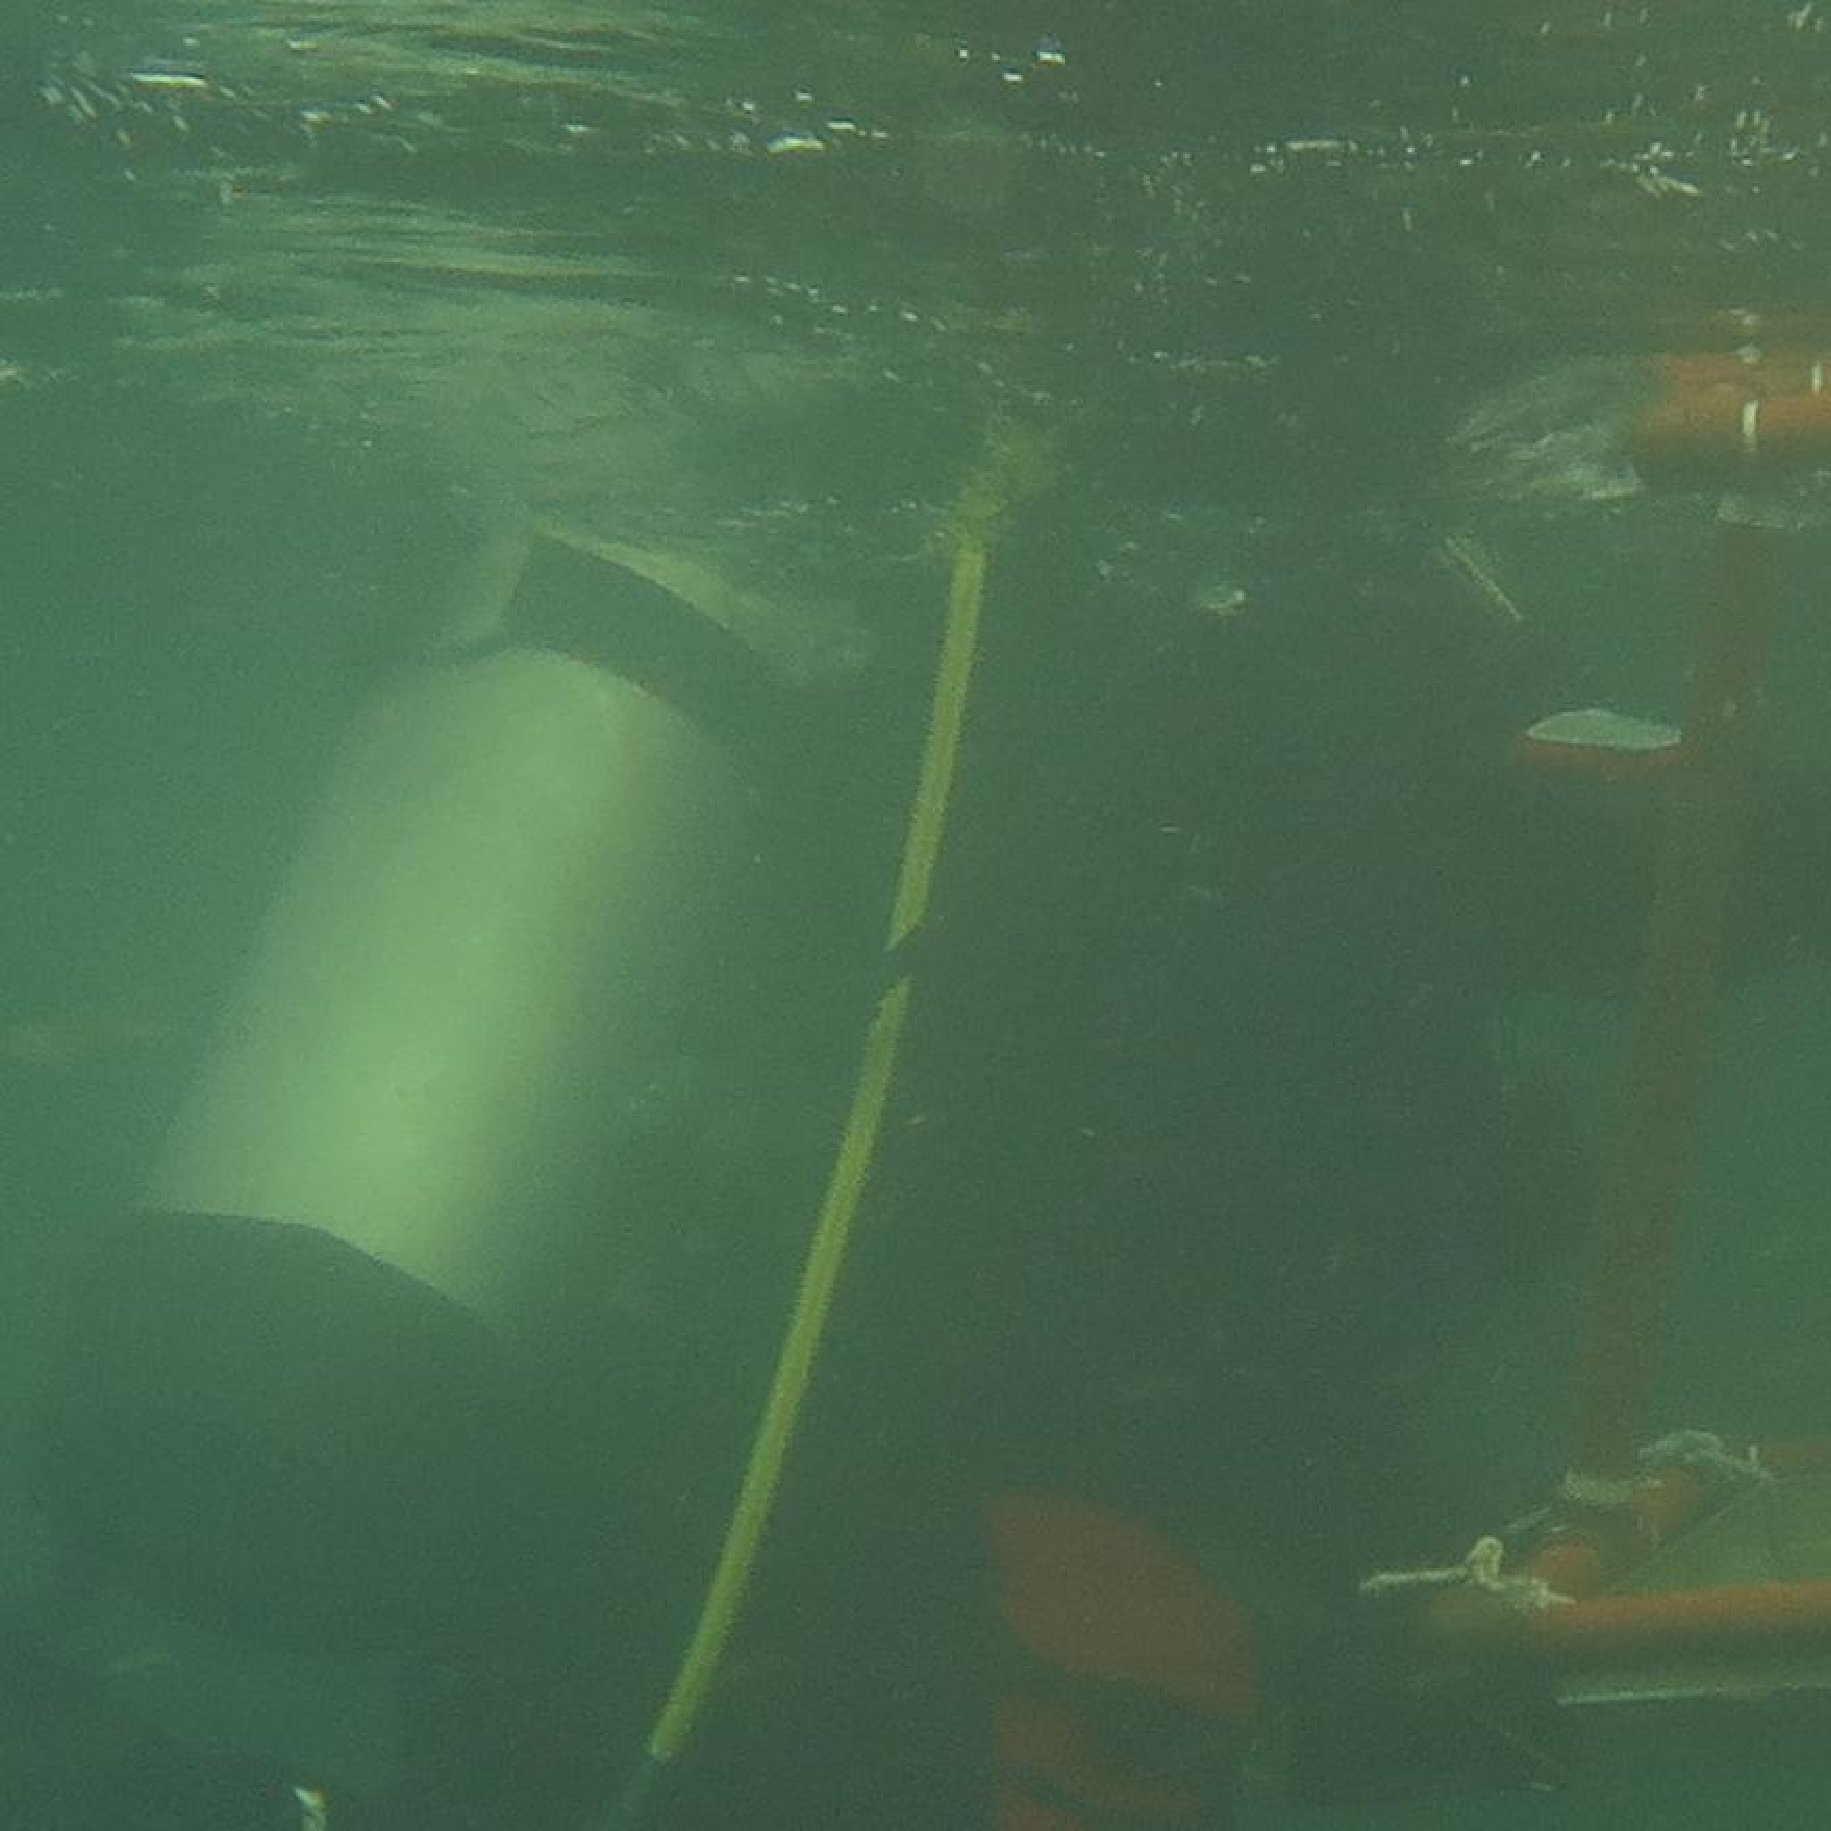
\includegraphics[height=9cm]{imgs/1908xx.pdf}
  \caption{Imagen original}
\end{minipage}
\hfill
\begin{minipage}[c]{0.48\linewidth}
  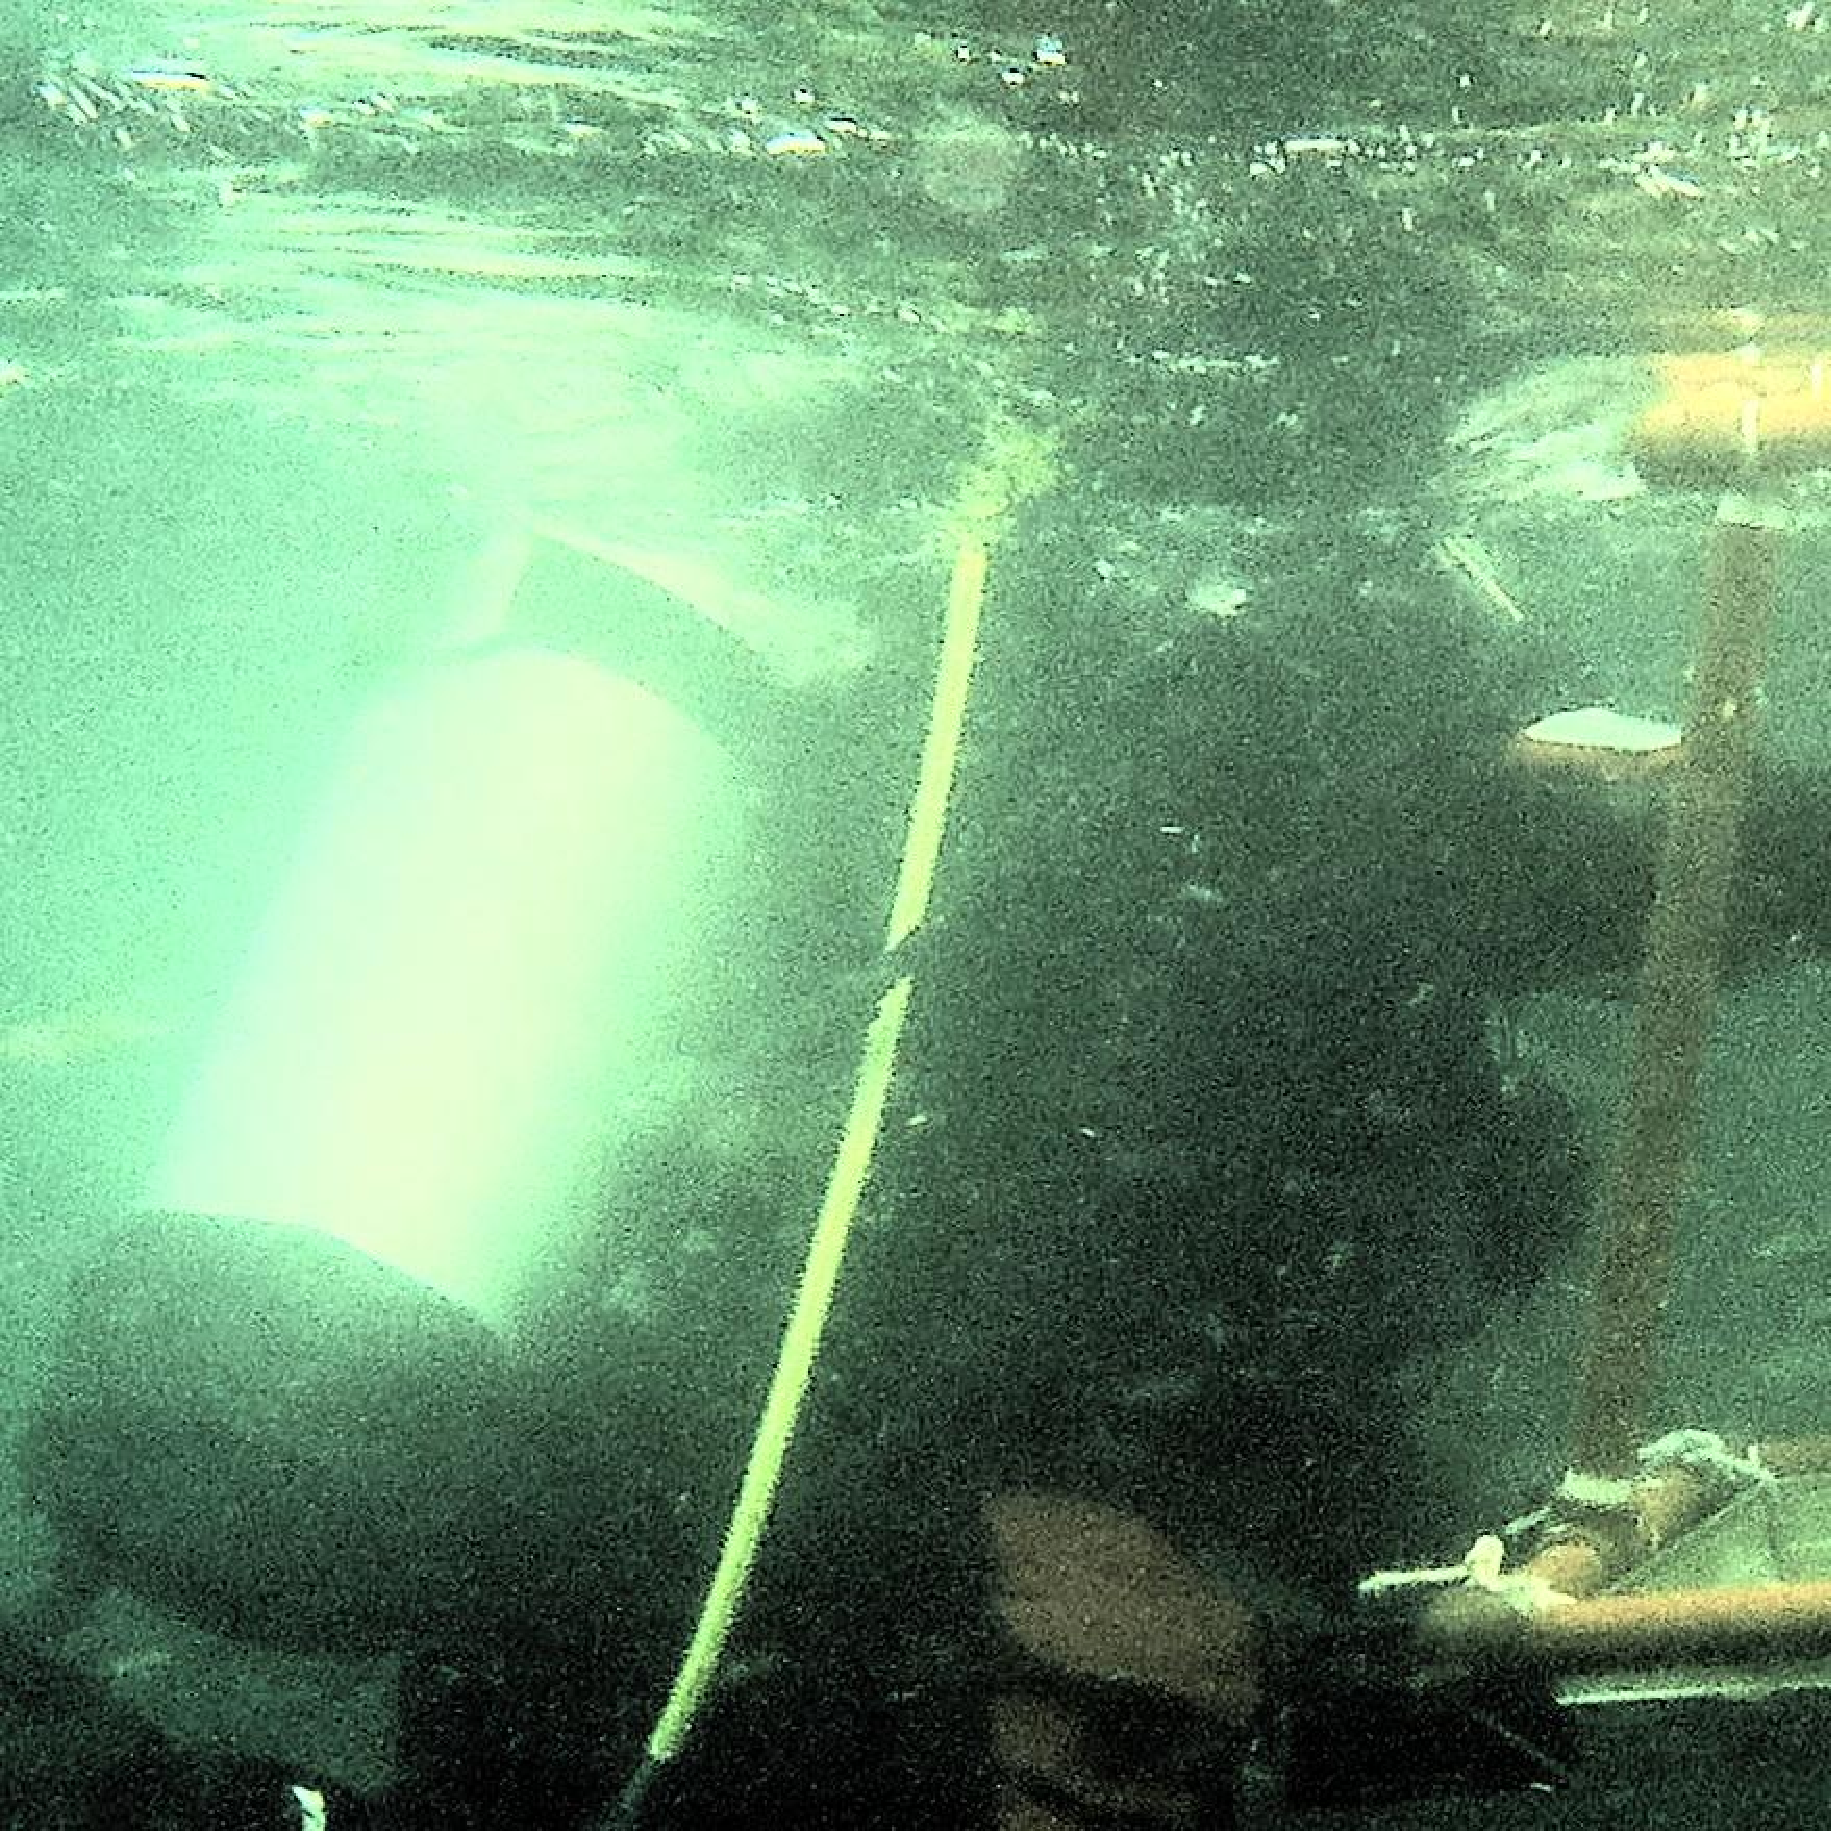
\includegraphics[height=9cm]{imgs/1908xxOut.pdf}
    \caption{$\alpha = 0.6, \beta = 0.1, \gamma = 0.3, [1, 4, 1]$}
\end{minipage}%
\end{figure}

\begin{figure}[H]
\begin{minipage}[c]{0.48\linewidth}
  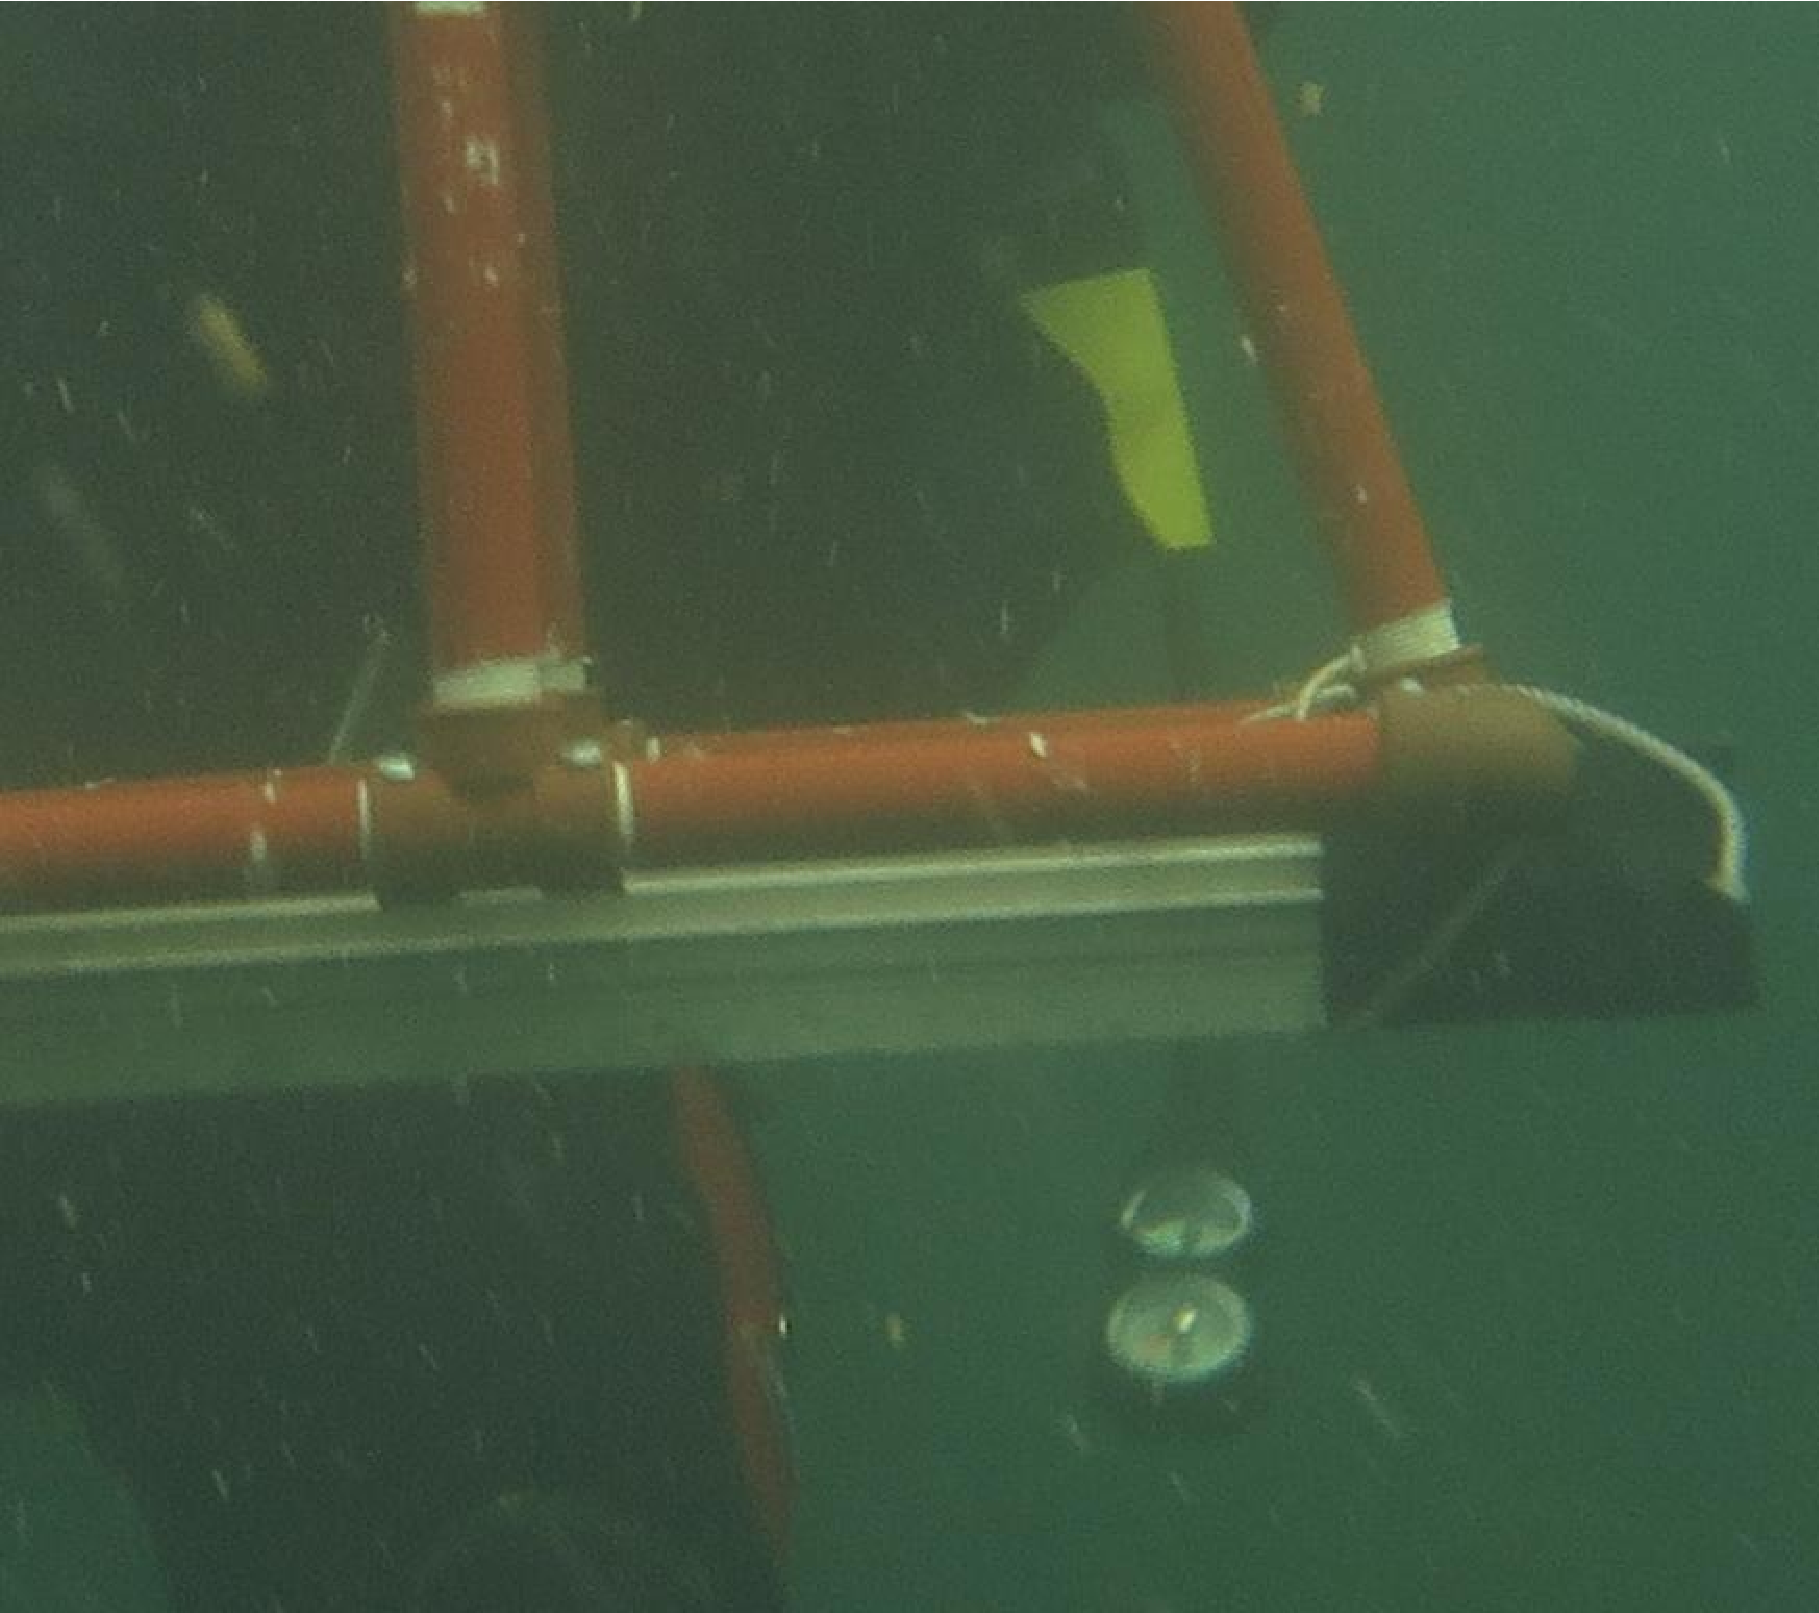
\includegraphics[height=8cm]{imgs/1907xx.pdf}
  \caption{Imagen original}
\end{minipage}
\hfill
\begin{minipage}[c]{0.48\linewidth}
  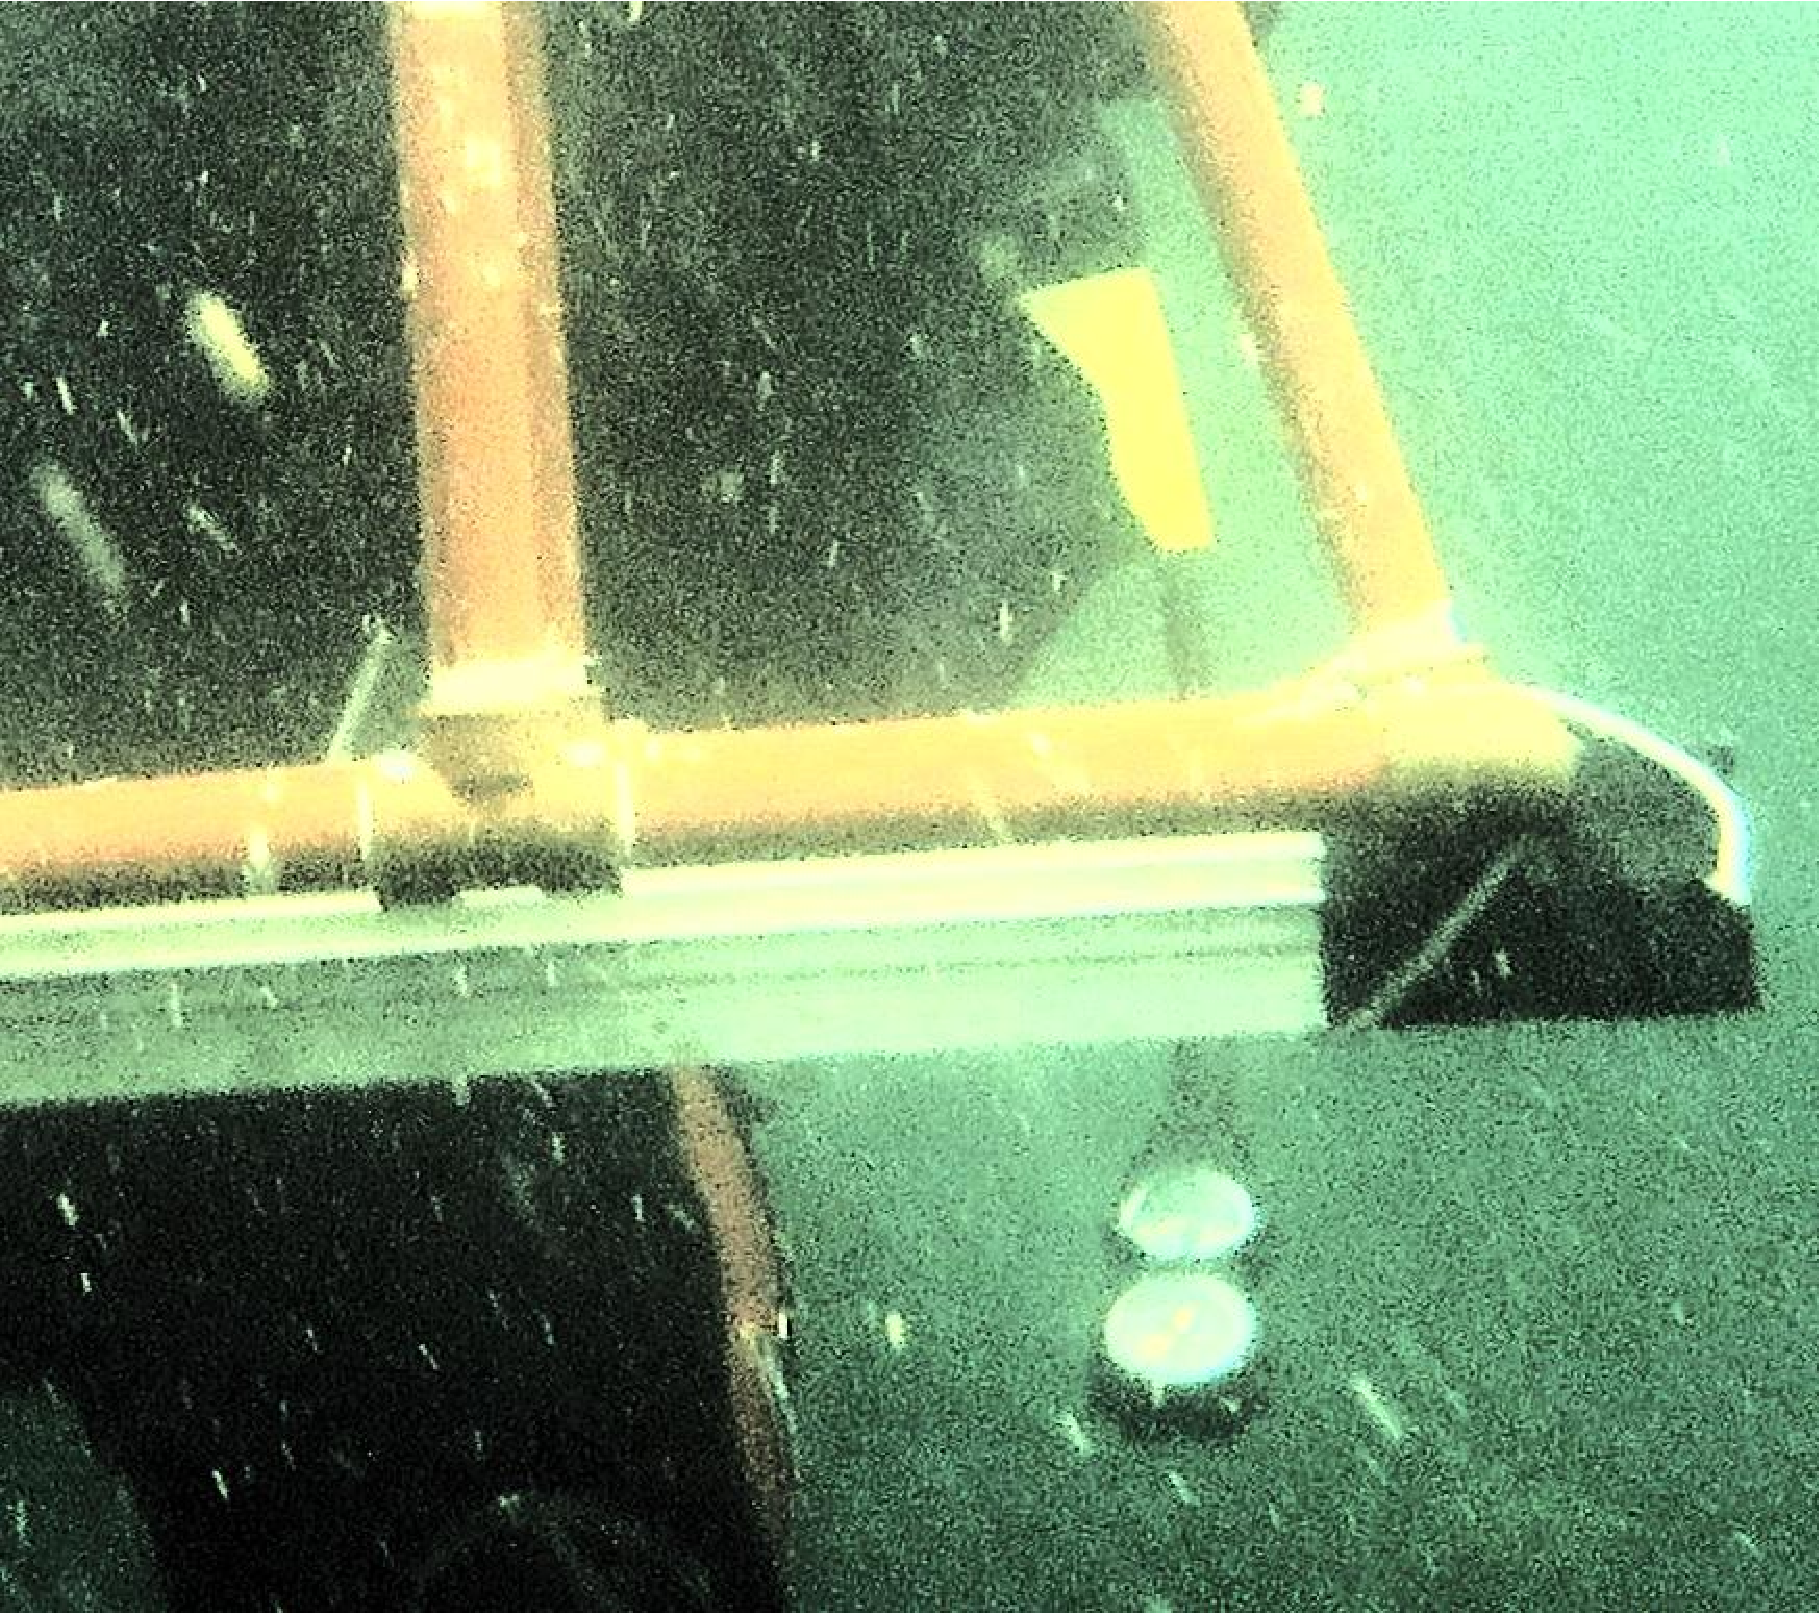
\includegraphics[height=8cm]{imgs/1907xxOut.pdf}
    \caption{$\alpha = 0.4, \beta = 0.4, \gamma = 0.2, [1]^{10}$}
\end{minipage}%
\end{figure}


\end{document}

